\documentclass[12pt,twoside]{article}
\usepackage{silence}
\WarningsOff*
\renewcommand{\abstractname}{\vspace{-\baselineskip}}
\usepackage[dvipsnames]{xcolor}
\usepackage[
linkcolor=darkgray,
colorlinks=true,
urlcolor=darkgray,
pdfstartview={XYZ null null 1.00},
pdfpagemode=UseNone,
citecolor={darkgray},
pdftitle={Holier Than Thou? No Large Partisan Gaps in the Consumption of Pornography Online}
]{hyperref}
\urlstyle{same}
\usepackage{geometry}
 \geometry{left=1.25in,top=1.7in}
\setlength{\parindent}{.5in}
\renewcommand{\baselinestretch}{1.3}
\setlength{\parskip}{\baselineskip}
\usepackage{xcolor}
\usepackage{fancyhdr}
\renewcommand{\headrulewidth}{0pt}
\usepackage[labelfont=bf]{caption}
\captionsetup[figure]{labelfont={bf},name={Figure},labelsep=period}
\usepackage{natbib}
\bibliographystyle{apalike}
\usepackage{graphicx}
\graphicspath{{../}}
\usepackage{float}
\usepackage{booktabs}
\usepackage{tabularx}
\usepackage{titling}
\usepackage{amsmath}
\usepackage{placeins}
\usepackage{subcaption}
\usepackage{lscape}
\usepackage{pdflscape}
\usepackage{adjustbox}
\usepackage{dcolumn}
\usepackage{moresize}
\usepackage[nameinlink, capitalize, noabbrev]{cleveref}
\settowidth{\thanksmarkwidth}{*}
\setlength{\thanksmargin}{-\thanksmarkwidth}
\usepackage{titlesec}
\setlength{\droptitle}{-5em}
\setlength\thanksmarkwidth{.5em}
\setlength\thanksmargin{-\thanksmarkwidth}
\titleformat{\section}{\normalfont\bfseries\filcenter}{}{0pt}{}
\titleformat{\subsection}{\normalfont\bfseries\filcenter}{}{0pt}{\itshape}
\titleformat{\subsubsection}{\normalfont\bfseries\filcenter}{}{0pt}{\itshape}
\titlespacing*{\section}
  {0pt}{-.1\baselineskip}{-.1\baselineskip}  
\titlespacing*{\subsection}
   {0pt}{-.1\baselineskip}{-.1\baselineskip}  

\usepackage[T1]{fontenc}
\usepackage{fontspec}
\fontspec{Times New Roman}
\date{}
\providecommand{\keywords}[1]
{
   \small	
  \textit{\hspace{-1em} Keywords: } #1
}
\newfontfamily\headingfont[]{Arial}
%Add Author names to headers and footers here:
\fancypagestyle{firstpage}{
  \fancyhf{}% clear all fields
  \fancyfoot[L]{\color{gray} \footnotesize Copyright \copyright 2024 Lucas Shen and Gaurav Sood. Licensed under the Creative Commons Attribution Non-commercial No Derivatives (by-nc-nd). Available at: \url{http://journalqd.org}}%
  \lhead{\color{gray} \footnotesize Journal of Quantitative Description: Digital Media 1(2021), 1–n}
\rhead{\color{gray} \footnotesize 10.51685/jqd.2024.011}
}
\pagestyle{fancy}
\fancyhf{}
\fancyhead[LO]{\color{gray} \footnotesize Journal of Quantitative Description: Digital Media 1(2024)}
\fancyhead[RO]{\color{gray} \footnotesize Consumption of Pornography Online \thepage}
\fancyhead[LE]{\color{gray} \footnotesize Lucas Shen and Gaurav Sood}
\fancyhead[RE]{ \color{gray} \footnotesize Journal of Quantitative Description: Digital Media 1(2024) \thepage}
% DO NOT MAKE CHANGES ABOVE THIS LINE
%Article Title goes here
\title{\normalsize \headingfont \textbf{Holier Than Thou? No Large Partisan Gaps in the Consumption of Pornography Online} \vspace{-1.5em}} 
%Author names and affiliations go here, any Acknowledgements / authors' note / disclosure statement goes into \thanks{}
\author{\normalsize Lucas Shen\\ \normalsize National University of Singapore, Singapore
\vspace{1em} \\ \normalsize Gaurav Sood \\ \normalsize Independent Researcher, USA \thanks{Lucas Shen: \href{mailto:lucas@lucasshen.com}{lucas@lucasshen.com}}\thanks{Gaurav Sood: \href{mailto:gsood07@gmail.com}{gsood07@gmail.com}}\thanks{Date submitted: 2023-03-13}} 
\usepackage{lipsum}
\renewcommand\footnotemark{}
\begin{document}
\maketitle
\thispagestyle{firstpage}
\vspace{-8em}

\begin{abstract}
  Consumption of pornography has been blamed for a variety of societal ills, including the rise in misogyny, sex crimes, and the coarsening of the culture. Using passively collected browsing data from YouGov, we investigate how much pornography Americans consume online. We find that there is a sharp positive skew in the consumption of pornography, with a small number of users consuming lots of pornography and most consuming small amounts. Only about 32 percent of respondents consumed pornography online during the month-long observation period. Of the people who consumed pornography, the median consumer spent about three-quarters of an hour consuming pornography, and 95 percent of the consumers spent less than five and a half hours. Lastly, we find, in line with previous research \citep{macinnis2015american, edelman2009markets}, which was based on aggregated data, that Republicans consume somewhat more pornography online than Democrats. Adjusting for immutable characteristics like age and gender makes the differences go away.
\emph{Keywords:} Measurement, YouGov, Pornography, Partisanship, Quantile Regression, Online Consumption
\end{abstract}

\keywords{\textit{measurement, YouGov, pornography, partisanship, quantile regression, online consumption} \vspace{8ex}}

\section{Introduction}\label{sec:intro}
Pornography consumption has been rising steadily  \citep{Perry2018-cw, Price2016-sm, Wright2013-gl}. Consumption of pornography is associated with a variety of disturbing attitudes, beliefs, emotions, and behaviors. Consuming pornography is associated with support for violence against women \citep{hald2010pornography, malamuth2012pornography, donnerstein1984pornography}, belief in rape myths \citep{foubert2011pornography}, increased gender role conflict, lesser sexual satisfaction \citep{szymanski2014psychological, stewart2012young}, poorer relationship quality \citep{szymanski2014psychological, szymanski2015male}, and sexually risky behaviors such as engaging in paid sex and having extramarital sex \citep{wright2012internet}. A lot of popular pornography also contains a healthy dose of violence \citep{Vera-Gray2021-qv}. An analysis of popular pornography revealed that 88.2\% of the scenes contained physical aggression and 48.7\% verbal aggression \citep{bridges2010aggression}. The increased accessibility of online pornography also raises concerns about adolescent sexual development \citep{Peter2016-de, Ybarra2005-id}. For all these reasons, there are serious concerns about the consumption of pornography.\footnote{This is despite the fact that the studies cited above do not provide rigorous evidence for the negative impact of pornography consumption \citep{Ferguson2022-fo, Pathmendra2023-fx, Peter2016-de}.}

In this paper, we investigate how much pornography Americans consume online. Using passive tracking data on online browsing from YouGov, we find a sharp skew in the consumption of pornography, with a small set of users consuming a large chunk of pornography. About 68 percent of respondents abstained from consuming pornography online during the month-long observation period. Of the people who consumed pornography, the median consumer spent about 45 minutes consuming pornography, and the 95th percentile consumer spent close to 20 hours. % (Table SI 1.2)

We also use the data to contribute to the small literature connecting political conservatism to opposition to pornography \citep{Peek1982-ua, Woodrum1992-vk}. Despite the expected relationships between religiosity, political conservatism, and opposition to pornography \citep{Wright2013-an, Perry2018-cn}, recent research, using aggregate data has shown that politically conservative states search for pornography more often and subscribe to online adult services more often \citep{macinnis2015american, edelman2009markets}. Combining individual-level data on partisanship with directly measured pornography consumption, we shed light on whether Democrats consume more pornography than Republicans or vice versa. Superficially, our browsing data suggest Republicans in the right tail of the distribution consume more online pornography than Democrats. Adjusting for background attributes like age, gender, etc., however, makes the partisan differences go away. Our findings relate to \cite{Perry2018-cn}, who find that higher levels of religiosity, also linked to political conservatism, are associated with views of pornography as morally wrong while still having viewed pornography. This unexpected finding suggests a discordance between survey responses and reported actions. Republicans may be consuming just as much pornography as Democrats; they are simply saying otherwise. 


\section{Data and Methods}
\label{sec:data}

\subsection{Online Browsing Data}
\label{subsec:online_browse_data}

We use data from YouGov to measure the consumption of adult content online. YouGov maintains a large panel that it recruits through various methods. It uses matched sampling to survey respondents: it draws a random sample from a large synthetic representative sampling frame, finds respondents that match the sampled individuals from its panel, and invites them to take a survey. (For data on how well YouGov surveys approximate results from the census and other high-quality government surveys, see \citet{rivers2009, graham2021advantages, foote2021measuring}.) YouGov also collects de-identified web browsing data via passive metering software, RealityMine, which some panelists volunteer to have installed in lieu of rewards. RealityMine captures online visits independent of browser type or browser-specific privacy settings.

Specifically, we use data from 1,200 YouGov panelists for June 2022 \citep{data-dataverse}. These 1,200 panelists visited the web nearly 6 million times. For each visit, we have the anonymized URL, domain (e.g., wikipedia.org), the time of the visit, the length of the visit, and the type of content. 

\subsection{Demographics And Partisan Identification}
\label{subsec:demographics}
YouGov panel file contains data on demographic characteristics like birth year, state of residence, gender, race, and education level. It also contains data on partisan self-identification. Except for 120 respondents who did not respond or picked ``not sure'' or ``don't know,'' the rest selected the party they identified with or marked themselves as independents. Of the 1,080 people, 82\% leaned either Republican or Democrat. The remaining 18 percent identified as independent. (See Panel B of \cref{tab:characteristics_split_by_party} for a summary of socio-demographic data by party.)

\subsection{Measuring Pornographic Content}
\label{subsec:measuring_porn_content}

Our main analysis uses classifications provided by YouGov. Of the 6 million visits to 855,564 unique anonymized URLs, YouGov provides data on the kind of content hosted (e.g., Shopping, Business, Adult) for 727,681 unique URLs (making up 85\% of all visits). To illustrate the granularity of the categorization, \url{https://www.google.com/search?ANONYMIZED} is categorized as ``Search Engines and Portals'' while \url{https://mail.google.com/mail/u/0/} is categorized as ``Chat and Instant Messaging.'' 

To code pornographic content, we start by assuming all content marked ``Adult'' as pornographic. This includes ``Adult, Business'' (e.g., onlyfans.com) and ``Adult, Entertainment'' (e.g., hentainfox.com). YouGov classifies some domains that do not primarily carry pornographic content, e.g., urbandictionary.com and 4chan.org, as Adult. Given the skew in the data (see \cref{fig:top25_adult} and \cref{fig:top25_nonadult}), we manually checked the top few hundred adult domains (constituting well over 99\% of the adult content consumed) to remove such sites. We code a domain as carrying pornographic content if there is nudity on the landing page or if the site is some form of erotica. Domains without a YouGov category are assumed to be missing completely at random. 

In \hyperref[sm:smE]{Appendix E}, we leverage \texttt{piedomains} and a Google service, Virustotal, to assess whether our results are robust to alternate ways of measuring the kind of content accessed by people. \texttt{piedomains} uses open-source domain classification lists to train a neural network that learns the relationship between the kind of content hosted by a domain and the text on the homepage and homepage screenshots of websites \citep{Chintalapati_piedomains_Predict_the_2022}. 
VirusTotal collates domain classification data from different private services. Based on their data coverage of our domain data, we use the top three services: Forcepoint ThreatSeeker, Bitdefender, and alphaMountain.\footnote{Forcepoint ThreatSeeker, Bitdefender, and alphaMountain, respectively, cover 47,950, 43,391, and 36,063 of the roughly 64,000 unique domains the panelists visited over the month.}


\section{Results}\label{sec:results}
\subsection{Most Visits Are to a Few Websites}
\label{subsec:concentration_media_consumption}

In line with previous research \citep{hindman2009myth, Dewan2004-tt}, we find a considerable skew in online media consumption (see \cref{fig:top25_nonadult} and \cref{fig:top25_adult} in \hyperref[sm:smA]{Appendix A}). As \cref{fig:top25_nonadult} shows, the big tech and social media companies occupy most of the top 25 most frequently visited websites. The top 5 non-pornographic sites were visited more than 200,000 times by our panelists. In comparison, the 99th percentile non-pornographic site was visited only 1,652 times by our panelists during the observation period. 

There is a similar concentration of visits in adult content, with a few adult sites attracting a bulk of the total traffic. \cref{fig:top25_adult} reports the top 25 pornography sites. The top three pornography sites (``\textit{xvideos.com}'', ``\textit{pornhub.com}'', and ``\textit{xnxx.com}'') are visited more than 6,500 times by the people in our sample during the one-month period. The most visited site, xvideos.com, clocked 311 hours in total from our participants who visited a pornographic site. (Given 361 consumers of online pornography, this translates into an average of 52 minutes of consumption of \textit{xvideos.com} per participant.) Newer platforms such as ``\textit{onlyfans.com}'' are among the most visited pornography sites. Nine sites are above the 99th percentile in pornography visits (2,224 visits). The average time spent on the ten most frequented pornography sites is 12x the average time on all other pornography sites (approximately 109 minutes vs. 9 minutes, \cref{fig:concentration_porn_consumption}). Our finding is consistent with other analyses of traffic to pornographic sites \cite{webporn}.
The average time spent on the ten most frequented pornography sites is 12 times the average time spent on all other pornographic sites (approximately 109 minutes vs. 9 minutes, \cref{fig:concentration_porn_consumption}). This finding is consistent with other analyses of traffic to pornographic sites \citep{webporn}.

In all, in line with other studies on online media consumption \citep{Dewan2004-tt, hindman2009myth, webporn}, we find that a few sites attract most of the traffic online.

\subsection{Consumption of Pornography Online}
\label{subsec:concentration_in_porn}

\begin{figure}[!ht]
\caption{Hours Spent on Online Pornography and All Other Online Content}
\label{fig:distribution_duration_on_adultsites_fullsample}
     \centering
     \begin{subfigure}[b]{0.495\textwidth}
         \centering
         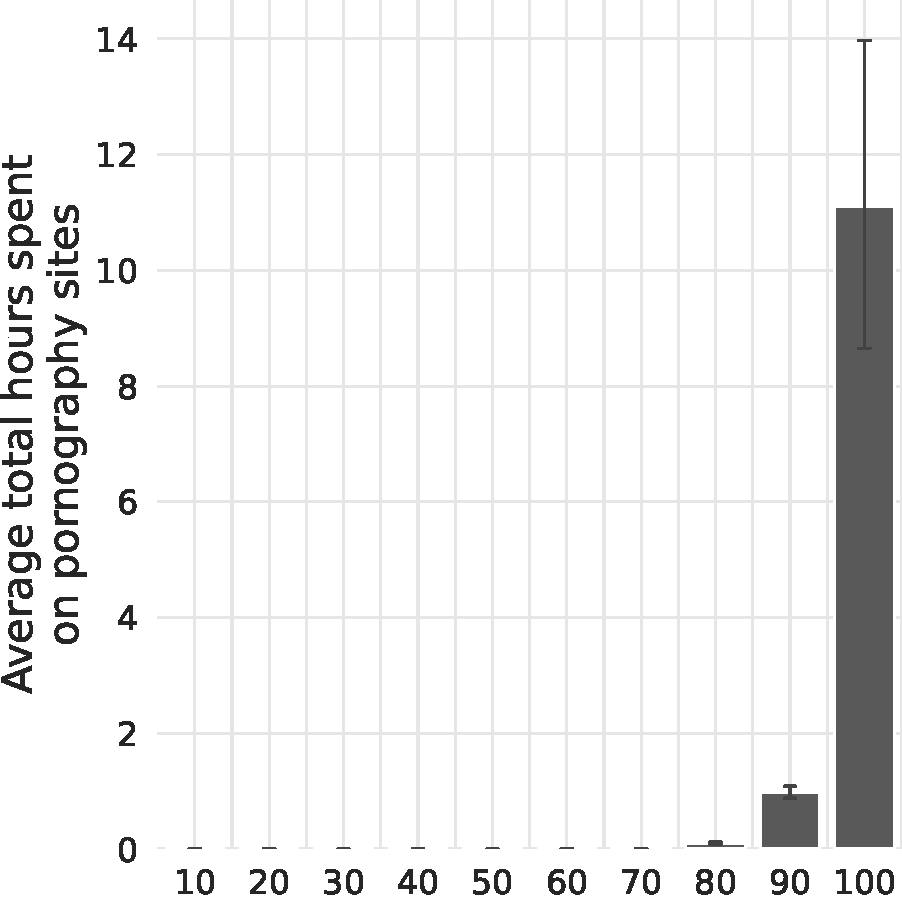
\includegraphics[width=\textwidth]{figs/distribution_duration_on_adultsites_fullsample.pdf}
         \caption{Online pornography}
     \end{subfigure}
     \hfill
     \begin{subfigure}[b]{0.495\textwidth}
         \centering
         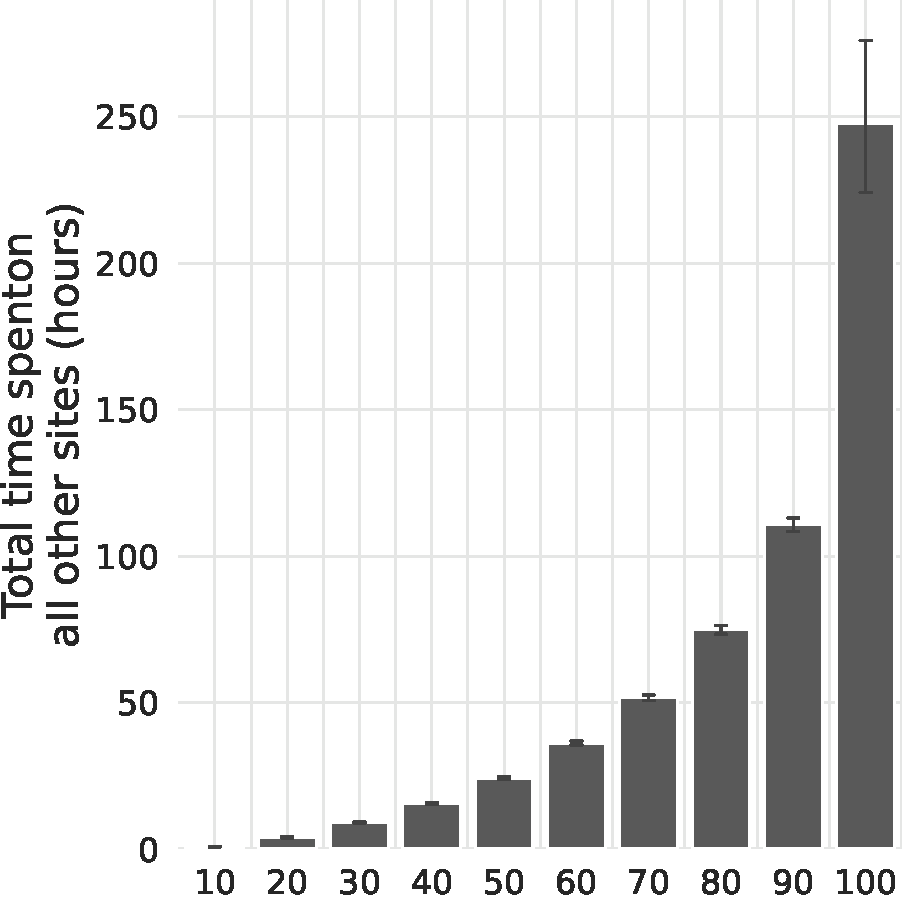
\includegraphics[width=\textwidth]{figs/distribution_duration_on_nonadultsites_fullsample.pdf}
         \caption{Other online content}
     \end{subfigure}
\caption*{\footnotesize \emph{Notes:} 
    Each panel shows the total number of hours for the sample period.
    Individuals (n = 1135) are split into deciles, with each bin containing approximately the same number of individuals.
    The height of the bars indicates the mean of each bin. 
    Capped vertical bars are bootstrapped 95\% confidence intervals (n = 10,000).
    %textbf{FIG??} shows the same figures but only for consumers of pornography.
}
\end{figure}

\cref{fig:distribution_duration_on_adultsites_fullsample} plots hours spent on pornography sites and all other online content for the entire sample. Consumption of online pornography pales in comparison to all other online content. Only 31.8 percent of the respondents consumed any pornography online during the observation period (see column 3 of \cref{tab:characteristics_split_by_party}). Of the 31.8 percent of the respondents who consumed any pornography during the month, the median consumer consumed less than an hour of pornography (approximately 42 minutes), while the 80th percentile consumer consumed nearly 4.5 hours and the 95th percentile almost 20 hours or about 40 minutes per day (see \cref{tab:distribution_duration}). A similar picture arises when it comes to the proportion of time spent online consuming pornography--the 50th percentile consumer spent about 3.1 percent of their time on online pornography. For the 80th percentile, this is about 14 percent, and for the 95th percentile, this is about 58.5 percent (see \cref{tab:distribution_prop_duration}).

To help contextualize the above figures, we present statistics on time spent consuming content from the top ten non-adult categories in \cref{tab:top10cat_description}. The median pornography consumer spends more hours on adult content than sites from six non-adult categories. Only three categories, ``Chat and Instant Messaging'' (e.g., google.com, yahoo.com, live.com), ``Business, Social Networking'' (e.g., facebook.com, soocial.com)),  and ``Entertainment, Streaming Media'' (e.g., youtube.com, hulu.com, netflix.com), have higher levels of consumption at the 95th percentile than online pornography.

\subsection{Substitution?}
Are people substituting pornography for other kinds of leisure content? To shed light on that, we examine the relationship between the time spent on online pornography vs. time spent on other leisure-related online sites. We fit locally weighted linear regression after removing extreme values (90th percentile) in online consumption. At the left tail of online pornography (below 0.5 hours), increases in pornography consumption are associated with fewer hours spent on non-adult-related shopping sites (\cref{fig:tu_prop_entertainment-prop_adult_duration}). Otherwise, there are no salient patterns of substitution in time spent on online pornography vs. other leisure sites.

\begin{figure}[!ht]
\caption{Time Spent on Online Pornography vs. Non-adult Leisure}
\label{fig:tu_prop_entertainment-prop_adult_duration}
     \centering
     \begin{subfigure}[b]{0.495\textwidth}
         \centering
         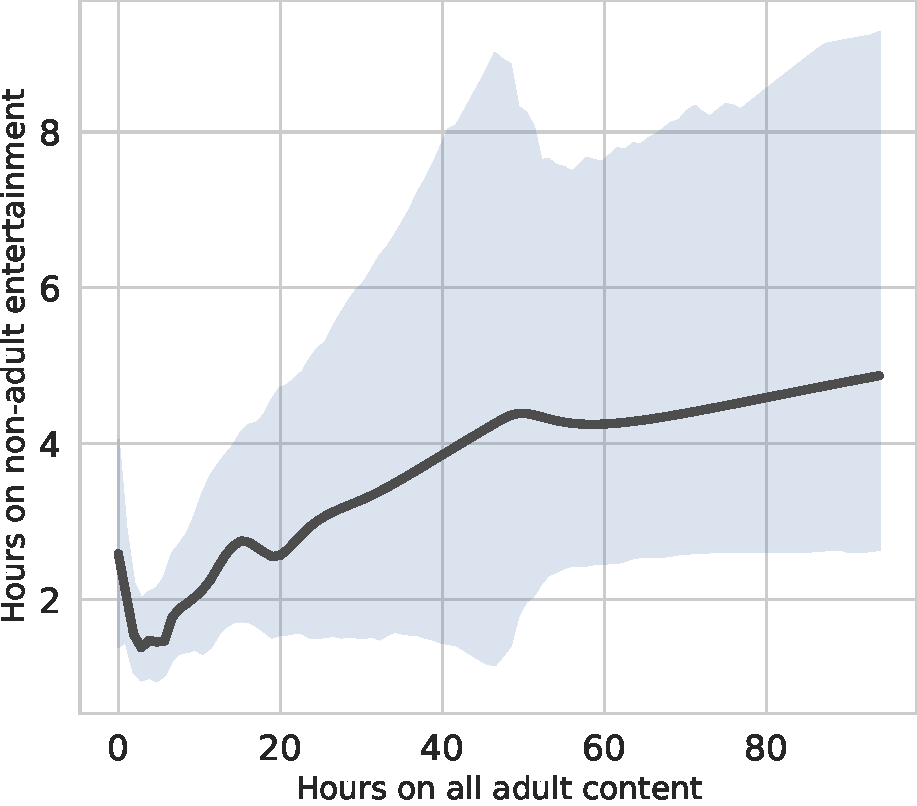
\includegraphics[width=\textwidth]{figs/tu_duration_entertainment-duration_adult.pdf}
         \caption{Entertainment}
     \end{subfigure}
     \hfill
     \begin{subfigure}[b]{0.495\textwidth}
         \centering
         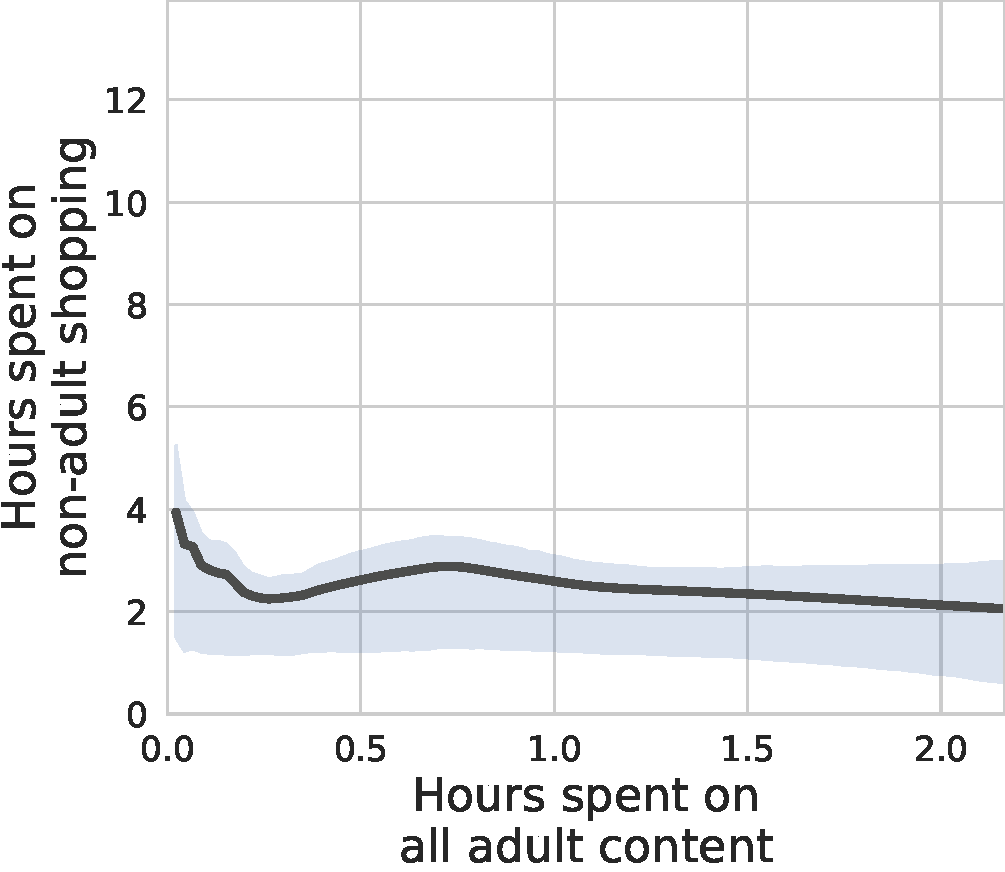
\includegraphics[width=\textwidth]{figs/tu_duration_shop-duration_adult.pdf}
         \caption{Shopping}
     \end{subfigure}
\caption*{\footnotesize \emph{Notes:} Lowess between time spent on online pornography and time spent on other non-adult leisure (``entertainment'' and ``shopping''). Observations above the 90th percentile for adult content consumption are omitted to prevent the graph from being dominated by these outliers. (Given we plot a lowess, such truncation doesn't change the relationship we show.) Non-adult entertainment sites are those with YouGov categories containing ``entertainment'' (e.g., ``Entertainment, Streaming Media'', ``Education, Entertainment, Streaming Media'', ``Business, Entertainment'', etc.)---top five such sites are youtube.com, hideout.co, hulu.com, netflix.com, and yahoo.com. Non-adult shopping sites are those with YouGov categories containing ``shopping'' (e.g., ``Shopping'', ``Business, Shopping'', ``Messageboards and Forums, Shopping'', etc.)---the top five such sites are amazon.com, ebay.com, walmart.com, etsy.com, capitaloneshopping.com, and craigslist.org. Each estimation in the Lowess uses .3 of the sample data.
The 95\% confidence intervals shaded in blue are bootstrapped (n = 1000). Swapping the horizontal axis for adult content excluding adult-related entertainment and shopping sites looks similar (see \cref{fig:tu_prop_entertainment-prop_pure_adult} in \hyperref[sm:smC]{Appendix C}). 
}
\end{figure}

\subsection{Partisan Differences}
\label{subsec:partisan_differences}
As \cref{tab:characteristics_split_by_party} shows, 31.5\% of Democrats consumed at least some pornography over the month vs. 29.4\% of Republicans. The 2\% difference is not statistically significant. Of the partisans who consumed any pornographic content online, \cref{tab:distribution_duration_party} presents the distribution of time spent on pornographic sites by partisan leanings. Republicans spent more time consuming online pornography than Democrats. The median Republican consumer of pornography consumed 1.4 hours of pornography, while the median Democratic consumer of pornography consumed 0.5 hours. A two-sample Kolmogorov-Smirnov test for differences in distribution rejects the null hypothesis (p = .005) (\cref{tab:distribution_duration_party}). In \cref{tab:distribution_prop_duration_party}, we observe similar patterns for time spent on pornography sites as for percentage of total time spent on the web. The median Republican consumer of pornography consumes 4 percent of their online time on pornography, while the median Democratic consumer of pornography consumes 1.3 percent.

%===========================
% Quantile regressions
% Hours spent on adult sites
%===========================
\begin{figure}[t]
	\centering
	\caption{Distribution of Partisan Differences in Hours Spent on Pornographic Sites}
	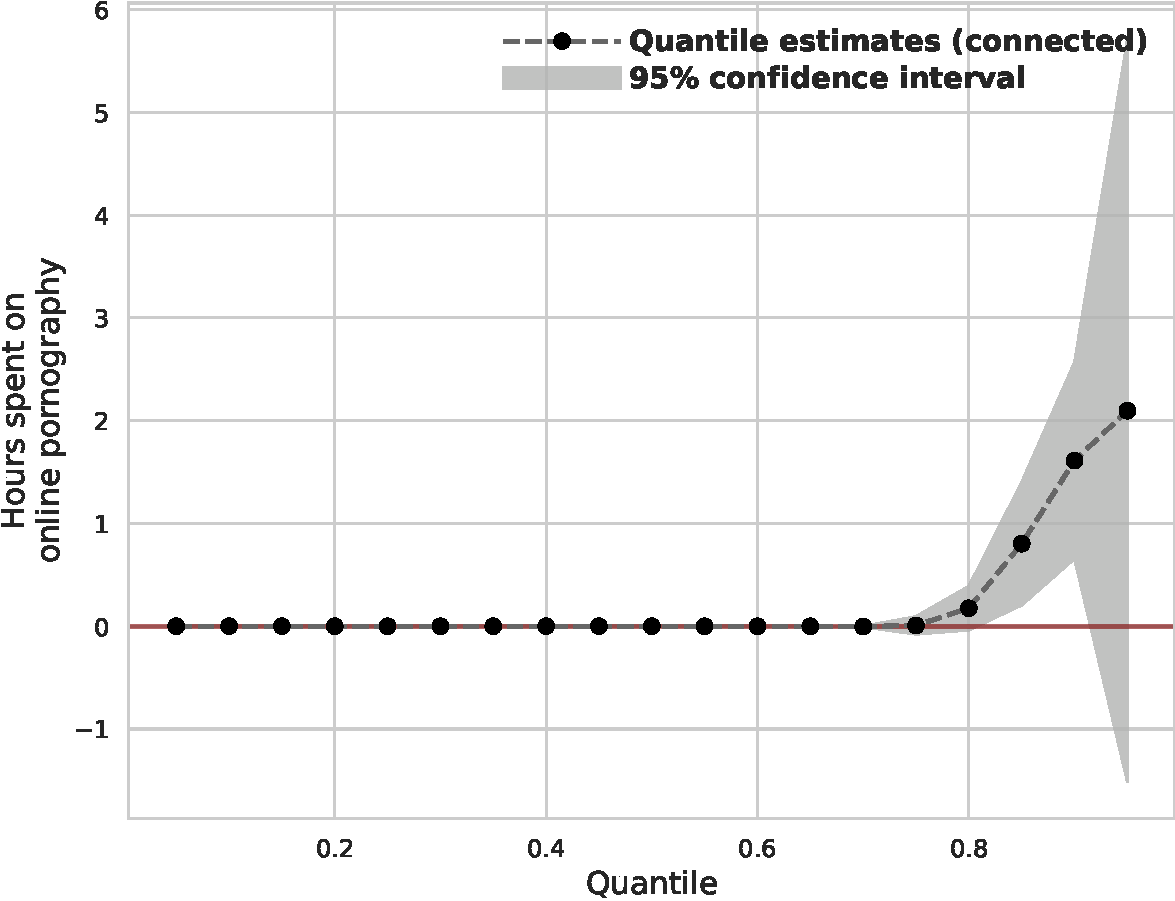
\includegraphics[width=.7\linewidth]{figs/quantile_reg_duration_adult.pdf}
	\caption*{\footnotesize \emph{Notes:} 
		The dependent variable is the number of hours individuals in our sample spent on pornographic sites.
		Each point indicates the difference between Republicans and Democrats and corresponds to a quantile regression at the quantile indicated by the x-axis.
		95\% confidence intervals constructed from standard errors.
		See \cref{fig:quantile_regression_duration_covariates} for the same plot controlling for individual characteristics.
        \cref{tab:quantile-estimates-hours} in \hyperref[sm:smB]{Appendix B} tabulates the estimates.
	}
	\label{fig:quantile_regression_duration}
\end{figure}

%========================================
% Quantile regressions
% Proportion of time spent on adult sites
%========================================
\begin{figure}[t]
	\centering
	\caption{Distribution of Partisan Differences in the Percentage of Time Spent on Pornographic Sites}
	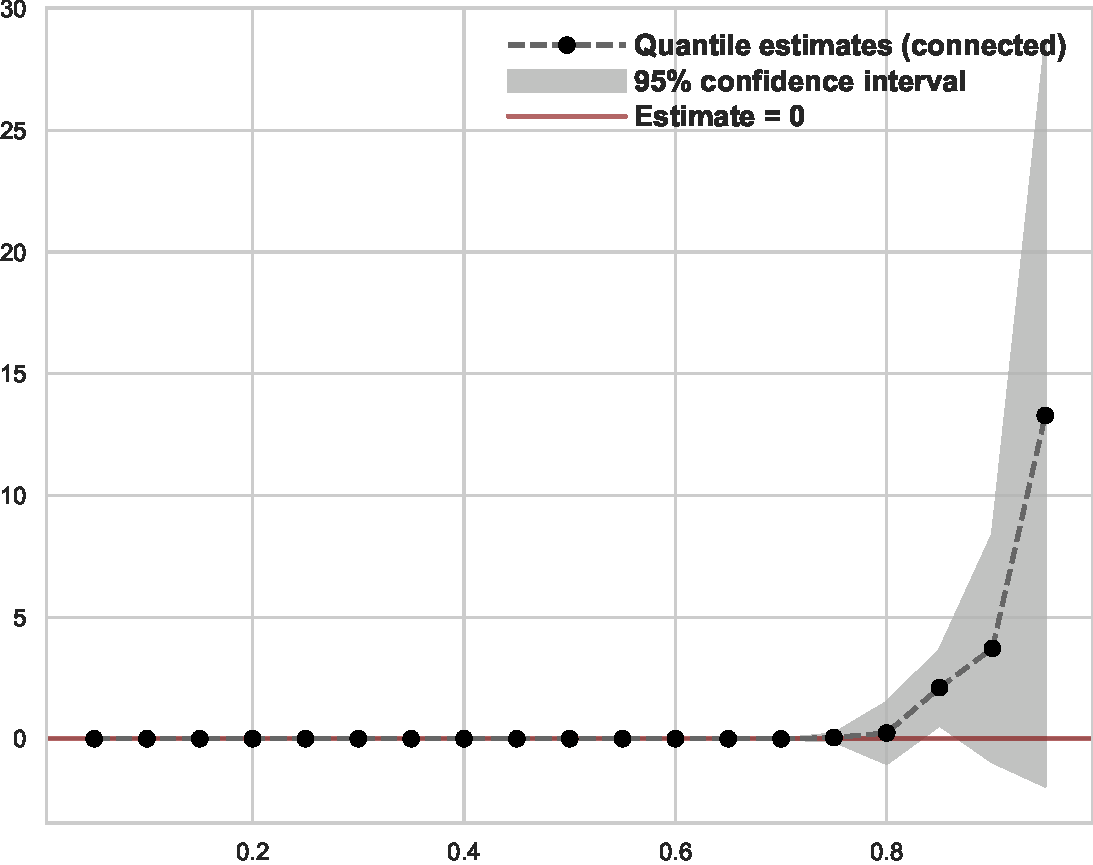
\includegraphics[width=.7\linewidth]{figs/quantile_reg_proportion_duration_adult.pdf}
	\caption*{\footnotesize \emph{Notes:} 
		The dependent variable is the percentage of time individuals in our sample spent on pornographic sites.
		Each point indicates the difference between Republicans and Democrats and corresponds to a quantile regression at the quantile indicated by the x-axis.
		95\% confidence intervals constructed from standard errors.
		See \cref{fig:quantile_regression_prop_duration_covariates} for the same plot controlling for individual characteristics.
            %\cref{tab:quantile-estimates-time} tabulates the estimates.
            \cref{tab:quantile-estimates-time} in \hyperref[sm:smB]{Appendix B} tabulates the estimates.
	}
	\label{fig:quantile_regression_prop_duration}
\end{figure}

Given the skew in the data, we quantify differences in online pornography consumption by party using quantile regression.\footnote{\cref{tab:characteristics_split_by_party_medians} presents non-parametric tests for differences in medians in the consumption of pornography.} Our primary dependent variables of interest are the total time spent on pornographic sites and the proportion of time spent on pornographic sites. We regress the total time (share of time) spent on pornographic sites on an indicator for Republicans. 

As \cref{fig:quantile_regression_duration} shows, the 80th percentile of the difference is close to 0, but from thereon, there is a diverging trend with the 95th percentile difference nearly 1.6 hrs. (\cref{tab:quantile-estimates-hours} reports estimates for each quantile.).\footnote{\hyperref[sm:smF]{Appendix F} describes the distribution of consumption of pornography online by independents. The median independent consumes more pornography than partisans (1.3 hours vs. 0.7 hours in \cref{tab:percentiles_duration_adultsites_by_individuals_independents_partisans} and 3.4\% vs 2.1\% in \cref{tab:percentiles_prop_duration_adultsites_by_individuals_independents_partisans}).}

Looking at the share of time spent on pornographic sites reveals a similar pattern to the one we saw for total time spent (see \cref{fig:quantile_regression_prop_duration}). The 80th percentile of the partisan difference is nearly 0, and after that, the differences rise sharply with differences of more than 2 hours at the 100th percentile (albeit the number is very imprecisely estimated).

Looking at differences in the percentage of partisans who consume any pornographic content, we find little difference. Nearly 31\% percent of Democrats and 30\% percent of Republicans consumed at least some pornography online in June 2022; the difference between the two is not statistically significant (\cref{fig:consume_porn_yes_no}). 

In addition to individual-level demographics, we also have precise timestamps for each visit. We use these timestamps to evaluate the extent to which differences in the timing of consumption differ by partisanship. Overall, we find some evidence that Republicans consume more online pornography in the morning (see \hyperref[sm:smD]{Appendix D}).

\subsection{Accounting for Confounders}

Partisans differ on other characteristics than the party (see \cref{tab:characteristics_split_by_party}). For instance, Democrats are younger (\cref{tab:characteristics_split_by_party}). Add to it that consumers of pornography online tend to be younger (see Panel B of \cref{tab:characteristics_split_by_porn_consumers}). How do differences in age and other such demographic differences between the parties ``explain'' the results? To find out, we control for the following immutable characteristics that predict pornography consumption: age \citep{Wright2013-an, Woodrum1992-vk}, ethnicity \citep{Wright2013-an}, gender \citep{Woodrum1992-vk}, and education level \citep{Woodrum1992-vk}. As \cref{fig:quantile_regression_duration_covariates} and \cref{fig:quantile_regression_prop_duration_covariates} show, once we adjust for confounders, the partisan differences melt away. (For the corresponding table with the various percentiles, see \cref{tab:quantile-estimates-time}.)


%=====================================================
% Fig of quantile regression estimates
% Time Spent on Adult Sites by Party (with covariates) 
%=====================================================
\begin{figure}[!ht]
	\centering
	\caption{Quantile Estimates--Hours Spent on Pornographic Sites by Party (with covariates)}
	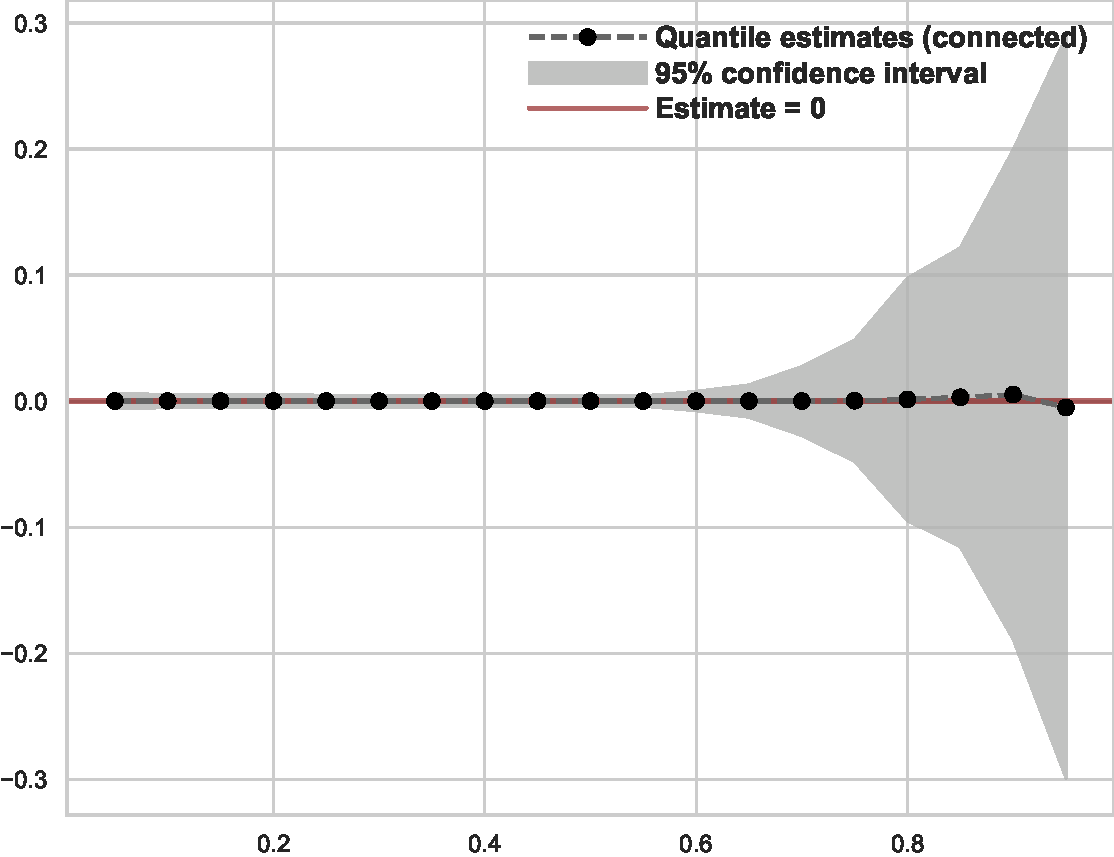
\includegraphics[width=.7\linewidth]{figs/quantile_reg_covariates_duration_adult.pdf}
	\caption*{\footnotesize \emph{Notes:} 
		The dependent variable is the number of hours individuals in our sample spent on pornographic sites.
		Each point indicates the difference between Republicans and Democrats and corresponds to a quantile regression at the quantile indicated by the x-axis.
		Covariates included on the right-hand side are gender (Female/Male), race (White/Black/Hispanic/Asian/Others), education level (no HS/HS graduate/some college/college graduate), age and its quadratic, and region (NE/MW/S/W).
		95\% confidence intervals constructed from standard errors.
		See \cref{fig:quantile_regression_duration} for the same plot without covariates.
  \cref{tab:quantile-estimates-hours} in \hyperref[sm:smB]{Appendix B} tabulates the estimates.
	}
	\label{fig:quantile_regression_duration_covariates}
\end{figure}

%================================================================
% Fig of quantile regression estimates
% Percentage Time Spent on Adult Sites by Party (with covariates) 
%================================================================
\begin{figure}[!ht]
	\centering
	\caption{Quantile Estimates--Percentage of Time Spent on Pornographic Sites by Party (with covariates)}
	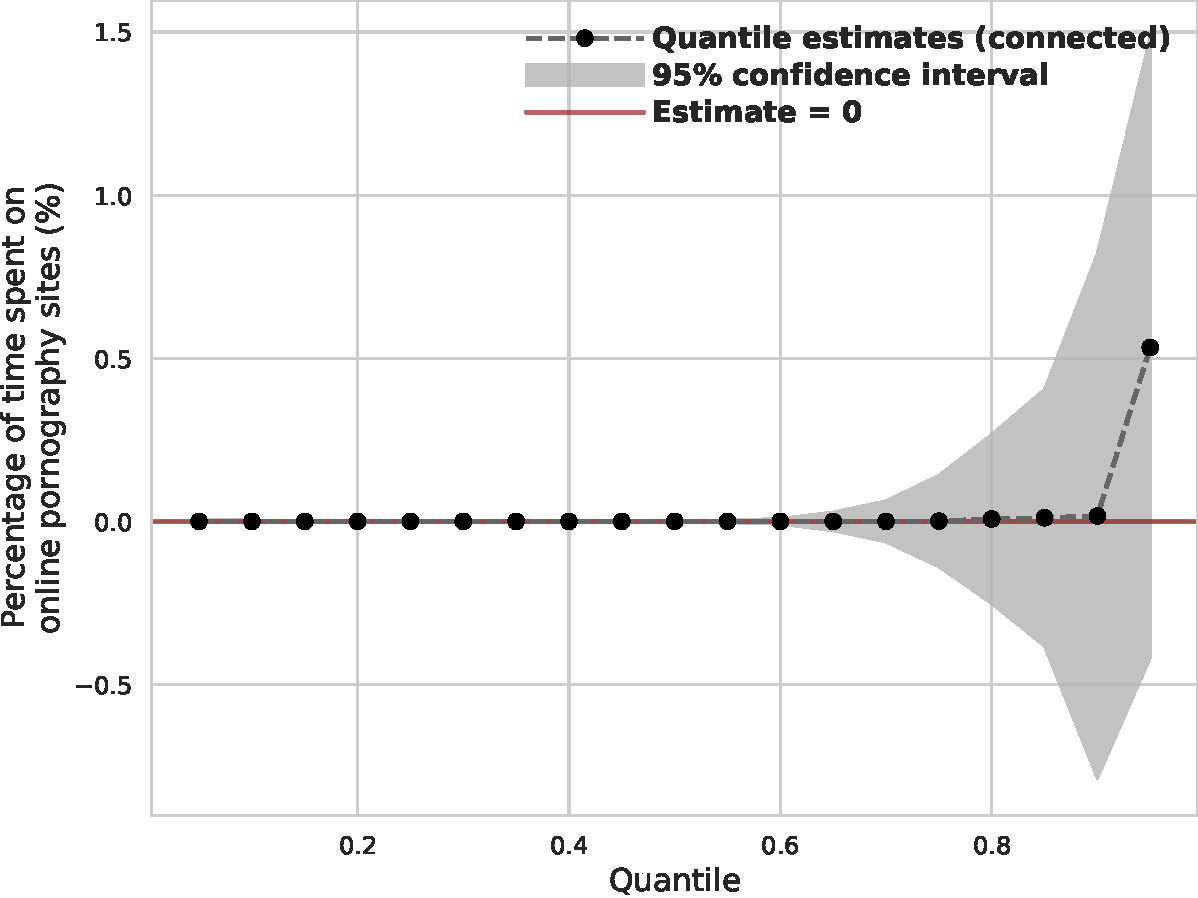
\includegraphics[width=.7\linewidth]{figs/quantile_reg_covariates_proportion_duration_adult.pdf}
	\caption*{\footnotesize \emph{Notes:} 
		The dependent variable is the percentage of time individuals in our sample spent on pornographic sites.
		Each point indicates the difference between Republicans and Democrats and corresponds to a quantile regression at the quantile indicated by the x-axis.
		Covariates included on the right-hand side are: gender (Female/Male), race (White/Black/Hispanic/Asian/Others), education level (no HS/HS graduate/some college/college graduate), age and its quadratic, and region (NE/MW/S/W).
		95\% confidence intervals constructed from standard errors.
		See \cref{fig:quantile_regression_prop_duration} for the same plot without covariates.
        \cref{tab:quantile-estimates-time} in \hyperref[sm:smB]{Appendix B} tabulates the estimates.
	}
	\label{fig:quantile_regression_prop_duration_covariates}
\end{figure}

\subsection{Robustness}
In \ref{si:visits}, we analyze similar metrics for the total number of visits and proportion of visits instead of time. The upshot is that the key conclusions are unaffected (see \cref{tab:distribution_visits_party} and \cref{tab:distribution_prop_visits_party} in \hyperref[sm:smG]{Appendix G}). We also replicate our analyses using four alternative classifications of domains (see \hyperref[sm:smE]{Appendix E}) and obtain similar results. 

\section{Discussion}
\label{sec:discussion}
The consumption of pornography has been attributed to a variety of ills. It is also considered problematic from a religious perspective. For instance, Christian theologians believe that consumption of pornography leads people away from purity and hence should be avoided.\footnote{\url{https://www.churchofjesuschrist.org/study/manual/help-for-pornography-users/effect-of-pornography}} The Internet has dramatically increased access to pornography. This has led to the concern that pornography consumption has become a ``public health crisis''. Our data suggest that pornography consumption online is highly concentrated, with very few people consuming a lot of pornography and most people consuming very little or none.

The paper's primary contribution concerns partisan differences in online pornography consumption. Both parties claim the higher ground when it comes to women—one's case for morality is steeped in religion, the other's in enduring concern for women. We tested this presentiment using individual-level browsing data. The data suggest that partisan differences are likely small.

The key strengths of our unique dataset include having micro-level records of online browsing activities, allowing us to track timestamped visits to online pornography. Moreover, our dataset also allows us to adjust for partisan differences in fundamental baseline demographics.\footnote{Other studies on the topic lack this combination of ground-truth individual-level consumption of online pornography and individual-level demographics (e.g., \cite{Peek1982-ua, Woodrum1992-vk, Markey2011-xo, Perry2020-cp, Ybarra2005-id, Perry2018-cw, Price2016-sm, webporn, Wright2013-gl}).} \footnote{A more subtle strength of our study is that it was conducted around 2022, by which time differences in online content consumption---including pornography content--- are unlikely to be driven by variations in regional broadband penetration, a point \cite{edelman2009markets} worries about.}

Our research has two major limitations. The first concern with our data is that we may not have all the Internet visitation data of a user. If the respondent changes their behavior in response to the knowledge that their data is being collected (even if it is de-identified), for e.g., they may modify their behavior on the machine or figure out ways to evade detection, it may bias our results. In fact, we think it is likely that people would be less likely to search for pornography on machines on which they have installed passive monitoring software (though the data are de-identified). If that is so, our estimates are a lower bound of consumption of online pornography. If this bias varies by party, our estimates of partisan differences will also be biased. 

The second concern is that our measures are a point in time. We have data from one month in one year - June 2022. It is possible that people consume less pornography online and instead spend time outside in June when the weather in many parts of the US is more pleasant than in the preceding or following months. 



%\section{Acknowledgments}
%Acknowledgments/ Author's disclosure/ funding statement.

\bibliography{porn,paperpile}
\addcontentsline{toc}{section}{References}


\clearpage
% =============================================================================
% 	Appendix
% =============================================================================
\setcounter{table}{0}
\setcounter{figure}{0}
\setcounter{equation}{0}

\setcounter{secnumdepth}{0}
\section[Supplementary Information]{\large Supplementary Information}\label{sec:sm}
%\onehalfspacing
\normalsize

\newcommand{\smATitle}{Descriptive Analyses}
\newcommand{\smBTitle}{Partisan Differences}
\newcommand{\smCTitle}{Online Pornography vs. Leisure}
\newcommand{\smDTitle}{Time of Consumption}
\newcommand{\smETitle}{Alternate Classifications of Pornography Sites}
\newcommand{\smFTitle}{Consumption of Pornography Among Independents}
\newcommand{\smGTitle}{Alternate Measures of Pornography}
\newcommand{\smHTitle}{Missing at Random}

%\noindent 
\textbf{\hphantom{aaa}Table of Contents}\\
\hyperref[sm:smA]{\indent \textcolor{magenta}{\S A:}} \smATitle{}\\
\hyperref[sm:smB]{\indent \textcolor{magenta}{\S B:}} \smBTitle{}\\
\hyperref[sm:smC]{\indent \textcolor{magenta}{\S C:}} \smCTitle{}\\
\hyperref[sm:smD]{\indent \textcolor{magenta}{\S D:}} \smDTitle{}\\
\hyperref[sm:smE]{\indent \textcolor{magenta}{\S E:}} \smETitle{}\\
\hyperref[sm:smF]{\indent \textcolor{magenta}{\S F:}} \smFTitle{}\\
\hyperref[sm:smG]{\indent \textcolor{magenta}{\S G:}} \smGTitle{}\\
\hyperref[sm:smH]{\indent \textcolor{magenta}{\S H:}} \smHTitle{}\\

\clearpage
% =============================================================================
\FloatBarrier
\renewcommand{\thetable}{A\arabic{table}}
\renewcommand{\thefigure}{A\arabic{figure}}
\renewcommand{\theequation}{A\arabic{equation}}
\subsection{A. \smATitle{}}\label{sm:smA}
% =============================================================================

\subsubsection{Website Visits Are Highly Skewed}

%================================
% Figure of top 25 non-adultsites
%================================
\begin{figure}[h]
	\centering
	\caption{Top 25 Non-Pornographic Sites}
	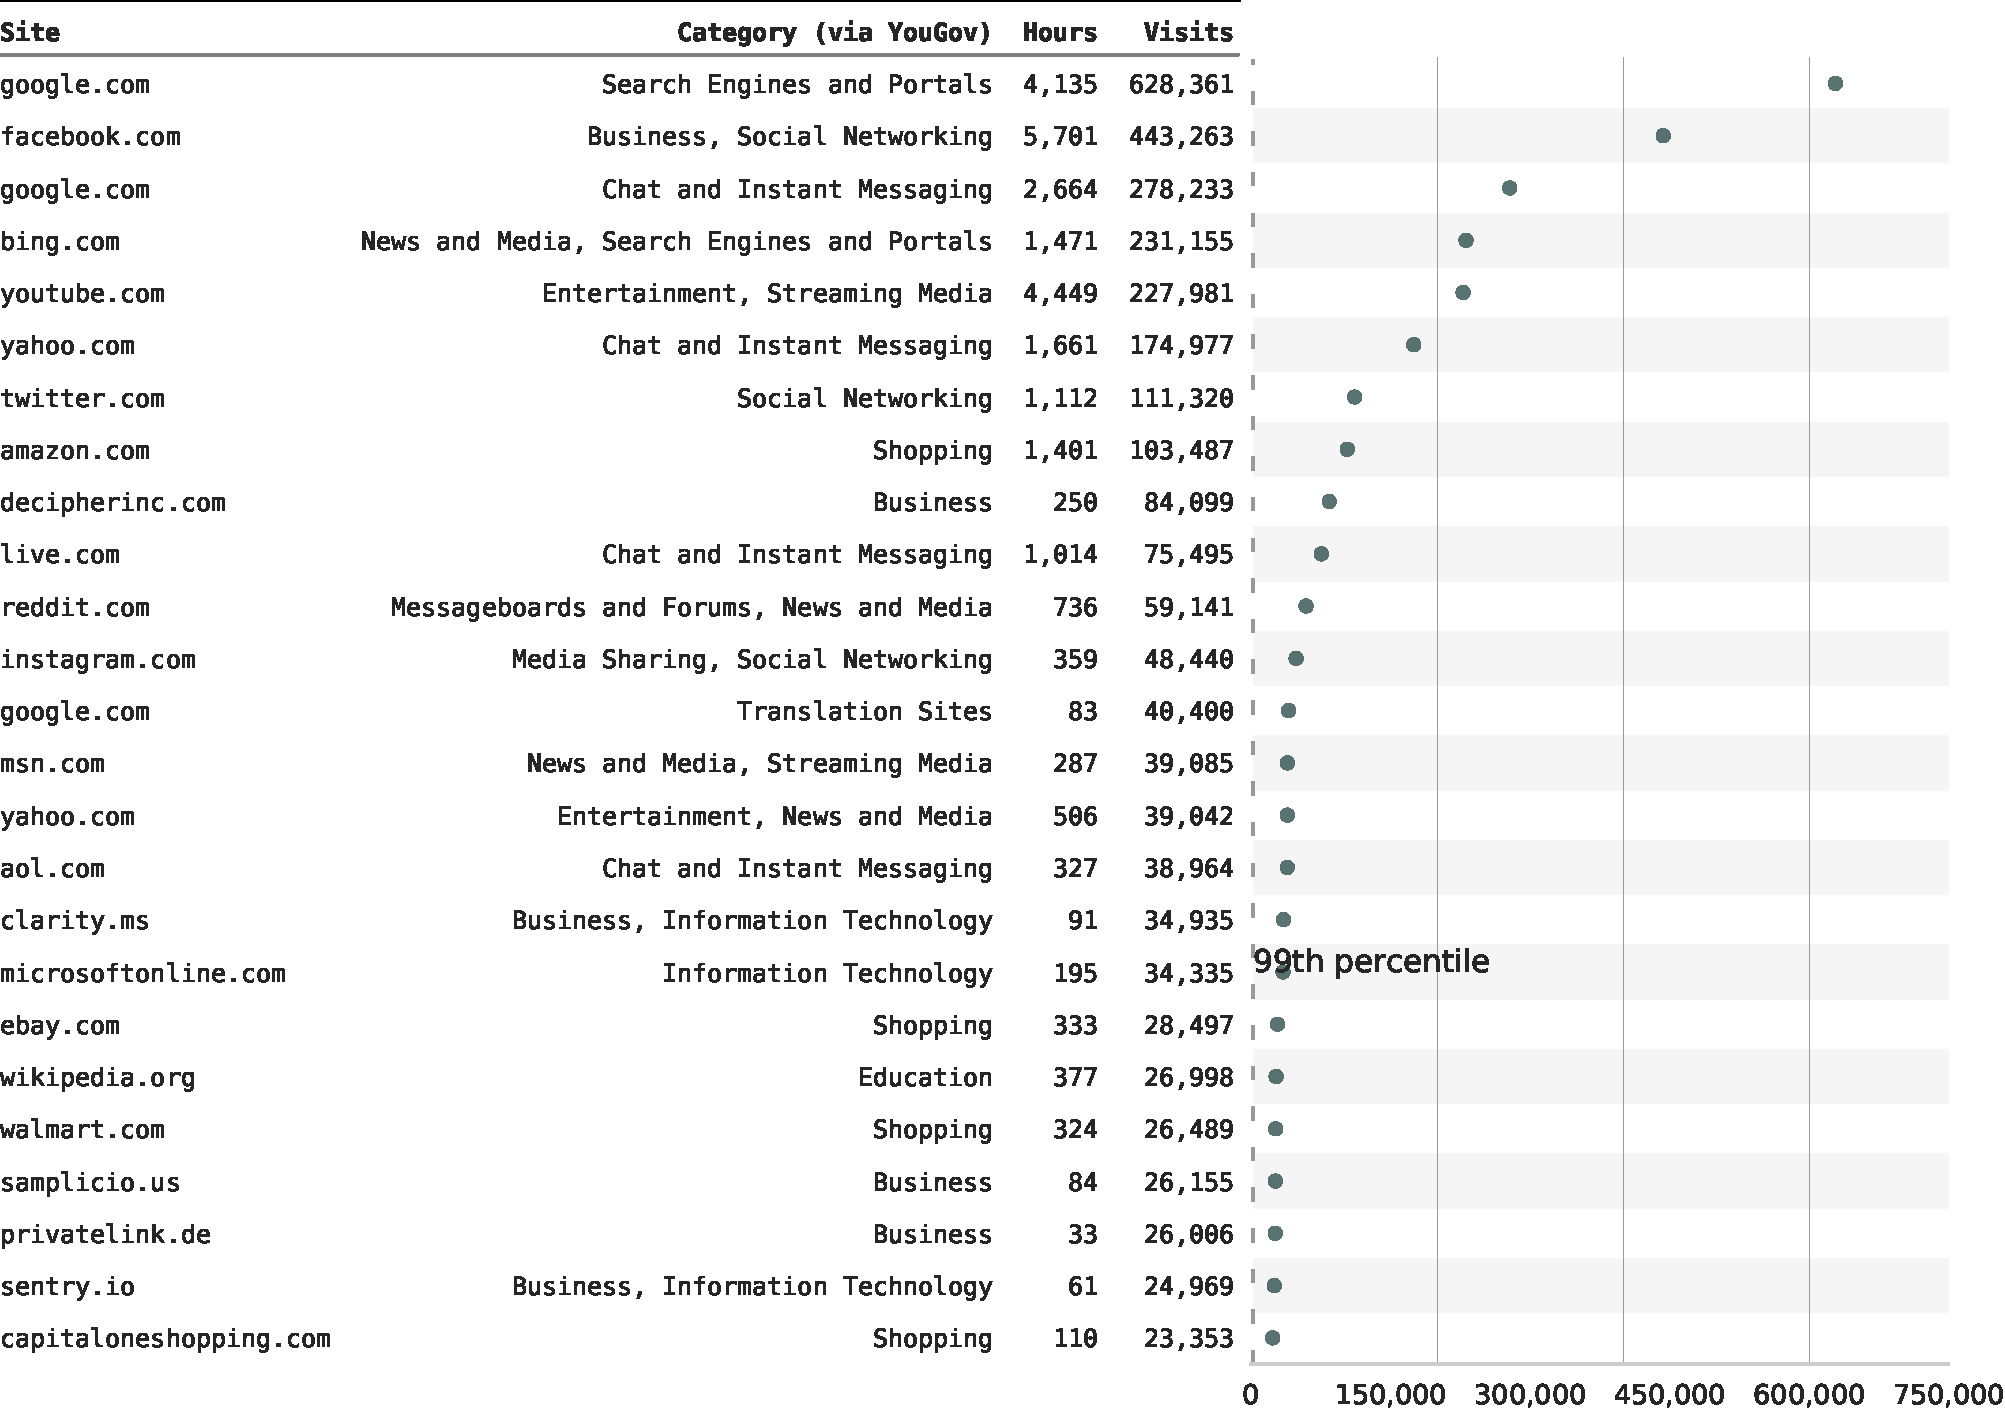
\includegraphics[width=\textwidth]{figs/top_25_nonadultsites.pdf}
	\caption*{\footnotesize \emph{Notes:} 
		The table shows the top 25 non-pornographic sites individuals visited in the sample period.
            All numbers are based on online visits during the one-month period.
		The \emph{Hours} column is the total number of hours individuals in the sample spent on the site. 
		The \emph{Visits} column is the total number of visits by individuals in the sample to the site.  			
		Sites to the right of the vertical dashed are the top 1 percent of non-pornographic sites in visits.
	}
	\label{fig:top25_nonadult}
\end{figure}

%============================
% Figure of top 25 adultsites
%============================
\begin{figure}[ht]
	\centering
	\caption{Top 25 Pornography Sites}
	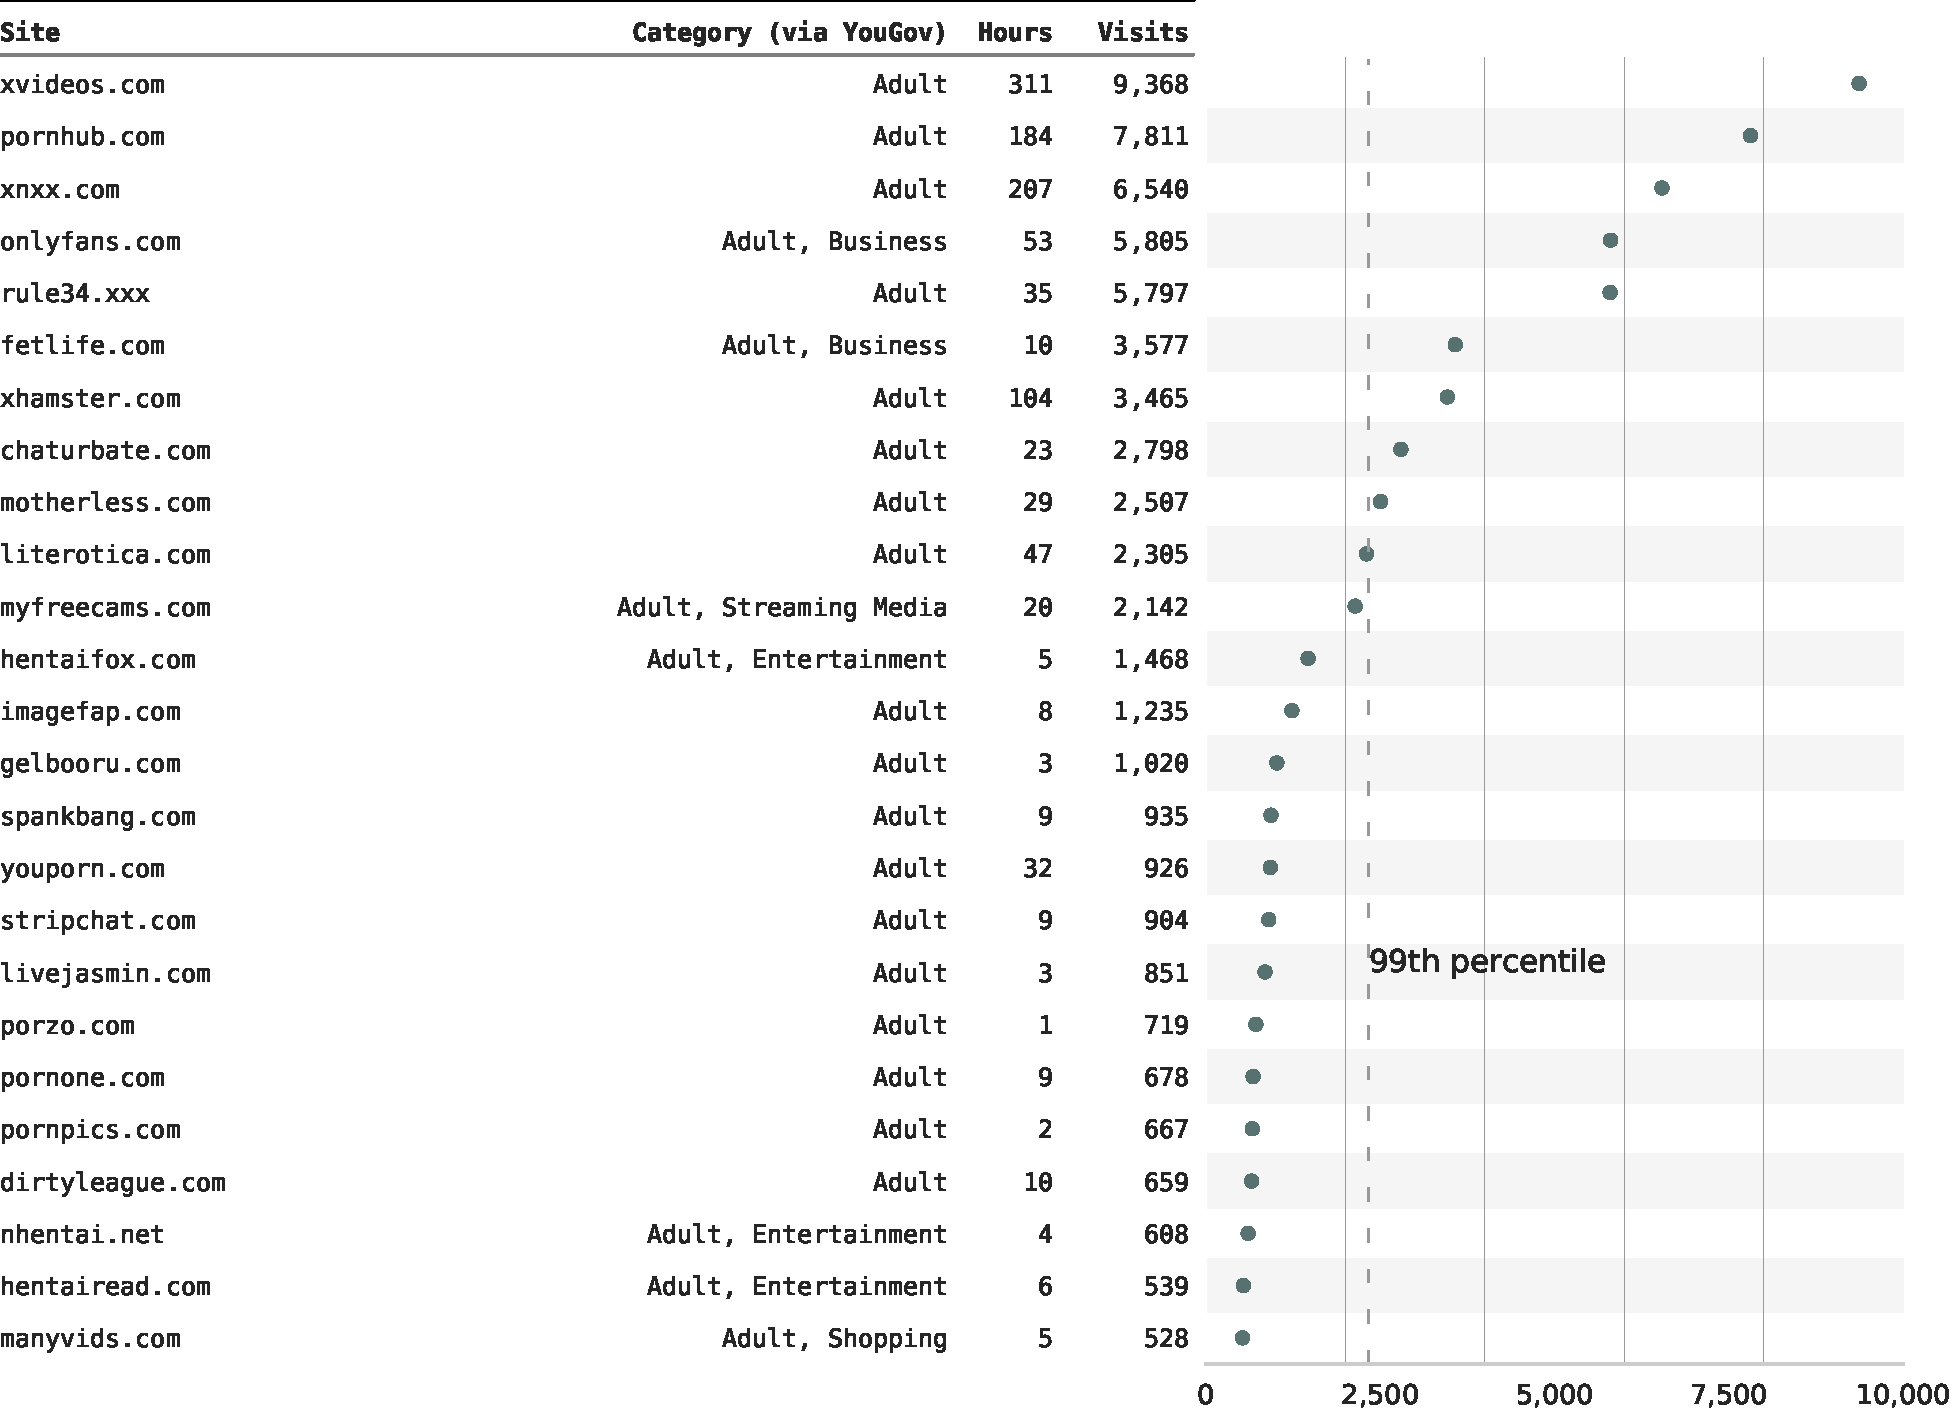
\includegraphics[width=\textwidth]{figs/top_25_adultsites.pdf}
	\caption*{\footnotesize \emph{Notes:} 
		The table shows the top 25 pornographic sites that individuals visited in the sample period.
            All numbers are based on online visits during the one-month period.
		Pornography sites are categorized by YouGov (see the \nameref{sec:data} section).
    	The \emph{Hours} column is the total number of hours individuals in the sample spent on the site. 
    	The \emph{Visits} column is the total number of visits by individuals in the sample to the site.
            Sites to the right of the vertical dashed are the top 1 percent of pornographic sites in visits.
	}
	\label{fig:top25_adult}
\end{figure}



%=============================================
% Figure for concentration of porn consumption
%=============================================
\begin{figure}
	\centering
	\caption{Traffic to Top 10 Pornographic Sites}
	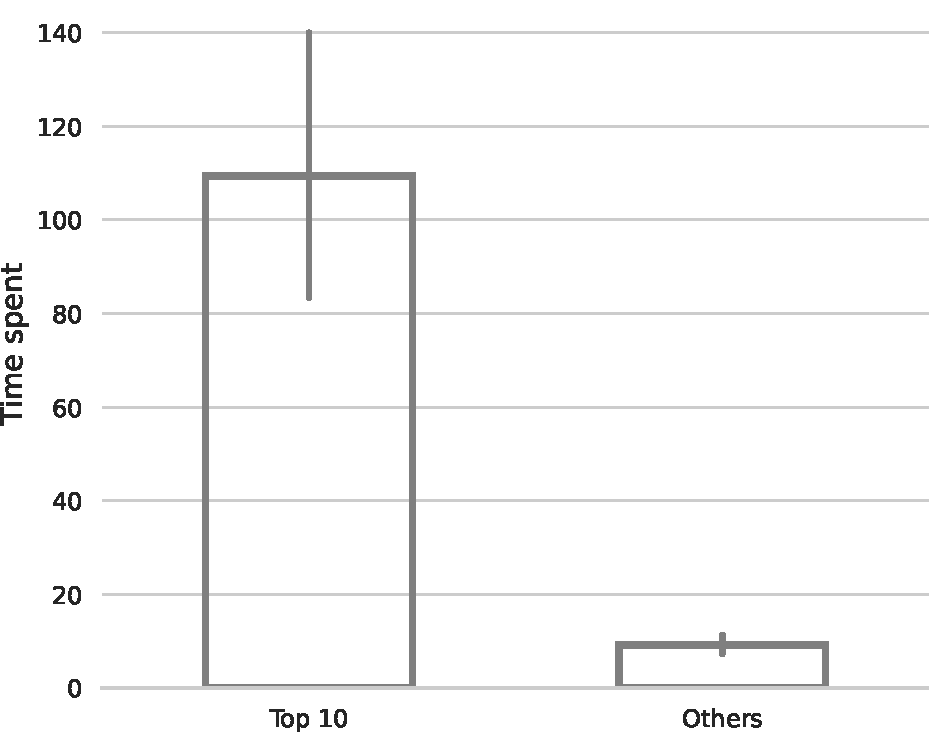
\includegraphics[width=.5\textwidth]{figs/concentration_porn_consumption.pdf}
	\caption*{\footnotesize \emph{Notes:} 
		The Top 10 bar indicates traffic to the top 10 pornographic sites in the data (see \cref{fig:top25_adult}).
		The ``Others'' bar indicates traffic to all other pornographic sites outside of the top 10.
		The y-axis is the total time spent on pornographic sites, averaged across individuals.
		Time units are hours.
		Vertical bars are 95\% confidence intervals from bootstrapped standard errors (n = 1,000).
	}
	\label{fig:concentration_porn_consumption}
\end{figure}

\begin{landscape}% Landscape page
    \begin{table}[ht] \centering \small \setlength\tabcolsep{3 pt} \setlength{\defaultaddspace}{0pt}
    \def\sym#1{\ifmmode^{#1}\else\(^{#1}\)\fi}
    \caption{Time Spent by the Type of Content}
    \label{tab:top10cat_description}
	\begin{adjustbox}{max width=1.325\textwidth}
            \begin{tabular}{@{\hspace{0\tabcolsep}}lrrrrrrrrrrrrrr@{\hspace{0\tabcolsep}}}
            \toprule\toprule
            %\cmidrule(l){2-21}
            &\multicolumn{5}{c}{\textbf{Panel A.} Top sites based on traffic}&\multicolumn{9}{c}{\textbf{Panel B.}}\\
            \cmidrule(lr){2-6}
            &&&\multicolumn{2}{c}{Cumulative}&&\multicolumn{9}{c}{Summary statistics for hours spent on sites}\\
            \cmidrule(l){4-5}\cmidrule{7-15}
            &\multicolumn{1}{c}{Traffic}&\multicolumn{1}{c}{\%}&\multicolumn{1}{c}{Traffic}&\multicolumn{1}{c}{\%}&\multicolumn{1}{c}{Examples of websites}&\multicolumn{1}{c}{Mean}&\multicolumn{1}{c}{S.D.}&\multicolumn{1}{c}{Min}&\multicolumn{1}{c}{p25}&\multicolumn{1}{c}{p50}&\multicolumn{1}{c}{p75}&\multicolumn{1}{c}{p90}&\multicolumn{1}{c}{p95}&\multicolumn{1}{c}{Max}\\
            \cmidrule(l){2-5}
            YouGov category&\multicolumn{1}{c}{(1)}&\multicolumn{1}{c}{(2)}&\multicolumn{1}{c}{(3)}&\multicolumn{1}{c}{(4)}&\multicolumn{1}{c}{(5)}&\multicolumn{1}{c}{(6)}&\multicolumn{1}{c}{(7)}&\multicolumn{1}{c}{(8)}&\multicolumn{1}{c}{(9)}&\multicolumn{1}{c}{(10)}&\multicolumn{1}{c}{(11)}&\multicolumn{1}{c}{(12)}&\multicolumn{1}{c}{(13)}&\multicolumn{1}{c}{(14)} \\
            \midrule
                                              Business & 720,930 & 13.0 &   720,930 & 13.0 & (decipherinc.com, samplicio.us, privatelink.de) & 4.6 &  9.9 & 0.0 & 0.4 & 1.6 & 4.8 & 11.3 & 18.6 & 140.5 \\
                Search Engines and Portals & 670,710 & 12.1 & 1,391,640 & 25.0 &           (google.com, google.co.uk, yahoo.com) & 4.0 &  8.7 & 0.0 & 0.2 & 1.3 & 4.5 & 10.0 & 15.2 & 139.9 \\
                Chat and Instant Messaging & 613,394 & 11.0 & 2,005,034 & 36.0 &               (google.com, yahoo.com, live.com) & 5.9 & 21.3 & 0.0 & 0.0 & 0.2 & 5.3 & 16.4 & 25.1 & 492.3 \\
               Business, Social Networking & 443,281 &  8.0 & 2,448,315 & 44.0 &        (facebook.com, facebook.co, soocial.com) & 5.0 & 16.6 & 0.0 & 0.0 & 0.2 & 2.5 & 11.4 & 23.2 & 245.5 \\
                                  Shopping & 328,300 &  5.9 & 2,776,615 & 49.9 &             (amazon.com, ebay.com, walmart.com) & 3.2 &  7.0 & 0.0 & 0.1 & 0.8 & 3.2 &  8.2 & 14.4 &  79.0 \\
          Business, Information Technology & 284,428 &  5.1 & 3,061,043 & 55.0 &       (clarity.ms, sentry.io, inboxdollars.com) & 1.7 &  4.7 & 0.0 & 0.1 & 0.4 & 1.6 &  3.9 &  6.4 &  87.8 \\
            Entertainment, Streaming Media & 261,165 &  4.7 & 3,322,208 & 59.7 &            (youtube.com, hulu.com, netflix.com) & 5.5 & 28.7 & 0.0 & 0.0 & 0.1 & 1.4 &  9.6 & 20.5 & 617.5 \\
News and Media, Search Engines and Portals & 231,157 &  4.2 & 3,553,365 & 63.9 &                             (bing.com, att.net) & 1.3 &  4.3 & 0.0 & 0.0 & 0.0 & 0.2 &  3.9 &  6.9 &  61.8 \\
                       Business, Education & 181,106 &  3.3 & 3,734,471 & 67.1 &           (yougov.com, google.com, prolific.co) & 1.7 &  4.7 & 0.0 & 0.1 & 0.6 & 1.7 &  3.5 &  6.3 & 104.5 \\
                        Business, Shopping & 135,431 &  2.4 & 3,869,902 & 69.6 &        (amazon.com, rakuten.com, instacart.com) & 1.2 &  3.0 & 0.0 & 0.0 & 0.3 & 1.1 &  3.0 &  5.1 &  32.2 \\       
            \bottomrule
        \end{tabular}
        \end{adjustbox}
        \caption*{\scriptsize
        The table enumerates the top ten categories (YouGov) based on the amount of traffic to the corresponding sites from individuals in the sample.
        Panel A is constructed using the browsing level data (n = 6.3m web browsing records.) Panel B is constructed using the domain-level data (n = 40k).
        }
    \end{table}
\end{landscape}

\FloatBarrier
\subsubsection{Skew in Consumption of Pornographic Content}
%====================================================
% Tabulated percentiles of hours spent on adult sites
%====================================================
\begin{table}[ht] \centering \small \setlength\tabcolsep{10 pt}
	\caption{Distribution of Consumption of Pornography Online (Conditional on having consumed pornography)}
	\label{tab:distribution_duration}
	\begin{adjustbox}{max width=\textwidth}
		\begin{tabular}{cr}
			\toprule
			\multicolumn{1}{c}{\textbf{Percentile}}&\multicolumn{1}{c}{\textbf{Hours}}\\
			\midrule
			0.00 &  0.00 \\
0.10 &  0.02 \\
0.20 &  0.07 \\
0.30 &  0.16 \\
0.40 &  0.33 \\
0.50 &  0.64 \\
0.60 &  1.30 \\
0.70 &  2.20 \\
0.80 &  4.49 \\
0.90 & 10.15 \\
0.95 & 19.50 \\
0.96 & 21.93 \\
0.97 & 27.31 \\
0.98 & 32.22 \\
0.99 & 46.47 \\
1.00 & 93.96 \\\\
			\bottomrule
		\end{tabular}
	\end{adjustbox}
	\caption*{\footnotesize \emph{Notes:} 
		The table shows key percentiles (each of the ten deciles plus quantiles at the right tail) and their corresponding values for the duration (hours) spent by individuals who consumed pornography in the sample period. 
		See \cref{tab:distribution_prop_duration} for the distribution in terms of percentage of time.
		%See \cref{fig:distribution_duration} for the plot.
	}
\end{table}

%=====================================================================
% Tabulated percentiles of the proportion of duration spent on adult sites
%=====================================================================
\begin{table}[ht] \centering \small \setlength\tabcolsep{10 pt}
	\caption{Percentage of Time Spent on Pornographic Sites (Conditional on having consumed pornography)}
	\label{tab:distribution_prop_duration}
	\begin{adjustbox}{max width=\textwidth}
		\begin{tabular}{cr}
			\toprule
			\multicolumn{1}{c}{\textbf{Percentile}}&\multicolumn{1}{c}{\textbf{\% time}}\\
			\midrule
			0.00 &  0.0 \\
0.10 &  0.0 \\
0.20 &  0.1 \\
0.30 &  0.5 \\
0.40 &  1.0 \\
0.50 &  2.4 \\
0.60 &  4.3 \\
0.70 &  7.9 \\
0.80 & 13.5 \\
0.90 & 34.3 \\
0.95 & 55.6 \\
0.96 & 62.8 \\
0.97 & 64.3 \\
0.98 & 68.9 \\
0.99 & 73.9 \\
1.00 & 87.5 \\
			\bottomrule
		\end{tabular}
	\end{adjustbox}
	\caption*{\footnotesize \emph{Notes:} The table shows key percentiles (each of the ten deciles plus quantiles at the right tail) and their corresponding values for the percentage of time on pornography sites spent by individuals who consumed pornography in the sample period. The base number is the individual's own total time spent on the web. See \cref{tab:distribution_duration} for the distribution of total time spent on pornographic websites.}
\end{table}


\clearpage
\setcounter{table}{0}
\setcounter{figure}{0}
\setcounter{equation}{0}
% =============================================================================
\FloatBarrier
\renewcommand{\thetable}{B\arabic{table}}
\renewcommand{\thefigure}{B\arabic{figure}}
\renewcommand{\theequation}{B\arabic{equation}}
\subsection{B. \smBTitle{}}\label{sm:smB}
% =============================================================================

%===========================================================================
% Tabulated splits by party and by percentiles for hours spent on adultsites
%===========================================================================
\begin{table}[ht] \centering \small \setlength\tabcolsep{10 pt}
	\caption{Distribution of Consumption of Pornography Online by Party (Conditional on having consumed pornography)}
	\label{tab:distribution_duration_party}
	\begin{adjustbox}{max width=\textwidth}
		\begin{tabular}{crr}
			\toprule
			\multicolumn{1}{l}{\textbf{}}&\multicolumn{2}{c}{\textbf{Hours}}\\
			\cmidrule(l){2-3}
			\multicolumn{1}{l}{\textbf{Percentile}}&\multicolumn{1}{c}{\textbf{Republicans}}&\multicolumn{1}{c}{\textbf{Democrats}}\\
			\midrule
			0.00 &  0.00 &  0.00 \\
0.10 &  0.04 &  0.02 \\
0.20 &  0.12 &  0.05 \\
0.30 &  0.29 &  0.11 \\
0.40 &  0.58 &  0.18 \\
0.50 &  1.36 &  0.38 \\
0.60 &  2.11 &  0.69 \\
0.70 &  3.04 &  1.37 \\
0.80 &  5.51 &  3.41 \\
0.90 & 11.57 &  7.15 \\
0.95 & 24.91 & 15.57 \\
0.96 & 26.91 & 17.33 \\
0.97 & 27.74 & 19.28 \\
0.98 & 29.30 & 21.65 \\
0.99 & 36.59 & 43.01 \\
1.00 & 37.54 & 90.48 \\\\
			\bottomrule
		\end{tabular}
	\end{adjustbox}
	\caption*{\footnotesize \emph{Notes:} 
		The table shows splits by party and by key percentiles (each of the ten deciles plus quantiles at the right tail) for the duration (hours) spent by individuals who consumed pornography in the sample period. 
		See \cref{tab:distribution_prop_duration_party} for the distribution in terms of percentage of time. 
		A two-sample Kolmogorov–Smirnov test returns a p-value of 0.005, rejecting the null that the Republican and Democrat distributions are the same.
	}
\end{table}

%===============================================================================
% Tabulated splits by party and by percentiles for the proportion of time spent on adultsites
%===============================================================================
\begin{table}[ht] \centering \small \setlength\tabcolsep{10 pt}
	\caption{Percentage of Time Spent on Pornographic Sites by Party (Conditional on having consumed pornography)}
	\label{tab:distribution_prop_duration_party}
	\begin{adjustbox}{max width=\textwidth}
		\begin{tabular}{crr}
			\toprule
			\multicolumn{1}{l}{\textbf{}}&\multicolumn{2}{c}{\textbf{\% time}}\\
			\cmidrule(l){2-3}
			\multicolumn{1}{l}{\textbf{Percentile}}&\multicolumn{1}{c}{\textbf{Republicans}}&\multicolumn{1}{c}{\textbf{Democrats}}\\
			\midrule
			0.00 &  0.0 &  0.0 \\
0.10 &  0.0 &  0.0 \\
0.20 &  0.3 &  0.1 \\
0.30 &  0.8 &  0.2 \\
0.40 &  2.0 &  0.8 \\
0.50 &  3.8 &  1.3 \\
0.60 &  6.4 &  2.6 \\
0.70 & 10.6 &  5.6 \\
0.80 & 20.3 & 11.4 \\
0.90 & 36.3 & 33.3 \\
0.95 & 44.2 & 54.1 \\
0.96 & 52.9 & 56.6 \\
0.97 & 62.3 & 63.4 \\
0.98 & 68.4 & 64.9 \\
0.99 & 71.0 & 72.1 \\
1.00 & 87.5 & 77.4 \\\\
			\bottomrule
		\end{tabular}
	\end{adjustbox}
	\caption*{\footnotesize \emph{Notes:} 
		The table shows splits by party and by key percentiles (each of the ten deciles plus quantiles at the right tail) for the percentage of time spent on pornography by individuals who consumed pornography in the sample period. 
        The base number is the individual's own total time spent on the web.
		See \cref{tab:distribution_duration_party} for the distribution in terms of percentage of time.
		A two-sample Kolmogorov–Smirnov test returns a p-value of 0.025, rejecting the null that the Republican and Democrat distributions are the same at the 5\% level.
		%See \cref{fig:distribution_prop_duration_party} for the plot.
	}
\end{table}

%==============================================================================
% Table for balance of porn consumption and individual characteristics by party
% Difference in medians
%==============================================================================
\begin{table}[ht] \centering \small \setlength\tabcolsep{5 pt}
	\caption{Differences (in Medians) in Pornography Consumption}
	\label{tab:characteristics_split_by_party_medians}
	\begin{adjustbox}{max width=\textwidth}
		\begin{tabular}{@{\hspace{0\tabcolsep}}llrcccrr@{\hspace{0\tabcolsep}}}
			\toprule
			&\multicolumn{7}{c}{\underline{Measures of pornography consumption}}\\
			&\multicolumn{1}{l}{(1)}&\multicolumn{1}{c}{(2)}&\multicolumn{1}{c}{(3)}&\multicolumn{1}{c}{(4)}&\multicolumn{1}{c}{(5)}&\multicolumn{1}{c}{(6)}&\multicolumn{1}{r}{(7)}\\			
			&\multicolumn{1}{l}{Subgroups}&\multicolumn{1}{c}{NA}&\multicolumn{1}{c}{Total}&\multicolumn{1}{c}{Democrats}&\multicolumn{1}{c}{Republicans}&\multicolumn{1}{c}{P-val}&\multicolumn{1}{r}{SMD}\\
			\cmidrule{2-8}
			 n                           &    &           & 1200          & 530           & 356           &           &                 \\
 Minutes, median [Q1,Q3]     &    & 65        & 0.0 [0.0,4.8] & 0.0 [0.0,3.1] & 0.0 [0.0,3.6] & 0.981     & 0.056           \\
 \% of time, median [Q1,Q3]   &    & 65        & 0.0 [0.0,0.1] & 0.0 [0.0,0.1] & 0.0 [0.0,0.1] & 0.842     & 0.049           \\
 Visits, median [Q1,Q3]      &    & 65        & 0.0 [0.0,8.0] & 0.0 [0.0,6.0] & 0.0 [0.0,8.0] & 0.933     & 0.048           \\
 \% of visits, median [Q1,Q3] &    & 65        & 0.0 [0.0,0.2] & 0.0 [0.0,0.1] & 0.0 [0.0,0.2] & 0.916     & 0.085           \\
			\bottomrule
		\end{tabular}
	\end{adjustbox}
	\caption*{\scriptsize \emph{Notes:}
		The table shows splits by party for pornography consumption and for individual characteristics for the 1,200 individuals.
		This table focuses on differences in medians.
		Party identification is based on a 7-point scale. We code 1--3 as ``Democrat'', 4 as ``Independent'', 5--7 as ``Republican''.
		Column (1) shows subgroups for categorical variables.
		Column (2) indicates the count of missing variables, if any.
		Columns (3)--(5) show the medians, the first quartiles, and the third quartiles for the full sample, Democrats, and Republicans.
		1st and 3rd quartiles in brackets.
		Column (6) and column (7) report the p-values and standardized median differences for Democrats vs Republicans.
		See Panel A of \cref{tab:characteristics_split_by_party} for differences in means.
	}
\end{table}
\FloatBarrier
\clearpage
\subsubsection{Accounting for Confounders}

%==============================================================================
% Table for balance of porn consumption and individual characteristics by party
%==============================================================================
\begin{table}[!ht] \centering \ssmall \setlength\tabcolsep{9 pt}
	\caption{Differences in Pornography Consumption and Individual Characteristics by Party}
	\label{tab:characteristics_split_by_party}
	\begin{adjustbox}{max width=\textwidth}
		\begin{tabular}{@{\hspace{0\tabcolsep}}llrcccrr@{\hspace{0\tabcolsep}}}
			\toprule
			&\multicolumn{7}{c}{\underline{Panel A. Measures of pornography consumption}}\\
			&\multicolumn{1}{l}{(1)}&\multicolumn{1}{c}{(2)}&\multicolumn{1}{c}{(3)}&\multicolumn{1}{c}{(4)}&\multicolumn{1}{c}{(5)}&\multicolumn{1}{c}{(6)}&\multicolumn{1}{r}{(7)}\\			
			&\multicolumn{1}{l}{Subgroups}&\multicolumn{1}{c}{NA}&\multicolumn{1}{c}{Total}&\multicolumn{1}{c}{Democrat}&\multicolumn{1}{c}{Republican}&\multicolumn{1}{c}{P-val}&\multicolumn{1}{r}{SMD}\\
			\cmidrule{2-8}
			 n                      &     &           & 1200         & 530          & 356          &           &                 \\
 Consume porn, n (\%)    & No  & 65        & 774 (68.2)   & 343 (68.5)   & 235 (70.6)   & 0.569     & 0.046           \\
                        & Yes &           & 361 (31.8)   & 158 (31.5)   & 98 (29.4)    &           &                 \\
 Minutes, mean (SD)     &     & 65        & 73.4 (342.1) & 58.8 (331.7) & 75.8 (277.4) & 0.423     & 0.056           \\
 \% of time, mean (SD)   &     & 65        & 3.4 (11.2)   & 2.9 (10.7)   & 3.5 (11.1)   & 0.486     & 0.049           \\
 Visits, mean (SD)      &     & 65        & 74.3 (328.9) & 59.9 (298.9) & 73.7 (271.1) & 0.489     & 0.048           \\
 \% of visits, mean (SD) &     & 65        & 2.2 (7.1)    & 1.7 (6.1)    & 2.3 (7.1)    & 0.238     & 0.085           \\
			%-------------------------------------------------------------------
			\cmidrule{2-8}
			&\multicolumn{7}{c}{\underline{Panel B. Individual characteristics}}\\
			&\multicolumn{1}{l}{(1)}&\multicolumn{1}{c}{(2)}&\multicolumn{1}{c}{(3)}&\multicolumn{1}{c}{(4)}&\multicolumn{1}{c}{(5)}&\multicolumn{1}{c}{(6)}&\multicolumn{1}{r}{(7)}\\			
			&\multicolumn{1}{l}{Subgroups}&\multicolumn{1}{c}{NA}&\multicolumn{1}{c}{Total}&\multicolumn{1}{c}{Democrat}&\multicolumn{1}{c}{Republican}&\multicolumn{1}{c}{P-val}&\multicolumn{1}{r}{SMD}\\
			\cmidrule{2-8}
			 n                          &               &           & 1200        & 530         & 356         &           &                 \\
 Party (7-point), mean (SD) &               & 120       & 3.6 (2.2)   & 1.7 (0.8)   & 6.3 (0.8)   & \ensuremath{<}0.001    & 5.670           \\
 2020 Pres. election, n (\%) & Other/No vote & 170       & 270 (26.2)  & 97 (20.2)   & 47 (14.1)   & \ensuremath{<}0.001    & 3.296           \\
                            & Vote Biden    &           & 419 (40.7)  & 369 (76.9)  & 8 (2.4)     &           &                 \\
                            & Vote Trump    &           & 341 (33.1)  & 14 (2.9)    & 278 (83.5)  &           &                 \\
 Age, mean (SD)             &               & 0         & 49.5 (18.1) & 48.7 (17.8) & 55.4 (18.0) & \ensuremath{<}0.001    & 0.373           \\
 Gender, n (\%)              & Female        & 0         & 635 (52.9)  & 312 (58.9)  & 174 (48.9)  & 0.004     & 0.201           \\
                            & Male          &           & 565 (47.1)  & 218 (41.1)  & 182 (51.1)  &           &                 \\
 Race, n (\%)                & Asian         & 0         & 49 (4.1)    & 31 (5.8)    & 6 (1.7)     & \ensuremath{<}0.001    & 0.747           \\
                            & Black         &           & 152 (12.7)  & 96 (18.1)   & 7 (2.0)     &           &                 \\
                            & Hispanic      &           & 176 (14.7)  & 87 (16.4)   & 35 (9.8)    &           &                 \\
                            & Others        &           & 61 (5.1)    & 29 (5.5)    & 9 (2.5)     &           &                 \\
                            & White         &           & 762 (63.5)  & 287 (54.2)  & 299 (84.0)  &           &                 \\
 Education, n (\%)           & College       & 0         & 525 (43.8)  & 258 (48.7)  & 158 (44.4)  & 0.625     & 0.091           \\
                            & HS            &           & 354 (29.5)  & 146 (27.5)  & 103 (28.9)  &           &                 \\
                            & No HS         &           & 73 (6.1)    & 24 (4.5)    & 17 (4.8)    &           &                 \\
                            & Some college  &           & 248 (20.7)  & 102 (19.2)  & 78 (21.9)   &           &                 \\
 Region, n (\%)              & Midwest       & 8         & 239 (20.1)  & 100 (19.0)  & 83 (23.4)   & 0.034     & 0.204           \\
                            & Northeast     &           & 210 (17.6)  & 103 (19.6)  & 50 (14.1)   &           &                 \\
                            & South         &           & 502 (42.1)  & 208 (39.6)  & 159 (44.8)  &           &                 \\
                            & West          &           & 241 (20.2)  & 114 (21.7)  & 63 (17.7)   &           &                 \\
			\bottomrule
		\end{tabular}
	\end{adjustbox}
	\caption*{\scriptsize \emph{Notes:}
		The table shows splits by party for pornographic consumption and for individual characteristics for the 1,200 individuals.
		Party identification is based on a 7-point scale. We code 1--3 as ``Democrat'', 4 as ``Independent'', 5--7 as ``Republican''.
		Column (1) shows subgroups for categorical variables.
		Column (2) indicates the count of missing variables, if any.
		Columns (3)--(5) show means and standard deviations for continuous variables and count and percentage of data for categorical variables for the full sample, Democratic individuals, and Republican individuals.
		Standard deviations and percentages are in parentheses.
		Column (6) and column (7) report the p-values and standardized mean differences for Democrats vs Republicans.
		Given the skew in consumption of pornography, we also performed tests for differences in medians for the measures of pornography consumption by party (see \cref{tab:characteristics_split_by_party_medians}).
	}
\end{table}


%==============================================================================
% Table for balance of porn consumption and individual characteristics by consumer
%==============================================================================
\begin{table}[ht] \centering \scriptsize \setlength\tabcolsep{6 pt}
	\caption{Differences in Pornography Consumption and Individual Characteristics by Pornography Consumers}
	\label{tab:characteristics_split_by_porn_consumers}
	\begin{adjustbox}{max width=\textwidth}
		\begin{tabular}{@{\hspace{0\tabcolsep}}llrcccrr@{\hspace{0\tabcolsep}}}
			\toprule
			&\multicolumn{7}{c}{\underline{Panel A. Measures of pornography consumption}}\\
			&\multicolumn{1}{l}{(1)}&\multicolumn{1}{c}{(2)}&\multicolumn{1}{c}{(3)}&\multicolumn{1}{c}{(4)}&\multicolumn{1}{c}{(5)}&\multicolumn{1}{c}{(6)}&\multicolumn{1}{r}{(7)}\\			
			&\multicolumn{1}{l}{Subgroups}&\multicolumn{1}{c}{NA}&\multicolumn{1}{c}{Total}&\multicolumn{1}{c}{Non-Consumers}&\multicolumn{1}{c}{Consumers}&\multicolumn{1}{c}{P-val}&\multicolumn{1}{r}{SMD}\\
			\cmidrule{2-8}
			 n                      &    &           & 1200         & 774       & 361           &           &                \\
 Minutes, mean (SD)     &    & 65        & 73.4 (342.1) & 0.0 (0.0) & 230.8 (576.3) & \ensuremath{<}0.001    & 0.566          \\
 \% of time, mean (SD)   &    & 65        & 3.4 (11.2)   & 0.0 (0.0) & 10.6 (17.9)   & \ensuremath{<}0.001    & 0.833          \\
 Visits, mean (SD)      &    & 65        & 74.3 (328.9) & 0.0 (0.0) & 233.5 (550.8) & \ensuremath{<}0.001    & 0.599          \\
 \% of visits, mean (SD) &    & 65        & 2.2 (7.1)    & 0.0 (0.0) & 6.9 (11.2)    & \ensuremath{<}0.001    & 0.870          \\
			%-------------------------------------------------------------------
			\cmidrule{2-8}
			&\multicolumn{7}{c}{\underline{Panel B. Individual characteristics}}\\
			&\multicolumn{1}{l}{(1)}&\multicolumn{1}{c}{(2)}&\multicolumn{1}{c}{(3)}&\multicolumn{1}{c}{(4)}&\multicolumn{1}{c}{(5)}&\multicolumn{1}{c}{(6)}&\multicolumn{1}{r}{(7)}\\			
			&\multicolumn{1}{l}{Subgroups}&\multicolumn{1}{c}{NA}&\multicolumn{1}{c}{Total}&\multicolumn{1}{c}{Non-Consumers}&\multicolumn{1}{c}{Consumers}&\multicolumn{1}{c}{P-val}&\multicolumn{1}{r}{SMD}\\
			\cmidrule{2-8}
			 n                          &               &           & 1200        & 774         & 361         &           &                \\
 Party (7-point), mean (SD) &               & 120       & 3.6 (2.2)   & 3.6 (2.2)   & 3.6 (2.1)   & 0.580     & -0.037         \\
 2020 Pres. election, n (\%) & Other/No vote & 170       & 270 (26.2)  & 145 (22.1)  & 110 (34.9)  & \ensuremath{<}0.001    & 0.287          \\
                            & Vote Biden    &           & 419 (40.7)  & 281 (42.8)  & 114 (36.2)  &           &                \\
                            & Vote Trump    &           & 341 (33.1)  & 230 (35.1)  & 91 (28.9)   &           &                \\
 Age, mean (SD)             &               & 0         & 49.5 (18.1) & 51.3 (18.2) & 46.1 (17.1) & \ensuremath{<}0.001    & -0.295         \\
 Gender, n (\%)              & Female        & 0         & 635 (52.9)  & 487 (62.9)  & 109 (30.2)  & \ensuremath{<}0.001    & 0.695          \\
                            & Male          &           & 565 (47.1)  & 287 (37.1)  & 252 (69.8)  &           &                \\
 Race, n (\%)                & Asian         & 0         & 49 (4.1)    & 37 (4.8)    & 9 (2.5)     & 0.059     & 0.193          \\
                            & Black         &           & 152 (12.7)  & 86 (11.1)   & 58 (16.1)   &           &                \\
                            & Hispanic      &           & 176 (14.7)  & 113 (14.6)  & 55 (15.2)   &           &                \\
                            & Others        &           & 61 (5.1)    & 36 (4.7)    & 20 (5.5)    &           &                \\
                            & White         &           & 762 (63.5)  & 502 (64.9)  & 219 (60.7)  &           &                \\
 Education, n (\%)           & College       & 0         & 525 (43.8)  & 363 (46.9)  & 131 (36.3)  & 0.002     & 0.244          \\
                            & HS            &           & 354 (29.5)  & 228 (29.5)  & 115 (31.9)  &           &                \\
                            & No HS         &           & 73 (6.1)    & 46 (5.9)    & 22 (6.1)    &           &                \\
                            & Some college  &           & 248 (20.7)  & 137 (17.7)  & 93 (25.8)   &           &                \\
 Region, n (\%)              & Midwest       & 8         & 239 (20.1)  & 147 (19.2)  & 78 (21.7)   & 0.659     & 0.081          \\
                            & Northeast     &           & 210 (17.6)  & 140 (18.3)  & 60 (16.7)   &           &                \\
                            & South         &           & 502 (42.1)  & 328 (42.8)  & 146 (40.6)  &           &                \\
                            & West          &           & 241 (20.2)  & 152 (19.8)  & 76 (21.1)   &           &                \\
			\bottomrule
		\end{tabular}
	\end{adjustbox}
	\caption*{\scriptsize \emph{Notes:}
		The table shows splits by consumers of pornography for pornography consumption and for individual characteristics for the 1,200 individuals.
		65 of the 1,200 individuals did not clock any browsing activity and are in the first panel.
		These 65 individuals are not substantially different in characteristics than those included in the sample (untabulated).
		Party identification is based on a 7-point scale. We code 1--3 as ``Democrat'', 4 as ``Independent'', 5--7 as ``Republican''.
		Column (1) shows subgroups for categorical variables.
		Column (2) indicates the count of missing variables, if any.
		Columns (3)--(5) show means and standard deviations for continuous variables and count and percentage of data for categorical variables, for the full sample, non-consumers of pornography, and consumers of pornography.
		Standard deviations and percentages are in parentheses.
		Column (6) and column (7) report the p-values and standardized mean differences for non-consumers vs consumers.
	}
\end{table}




\clearpage

\begin{landscape}% Landscape page
    \begin{table}[ht] \centering \ssmall \setlength\tabcolsep{0 pt} \setlength{\defaultaddspace}{0pt}
    \def\sym#1{\ifmmode^{#1}\else\(^{#1}\)\fi}
    \caption{Quantile Estimates--Hours spent on Pornographic Sites by Party }
    \label{tab:quantile-estimates-hours}
	\begin{adjustbox}{max width=1.325\textwidth}
            \begin{tabular}{l*{20}{D{.}{.}{-1}}}
            \toprule\toprule
            &\multicolumn{1}{c}{(1)}         &\multicolumn{1}{c}{(2)}         &\multicolumn{1}{c}{(3)}         &\multicolumn{1}{c}{(4)}         &\multicolumn{1}{c}{(5)}         &\multicolumn{1}{c}{(6)}         &\multicolumn{1}{c}{(7)}         &\multicolumn{1}{c}{(8)}         &\multicolumn{1}{c}{(9)}         &\multicolumn{1}{c}{(10)}&\multicolumn{1}{c}{(11)}         &\multicolumn{1}{c}{(12)}         &\multicolumn{1}{c}{(13)}         &\multicolumn{1}{c}{(14)}         &\multicolumn{1}{c}{(15)}         &\multicolumn{1}{c}{(16)}         &\multicolumn{1}{c}{(17)}         &\multicolumn{1}{c}{(18)}         &\multicolumn{1}{c}{(19)}         &\multicolumn{1}{c}{(20)}         \\
            \cmidrule(l){2-21}
            % ===================================================================
            % Panel A
            &\multicolumn{20}{c}{\textbf{Panel A. Unconditional quantile estimates}}\\
            &\multicolumn{1}{c}{p5}         &\multicolumn{1}{c}{p10}         &\multicolumn{1}{c}{p15}         &\multicolumn{1}{c}{p20}         &\multicolumn{1}{c}{p25}         &\multicolumn{1}{c}{p30}         &\multicolumn{1}{c}{p35}         &\multicolumn{1}{c}{p40}         &\multicolumn{1}{c}{p45}         &\multicolumn{1}{c}{p50}&\multicolumn{1}{c}{p55}         &\multicolumn{1}{c}{p60}         &\multicolumn{1}{c}{p65}         &\multicolumn{1}{c}{p70}         &\multicolumn{1}{c}{p75}         &\multicolumn{1}{c}{p80}         &\multicolumn{1}{c}{p85}         &\multicolumn{1}{c}{p90}         &\multicolumn{1}{c}{p95}         &\multicolumn{1}{c}{p100}         \\
            \cmidrule(l){2-21}
             Republican & 0.28 & -0.00 & -0.00 & -0.00 & -0.00 & -0.00 & -0.00 & -0.00 & -0.00 & -0.00 & -0.00 & -0.00 & -0.00 & -0.00 & -0.00\sym{a} & 0.01 & 0.17 & 0.80\sym{a} & 1.61\sym{a} & 2.10 \\
& (0.35) & (0.00) & (0.00) & (0.00) & (0.00) & (0.00) & (0.00) & (0.00) & (0.00) & (0.00) & (0.00) & (0.00) & (0.00) & (0.00) & (0.00) & (0.04) & (0.11) & (0.30) & (0.49) & (1.84) \\
 Constant & 0.98\sym{a} & 0.00 & 0.00 & 0.00 & 0.00 & 0.00 & 0.00 & 0.00 & 0.00 & 0.00 & 0.00 & 0.00 & 0.00 & 0.00 & 0.00\sym{a} & 0.05\sym{c} & 0.16\sym{b} & 0.49\sym{b} & 1.01\sym{a} & 4.52\sym{a} \\
& (0.25) & (0.00) & (0.00) & (0.00) & (0.00) & (0.00) & (0.00) & (0.00) & (0.00) & (0.00) & (0.00) & (0.00) & (0.00) & (0.00) & (0.00) & (0.03) & (0.07) & (0.19) & (0.31) & (1.17) \\
            \cmidrule(l){2-21}
            % ===================================================================
            % Panel B            
            &\multicolumn{20}{c}{\textbf{Panel B. Adjusted quantile estimates}}\\
            &\multicolumn{1}{c}{p5}         &\multicolumn{1}{c}{p10}         &\multicolumn{1}{c}{p15}         &\multicolumn{1}{c}{p20}         &\multicolumn{1}{c}{p25}         &\multicolumn{1}{c}{p30}         &\multicolumn{1}{c}{p35}         &\multicolumn{1}{c}{p40}         &\multicolumn{1}{c}{p45}         &\multicolumn{1}{c}{p50}&\multicolumn{1}{c}{p55}         &\multicolumn{1}{c}{p60}         &\multicolumn{1}{c}{p65}         &\multicolumn{1}{c}{p70}         &\multicolumn{1}{c}{p75}         &\multicolumn{1}{c}{p80}         &\multicolumn{1}{c}{p85}         &\multicolumn{1}{c}{p90}         &\multicolumn{1}{c}{p95}         &\multicolumn{1}{c}{p100}         \\  
            \cmidrule(l){2-21}
              Republican & 0.17 & -0.00 & -0.00 & -0.00 & -0.00 & -0.00 & -0.00 & -0.00 & -0.00 & -0.00 & -0.00 & -0.00 & 0.00 & 0.00 & 0.00 & 0.00 & 0.00 & 0.00 & 0.01 & 0.02 \\
& (0.29) & (0.00) & (0.00) & (0.00) & (0.00) & (0.00) & (0.00) & (0.00) & (0.00) & (0.00) & (0.00) & (0.00) & (0.00) & (0.01) & (0.01) & (0.02) & (0.04) & (0.05) & (0.09) & (0.14) \\
 Female & -1.56\sym{a} & -0.00 & -0.00 & -0.00 & -0.00 & -0.00 & -0.00 & -0.00 & -0.00 & -0.00 & -0.00 & -0.01\sym{a} & -0.06\sym{a} & -0.17\sym{a} & -0.36\sym{a} & -0.73\sym{a} & -1.53\sym{a} & -2.32\sym{a} & -4.26\sym{a} & -9.40\sym{a} \\
& (0.37) & (0.00) & (0.00) & (0.00) & (0.00) & (0.00) & (0.00) & (0.00) & (0.00) & (0.00) & (0.00) & (0.00) & (0.00) & (0.01) & (0.01) & (0.02) & (0.04) & (0.05) & (0.08) & (0.14) \\
 Educ (HS) & 0.85\sym{b} & 0.00 & 0.00 & 0.00 & 0.00 & 0.00 & 0.00 & 0.00 & 0.00 & 0.00 & 0.00 & 0.00 & 0.00 & 0.00 & 0.00 & 0.00 & 0.00 & 0.01 & 0.02 & 0.12 \\
& (0.33) & (0.00) & (0.00) & (0.00) & (0.00) & (0.00) & (0.00) & (0.00) & (0.00) & (0.00) & (0.00) & (0.00) & (0.01) & (0.01) & (0.03) & (0.05) & (0.09) & (0.13) & (0.22) & (0.40) \\
 Educ (some coll.) & 1.58\sym{b} & 0.00 & 0.00 & 0.00 & 0.00 & 0.00 & 0.00 & 0.00 & 0.00 & 0.00 & 0.00 & 0.00 & 0.00 & 0.00 & 0.00 & 0.02 & 0.05 & 0.29\sym{b} & 0.47\sym{b} & 4.61\sym{a} \\
& (0.64) & (0.00) & (0.00) & (0.00) & (0.00) & (0.00) & (0.00) & (0.00) & (0.00) & (0.00) & (0.00) & (0.00) & (0.01) & (0.01) & (0.03) & (0.05) & (0.10) & (0.14) & (0.22) & (0.41) \\
 Educ (coll. grad.) & 0.42\sym{b} & -0.00 & -0.00 & -0.00 & -0.00 & -0.00 & -0.00 & -0.00 & -0.00 & 0.00 & 0.00 & 0.00 & 0.00 & 0.00 & 0.00 & 0.00 & 0.00 & 0.00 & 0.00 & 0.03 \\
& (0.20) & (0.00) & (0.00) & (0.00) & (0.00) & (0.00) & (0.00) & (0.00) & (0.00) & (0.00) & (0.00) & (0.00) & (0.01) & (0.01) & (0.03) & (0.05) & (0.09) & (0.13) & (0.21) & (0.39) \\
 Age & 0.08 & -0.00 & -0.00 & -0.00 & -0.00 & -0.00 & -0.00 & -0.00 & -0.00 & -0.00 & -0.00 & -0.00 & -0.00 & -0.00 & -0.00 & -0.00 & -0.01 & -0.02\sym{b} & -0.03\sym{b} & -0.01 \\
& (0.05) & (0.00) & (0.00) & (0.00) & (0.00) & (0.00) & (0.00) & (0.00) & (0.00) & (0.00) & (0.00) & (0.00) & (0.00) & (0.00) & (0.00) & (0.00) & (0.01) & (0.01) & (0.01) & (0.02) \\
 Age$^2$ & -0.00\sym{c} & 0.00 & -0.00 & -0.00 & -0.00 & -0.00 & -0.00 & -0.00 & -0.00 & -0.00 & 0.00 & 0.00 & 0.00 & 0.00 & 0.00 & 0.00 & 0.00 & 0.00\sym{c} & 0.00\sym{c} & 0.00 \\
& (0.00) & (0.00) & (0.00) & (0.00) & (0.00) & (0.00) & (0.00) & (0.00) & (0.00) & (0.00) & (0.00) & (0.00) & (0.00) & (0.00) & (0.00) & (0.00) & (0.00) & (0.00) & (0.00) & (0.00) \\
 Race (Black) & 0.63 & 0.00 & 0.00 & 0.00 & 0.00 & 0.00 & 0.00 & 0.00 & 0.00 & 0.00 & 0.00 & 0.00 & 0.00 & 0.00 & 0.00 & 0.00 & 0.00 & 0.00 & 0.04 & 4.31\sym{a} \\
& (0.76) & (0.00) & (0.00) & (0.00) & (0.00) & (0.00) & (0.00) & (0.00) & (0.00) & (0.00) & (0.00) & (0.00) & (0.00) & (0.01) & (0.02) & (0.03) & (0.06) & (0.09) & (0.14) & (0.24) \\
 Race (Hispanic) & 0.26 & 0.00 & 0.00 & 0.00 & 0.00 & 0.00 & 0.00 & 0.00 & 0.00 & 0.00 & 0.00 & 0.00 & -0.00 & -0.00 & -0.00 & 0.00 & 0.05 & 0.04 & 0.01 & 0.58\sym{a} \\
& (0.74) & (0.00) & (0.00) & (0.00) & (0.00) & (0.00) & (0.00) & (0.00) & (0.00) & (0.00) & (0.00) & (0.00) & (0.00) & (0.01) & (0.02) & (0.03) & (0.06) & (0.07) & (0.12) & (0.21) \\
 Race (Asian) & -0.40 & -0.00 & -0.00 & -0.00 & -0.00 & -0.00 & -0.00 & -0.00 & -0.00 & -0.00 & -0.00 & -0.00 & -0.00 & -0.00 & -0.00 & 0.00 & -0.00 & -0.02 & -0.03 & -0.09 \\
& (0.51) & (0.00) & (0.00) & (0.00) & (0.00) & (0.00) & (0.00) & (0.00) & (0.00) & (0.00) & (0.00) & (0.00) & (0.01) & (0.01) & (0.03) & (0.05) & (0.10) & (0.13) & (0.25) & (0.48) \\
 Race (Other) & 0.28 & 0.00 & 0.00 & 0.00 & 0.00 & 0.00 & 0.00 & 0.00 & 0.00 & 0.00 & 0.00 & 0.00 & 0.00 & 0.03\sym{b} & 0.18\sym{a} & 0.63\sym{a} & 0.26\sym{a} & 0.03 & 0.84\sym{a} & 1.39\sym{a} \\
& (0.48) & (0.00) & (0.00) & (0.00) & (0.00) & (0.00) & (0.00) & (0.00) & (0.00) & (0.00) & (0.00) & (0.00) & (0.01) & (0.01) & (0.03) & (0.05) & (0.10) & (0.13) & (0.22) & (0.38) \\
 Region (MW) & 1.26\sym{b} & 0.00 & 0.00 & 0.00 & 0.00 & 0.00 & 0.00 & 0.00 & 0.00 & 0.00 & 0.00 & 0.01\sym{c} & 0.06\sym{a} & 0.17\sym{a} & 0.18\sym{a} & 0.63\sym{a} & 0.32 & 0.00 & 0.01 & 0.45 \\
& (0.60) & (0.01) & (0.01) & (0.01) & (0.01) & (0.01) & (0.01) & (0.01) & (0.01) & (0.01) & (0.01) & (0.01) & (0.01) & (0.03) & (0.07) & (0.13) & (0.27) & (0.31) & (0.60) & (1.43) \\
 Region (South) & 1.00\sym{c} & 0.00 & 0.00 & 0.00 & 0.00 & 0.00 & 0.00 & 0.00 & 0.00 & 0.00 & 0.00 & 0.01\sym{c} & 0.06\sym{a} & 0.17\sym{a} & 0.18\sym{a} & 0.63\sym{a} & 0.33 & 0.00 & 0.01 & 0.10 \\
& (0.58) & (0.01) & (0.01) & (0.01) & (0.01) & (0.01) & (0.01) & (0.01) & (0.01) & (0.01) & (0.01) & (0.01) & (0.01) & (0.03) & (0.07) & (0.13) & (0.27) & (0.31) & (0.60) & (1.43) \\
 Region (West) & 1.43\sym{b} & 0.00 & 0.00 & 0.00 & 0.00 & 0.00 & 0.00 & 0.00 & 0.00 & 0.00 & 0.00 & 0.01\sym{c} & 0.06\sym{a} & 0.17\sym{a} & 0.18\sym{a} & 0.63\sym{a} & 0.36 & 0.01 & 0.42 & 0.13 \\
& (0.58) & (0.01) & (0.01) & (0.01) & (0.01) & (0.01) & (0.01) & (0.01) & (0.01) & (0.01) & (0.01) & (0.01) & (0.01) & (0.03) & (0.07) & (0.13) & (0.27) & (0.31) & (0.60) & (1.43) \\
 Constant & -1.67 & 0.00 & 0.00 & 0.00 & 0.00 & 0.00 & 0.00 & 0.00 & 0.00 & 0.00 & 0.00 & 0.00 & 0.00 & 0.00 & 0.18\sym{b} & 0.10 & 1.43\sym{a} & 2.99\sym{a} & 5.32\sym{a} & 9.64\sym{a} \\
& (1.25) & (0.01) & (0.01) & (0.01) & (0.01) & (0.01) & (0.01) & (0.01) & (0.01) & (0.01) & (0.01) & (0.01) & (0.02) & (0.04) & (0.08) & (0.15) & (0.30) & (0.36) & (0.66) & (1.51) \\          
            \bottomrule
        \end{tabular}
        \end{adjustbox}
        \caption*{\scriptsize
        The outcome variable is the number of hours spent on online pornography sites.
        Panel A corresponds to \cref{fig:quantile_regression_duration}.
        Panel B corresponds to \cref{fig:quantile_regression_duration_covariates}.
        For the adjusted estimates, see \cref{fig:quantile_regression_duration_covariates} for notes on the included covariates.
        The relevant base/reference categories in Panel B are: Democrats, male, Educ (no HS), Race (White), Region (NE).
        Sample size: N = 834.
        Significance levels: $^c$ 0.1 $^b$ 0.05 $^a$0.01.
        }
    \end{table}
\end{landscape}


\begin{landscape}% Landscape page
    \begin{table}[ht] \centering \ssmall \setlength\tabcolsep{0 pt} \setlength{\defaultaddspace}{0pt}
    \def\sym#1{\ifmmode^{#1}\else\(^{#1}\)\fi}
    \caption{Quantile Estimates--Percentage of Time Spent on Pornographic Sites by Party}
    \label{tab:quantile-estimates-time}
	\begin{adjustbox}{max width=1.325\textwidth}
            \begin{tabular}{l*{20}{D{.}{.}{-1}}}
            \toprule\toprule
            &\multicolumn{1}{c}{(1)}         &\multicolumn{1}{c}{(2)}         &\multicolumn{1}{c}{(3)}         &\multicolumn{1}{c}{(4)}         &\multicolumn{1}{c}{(5)}         &\multicolumn{1}{c}{(6)}         &\multicolumn{1}{c}{(7)}         &\multicolumn{1}{c}{(8)}         &\multicolumn{1}{c}{(9)}         &\multicolumn{1}{c}{(10)}&\multicolumn{1}{c}{(11)}         &\multicolumn{1}{c}{(12)}         &\multicolumn{1}{c}{(13)}         &\multicolumn{1}{c}{(14)}         &\multicolumn{1}{c}{(15)}         &\multicolumn{1}{c}{(16)}         &\multicolumn{1}{c}{(17)}         &\multicolumn{1}{c}{(18)}         &\multicolumn{1}{c}{(19)}         &\multicolumn{1}{c}{(20)}         \\
            \cmidrule(l){2-21}
            % ===================================================================
            % Panel A
            &\multicolumn{20}{c}{\textbf{Panel A. Unconditional quantile estimates}}\\
            &\multicolumn{1}{c}{p5}         &\multicolumn{1}{c}{p10}         &\multicolumn{1}{c}{p15}         &\multicolumn{1}{c}{p20}         &\multicolumn{1}{c}{p25}         &\multicolumn{1}{c}{p30}         &\multicolumn{1}{c}{p35}         &\multicolumn{1}{c}{p40}         &\multicolumn{1}{c}{p45}         &\multicolumn{1}{c}{p50}&\multicolumn{1}{c}{p55}         &\multicolumn{1}{c}{p60}         &\multicolumn{1}{c}{p65}         &\multicolumn{1}{c}{p70}         &\multicolumn{1}{c}{p75}         &\multicolumn{1}{c}{p80}         &\multicolumn{1}{c}{p85}         &\multicolumn{1}{c}{p90}         &\multicolumn{1}{c}{p95}         &\multicolumn{1}{c}{p100}         \\
            \cmidrule(l){2-21}
             Republican & 0.54 & -0.00 & -0.00 & -0.00 & -0.00 & -0.00 & -0.00 & -0.00 & -0.00 & -0.00 & -0.00 & -0.00 & -0.00 & -0.00 & -0.00\sym{a} & 0.05 & 0.24 & 2.10\sym{a} & 3.71 & 13.28\sym{c} \\
  & (0.77) & (0.00) & (0.00) & (0.00) & (0.00) & (0.00) & (0.00) & (0.00) & (0.00) & (0.00) & (0.00) & (0.00) & (0.00) & (0.00) & (0.00) & (0.08) & (0.64) & (0.79) & (2.37) & (7.76) \\
 Constant & 2.92\sym{a} & 0.00 & 0.00 & 0.00 & 0.00 & 0.00 & 0.00 & 0.00 & 0.00 & 0.00 & 0.00 & 0.00 & 0.00 & 0.00 & 0.00\sym{a} & 0.06 & 0.65 & 1.46\sym{a} & 4.81\sym{a} & 16.30\sym{a} \\
  & (0.48) & (0.00) & (0.00) & (0.00) & (0.00) & (0.00) & (0.00) & (0.00) & (0.00) & (0.00) & (0.00) & (0.00) & (0.00) & (0.00) & (0.00) & (0.05) & (0.40) & (0.50) & (1.49) & (4.87) \\
            \cmidrule(l){2-21}
            % ===================================================================
            % Panel B            
            &\multicolumn{20}{c}{\textbf{Panel B. Adjusted quantile estimates}}\\
            &\multicolumn{1}{c}{p5}         &\multicolumn{1}{c}{p10}         &\multicolumn{1}{c}{p15}         &\multicolumn{1}{c}{p20}         &\multicolumn{1}{c}{p25}         &\multicolumn{1}{c}{p30}         &\multicolumn{1}{c}{p35}         &\multicolumn{1}{c}{p40}         &\multicolumn{1}{c}{p45}         &\multicolumn{1}{c}{p50}&\multicolumn{1}{c}{p55}         &\multicolumn{1}{c}{p60}         &\multicolumn{1}{c}{p65}         &\multicolumn{1}{c}{p70}         &\multicolumn{1}{c}{p75}         &\multicolumn{1}{c}{p80}         &\multicolumn{1}{c}{p85}         &\multicolumn{1}{c}{p90}         &\multicolumn{1}{c}{p95}         &\multicolumn{1}{c}{p100}         \\  
            \cmidrule(l){2-21}
              Republican & 0.45 & -0.00 & -0.00 & -0.00 & -0.00 & -0.00 & -0.00 & -0.00 & -0.00 & -0.00 & -0.00 & -0.00 & -0.00 & 0.00 & 0.00 & 0.00 & 0.01 & 0.01 & 0.02 & 0.53 \\
& (0.76) & (0.00) & (0.00) & (0.00) & (0.00) & (0.00) & (0.00) & (0.00) & (0.00) & (0.00) & (0.00) & (0.00) & (0.00) & (0.01) & (0.03) & (0.07) & (0.13) & (0.20) & (0.41) & (0.48) \\
 Female & -4.39\sym{a} & -0.00 & -0.00 & -0.00 & -0.00 & -0.00 & -0.00 & -0.00 & -0.00 & -0.00 & -0.00 & -0.02\sym{a} & -0.10\sym{a} & -0.41\sym{a} & -0.98\sym{a} & -2.26\sym{a} & -4.66\sym{a} & -7.30\sym{a} & -15.17\sym{a} & -27.53\sym{a} \\
& (0.78) & (0.00) & (0.00) & (0.00) & (0.00) & (0.00) & (0.00) & (0.00) & (0.00) & (0.00) & (0.00) & (0.00) & (0.00) & (0.01) & (0.03) & (0.06) & (0.12) & (0.18) & (0.38) & (0.45) \\
 Educ (HS) & 3.50\sym{a} & 0.00 & 0.00 & 0.00 & 0.00 & 0.00 & 0.00 & 0.00 & 0.00 & 0.00 & 0.00 & 0.00 & 0.00 & 0.00 & 0.00 & 0.00 & 0.07 & 0.05 & 0.06 & 2.20\sym{b} \\
& (0.94) & (0.01) & (0.00) & (0.00) & (0.00) & (0.00) & (0.00) & (0.00) & (0.00) & (0.00) & (0.00) & (0.00) & (0.01) & (0.03) & (0.07) & (0.16) & (0.32) & (0.46) & (1.00) & (1.02) \\
 Educ (some coll.) & 3.97\sym{a} & 0.00 & 0.00 & 0.00 & 0.00 & 0.00 & 0.00 & 0.00 & 0.00 & 0.00 & 0.00 & 0.00 & 0.00 & 0.00 & 0.00 & 0.05 & 0.63\sym{c} & 1.36\sym{a} & 4.51\sym{a} & 7.93\sym{a} \\
& (1.07) & (0.01) & (0.00) & (0.00) & (0.00) & (0.00) & (0.00) & (0.00) & (0.00) & (0.00) & (0.00) & (0.00) & (0.01) & (0.03) & (0.07) & (0.17) & (0.32) & (0.47) & (1.02) & (1.06) \\
 Educ (coll. grad.) & 1.23\sym{b} & -0.00 & -0.00 & -0.00 & -0.00 & -0.00 & -0.00 & 0.00 & -0.00 & 0.00 & 0.00 & 0.00 & 0.00 & 0.00 & 0.00 & 0.00 & 0.01 & 0.01 & -0.00 & -0.42 \\
& (0.56) & (0.01) & (0.00) & (0.00) & (0.00) & (0.00) & (0.00) & (0.00) & (0.00) & (0.00) & (0.00) & (0.00) & (0.01) & (0.03) & (0.07) & (0.16) & (0.31) & (0.44) & (0.99) & (1.04) \\
 Age & 0.16 & -0.00 & -0.00 & -0.00 & -0.00 & -0.00 & -0.00 & -0.00 & -0.00 & -0.00 & -0.00 & -0.00 & -0.00 & -0.00 & -0.00 & -0.00 & -0.02 & -0.04 & -0.03 & 0.06 \\
& (0.11) & (0.00) & (0.00) & (0.00) & (0.00) & (0.00) & (0.00) & (0.00) & (0.00) & (0.00) & (0.00) & (0.00) & (0.00) & (0.00) & (0.00) & (0.01) & (0.02) & (0.03) & (0.06) & (0.08) \\
 Age$^2$ & -0.00\sym{c} & 0.00 & -0.00 & -0.00 & -0.00 & -0.00 & -0.00 & -0.00 & -0.00 & -0.00 & 0.00 & 0.00 & 0.00 & 0.00 & 0.00 & 0.00 & 0.00 & 0.00 & 0.00 & -0.00 \\
& (0.00) & (0.00) & (0.00) & (0.00) & (0.00) & (0.00) & (0.00) & (0.00) & (0.00) & (0.00) & (0.00) & (0.00) & (0.00) & (0.00) & (0.00) & (0.00) & (0.00) & (0.00) & (0.00) & (0.00) \\
 Race (Black) & 2.19 & 0.00 & 0.00 & 0.00 & 0.00 & 0.00 & 0.00 & 0.00 & 0.00 & 0.00 & 0.00 & 0.00 & 0.00 & 0.00 & 0.00 & 0.01 & 0.01 & 1.05\sym{a} & 3.38\sym{a} & 14.32\sym{a} \\
& (1.64) & (0.00) & (0.00) & (0.00) & (0.00) & (0.00) & (0.00) & (0.00) & (0.00) & (0.00) & (0.00) & (0.00) & (0.01) & (0.02) & (0.05) & (0.11) & (0.20) & (0.31) & (0.66) & (0.74) \\
 Race (Hispanic) & 1.29 & 0.00 & 0.00 & 0.00 & 0.00 & 0.00 & 0.00 & 0.00 & 0.00 & 0.00 & 0.00 & 0.00 & -0.00 & -0.00 & -0.00 & 0.00 & 0.58\sym{a} & 1.36\sym{a} & 6.51\sym{a} & 12.18\sym{a} \\
& (1.33) & (0.00) & (0.00) & (0.00) & (0.00) & (0.00) & (0.00) & (0.00) & (0.00) & (0.00) & (0.00) & (0.00) & (0.01) & (0.02) & (0.04) & (0.10) & (0.18) & (0.28) & (0.55) & (0.67) \\
 Race (Asian) & -1.99\sym{b} & -0.00 & -0.00 & -0.00 & -0.00 & -0.00 & -0.00 & -0.00 & -0.00 & -0.00 & -0.00 & -0.00 & -0.00 & -0.00 & -0.00 & -0.01 & -0.01 & -0.03 & -0.03 & -0.99 \\
& (0.92) & (0.00) & (0.00) & (0.00) & (0.00) & (0.00) & (0.00) & (0.00) & (0.00) & (0.00) & (0.00) & (0.00) & (0.01) & (0.04) & (0.08) & (0.17) & (0.32) & (0.53) & (1.09) & (1.22) \\
 Race (Other) & -0.65 & 0.00 & 0.00 & 0.00 & 0.00 & 0.00 & 0.00 & 0.00 & 0.00 & 0.00 & 0.00 & 0.00 & 0.00 & 0.25\sym{a} & 0.08 & 0.53\sym{a} & 0.02 & -0.04 & -0.01 & -0.91 \\
& (1.04) & (0.01) & (0.00) & (0.00) & (0.00) & (0.00) & (0.00) & (0.00) & (0.00) & (0.00) & (0.00) & (0.00) & (0.01) & (0.03) & (0.08) & (0.17) & (0.31) & (0.47) & (1.01) & (1.53) \\
 Region (MW) & 2.34 & 0.00 & 0.00 & 0.00 & 0.00 & 0.00 & 0.00 & 0.00 & 0.00 & 0.00 & 0.00 & 0.02\sym{c} & 0.10\sym{a} & 0.41\sym{a} & 0.08 & 0.55 & 0.19 & 0.02 & 0.04 & 0.82 \\
& (1.59) & (0.01) & (0.01) & (0.01) & (0.01) & (0.01) & (0.01) & (0.01) & (0.01) & (0.01) & (0.01) & (0.01) & (0.02) & (0.08) & (0.18) & (0.42) & (0.68) & (1.15) & (2.80) & (4.34) \\
 Region (South) & 3.01\sym{c} & 0.00 & 0.00 & 0.00 & 0.00 & 0.00 & 0.00 & 0.00 & 0.00 & 0.00 & 0.00 & 0.02\sym{c} & 0.10\sym{a} & 0.41\sym{a} & 0.08 & 0.55 & 0.20 & 0.04 & 0.06 & 0.28 \\
& (1.55) & (0.01) & (0.01) & (0.01) & (0.01) & (0.01) & (0.01) & (0.01) & (0.01) & (0.01) & (0.01) & (0.01) & (0.02) & (0.08) & (0.18) & (0.42) & (0.67) & (1.14) & (2.78) & (4.34) \\
 Region (West) & 3.34\sym{b} & 0.00 & 0.00 & 0.00 & 0.00 & 0.00 & 0.00 & 0.00 & 0.00 & 0.00 & 0.00 & 0.02\sym{c} & 0.10\sym{a} & 0.41\sym{a} & 0.08 & 0.55 & 0.21 & 0.05 & 0.05 & 2.05 \\
& (1.59) & (0.01) & (0.01) & (0.01) & (0.01) & (0.01) & (0.01) & (0.01) & (0.01) & (0.01) & (0.01) & (0.01) & (0.02) & (0.08) & (0.18) & (0.42) & (0.67) & (1.15) & (2.78) & (4.34) \\
 Constant & -2.77 & 0.00 & 0.00 & 0.00 & 0.00 & 0.00 & 0.00 & 0.00 & 0.00 & 0.00 & 0.00 & 0.00 & 0.00 & 0.00 & 0.90\sym{a} & 1.79\sym{a} & 5.09\sym{a} & 8.72\sym{a} & 16.09\sym{a} & 27.73\sym{a} \\
& (2.90) & (0.01) & (0.01) & (0.01) & (0.01) & (0.01) & (0.01) & (0.01) & (0.01) & (0.01) & (0.01) & (0.01) & (0.03) & (0.09) & (0.21) & (0.49) & (0.81) & (1.32) & (3.11) & (4.55) \\          
            \bottomrule
        \end{tabular}
        \end{adjustbox}
        \caption*{\scriptsize
        The outcome variable is the percentage of time spent on online pornography sites.
        Panel A corresponds to \cref{fig:quantile_regression_prop_duration}.
        Panel B corresponds to \cref{fig:quantile_regression_prop_duration_covariates}.
        For the adjusted estimates, see \cref{fig:quantile_regression_prop_duration_covariates} for notes on the included covariates.
        The relevant base/reference categories in Panel B are: Democrats, male, Educ (no HS), Race (White), Region (NE).
        Sample size: N = 834.
        Significance levels: $^c$ 0.1 $^b$ 0.05 $^a$0.01.
        }
    \end{table}
\end{landscape}

\setcounter{table}{0}
\setcounter{figure}{0}
\setcounter{equation}{0}
% =============================================================================
\FloatBarrier
\renewcommand{\thetable}{C\arabic{table}}
\renewcommand{\thefigure}{C\arabic{figure}}
\renewcommand{\theequation}{C\arabic{equation}}
\subsection{C. \smCTitle{}}\label{sm:smC}
% =============================================================================

\begin{figure}[!h]
\caption{Time Spent on Online Pure Pornography vs. Non-adult Leisure}
\label{fig:tu_prop_entertainment-prop_pure_adult}
     \centering
     \begin{subfigure}[b]{0.495\textwidth}
         \centering
         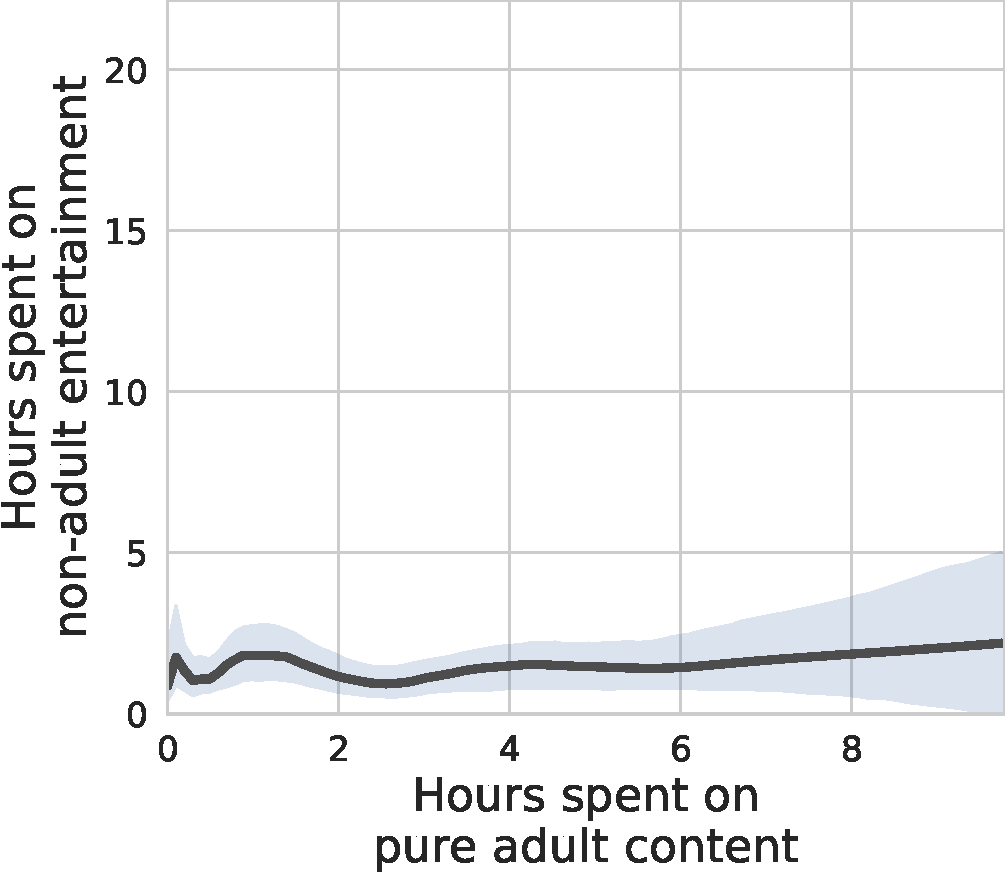
\includegraphics[width=\textwidth]{figs/tu_duration_entertainment-duration_pure_adult.pdf}
         \caption{Entertainment}
     \end{subfigure}
     \hfill
     \begin{subfigure}[b]{0.495\textwidth}
         \centering
         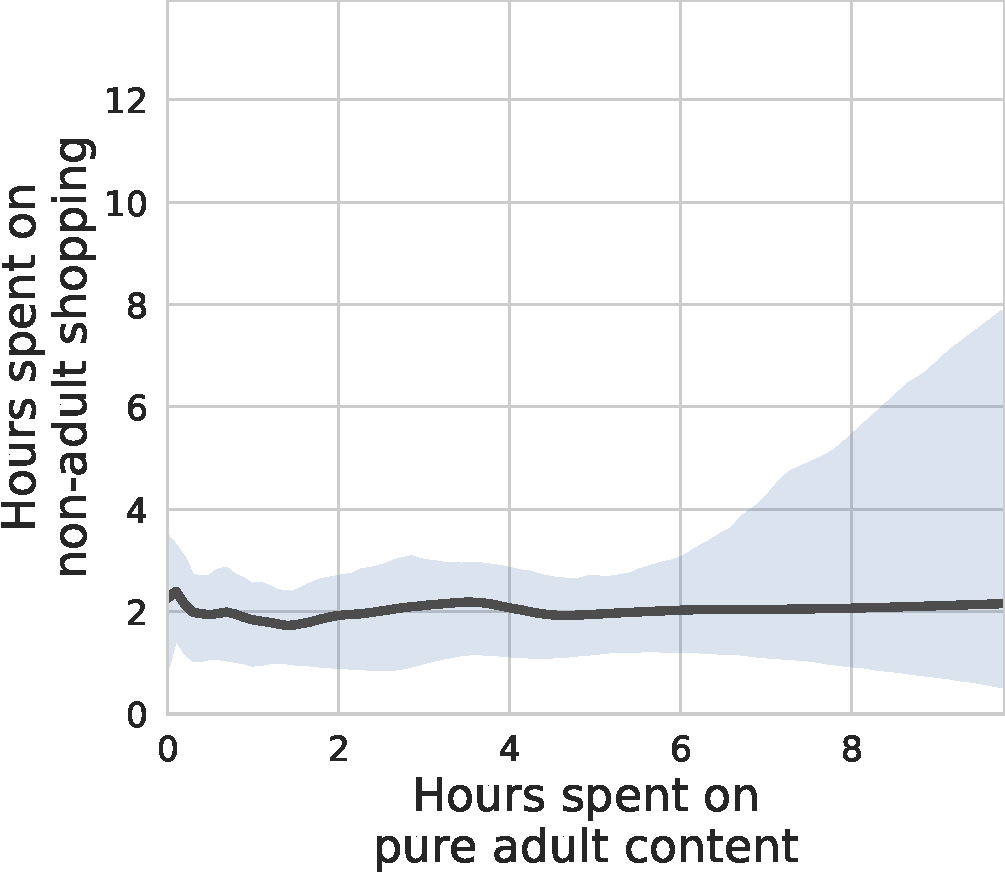
\includegraphics[width=\textwidth]{figs/tu_duration_shop-duration_pure_adult.pdf}
         \caption{Shopping}
     \end{subfigure}
\caption*{\footnotesize \emph{Notes:}
Lowess for time spent on online pornography (as defined in \nameref{subsec:measuring_porn_content}) vs time spent on other non-adult leisure (``entertainment'' and ``shopping'').
Observations above the 90th percentile are omitted. 
Non-adult entertainment sites are those with YouGov categories containing ``entertainment'' (e.g., ``Entertainment, Streaming Media'', ``Education, Entertainment, Streaming Media'', ``Business, Entertainment'', etc.)---top five of such sites are youtube.com, hideout.co, hulu.com, netflix.com, and yahoo.com.
Non-adult shopping sites are those with YouGov categories containing ``shopping'' (e.g., ``Shopping'', ``Business, Shopping'', ``Messageboards and Forums, Shopping'', etc.)---top five of such sites are amazon.com, ebay.com, walmart.com, etsy.com, capitaloneshopping.com, and craigslist.org.
Top five pure adult sites are: xvideos.com, pornhub.com, xnxx.com, rule34.xxx, and xhamster.com (see \cref{fig:top25_adult}).
Each estimation in the Lowess uses .3 of the sample data.
The 95\% confidence intervals shaded in blue are bootstrapped (n = 1000).
Swapping the horizontal axis for any adult content looks similar in \cref{fig:tu_prop_entertainment-prop_adult_duration}. 
}
\end{figure}


\clearpage
\setcounter{table}{0}
\setcounter{figure}{0}
\setcounter{equation}{0}
% =============================================================================
\FloatBarrier
\renewcommand{\thetable}{D\arabic{table}}
\renewcommand{\thefigure}{D\arabic{figure}}
\renewcommand{\theequation}{D\arabic{equation}}
\subsection{D. \smDTitle{}}\label{sm:smD}
% =============================================================================

First, we evaluate the density of the timing of visits to online pornography sites using 24-hour bins. As anticipated, most visits to online pornography sites occur around midnight. We also observe considerable traffic around the midday (1--3 pm, \cref{fig:time-of-day-consumption}). Both these observations track with \cite{webporn}'s findings using web session data. Second, we repeat the evaluation of the density of the timing of visits but split by partisanship.

The densities suggest that Democratic traffic to pornography sites is concentrated around midnight (11 pm--1 am) while the Republican traffic is concentrated in the early morning (6 am--7 am, \cref{fig:time-of-day-consumption-by-party}).

Third, to formally test whether there are differences in time of consumption by partisanship, we begin by dividing traffic to online pornography sites into six 4-hour bins: (a) 4 am--8 am, (b) 8 am--12 pm, (c) 12 pm--4 pm, (d) 4 pm--8 pm, (e) 8 pm--12 am, and (f) 12 am--4 am. We code a visit depending on which time interval it occurred and regress that time-of-day window on partisanship, weighted by the dwelling time of the visit. Cognizant of the somewhat ad-hoc splits for the time-of-day windows and that we are creating multiple outcome variables, we subject p-values of the partisan point estimate to Bonferroni correction in addition to the adjustments for individual-level demographics.

\begin{figure}[ht]
\centering
\caption{Time-of-Day Traffic to Online Pornography Sites}
    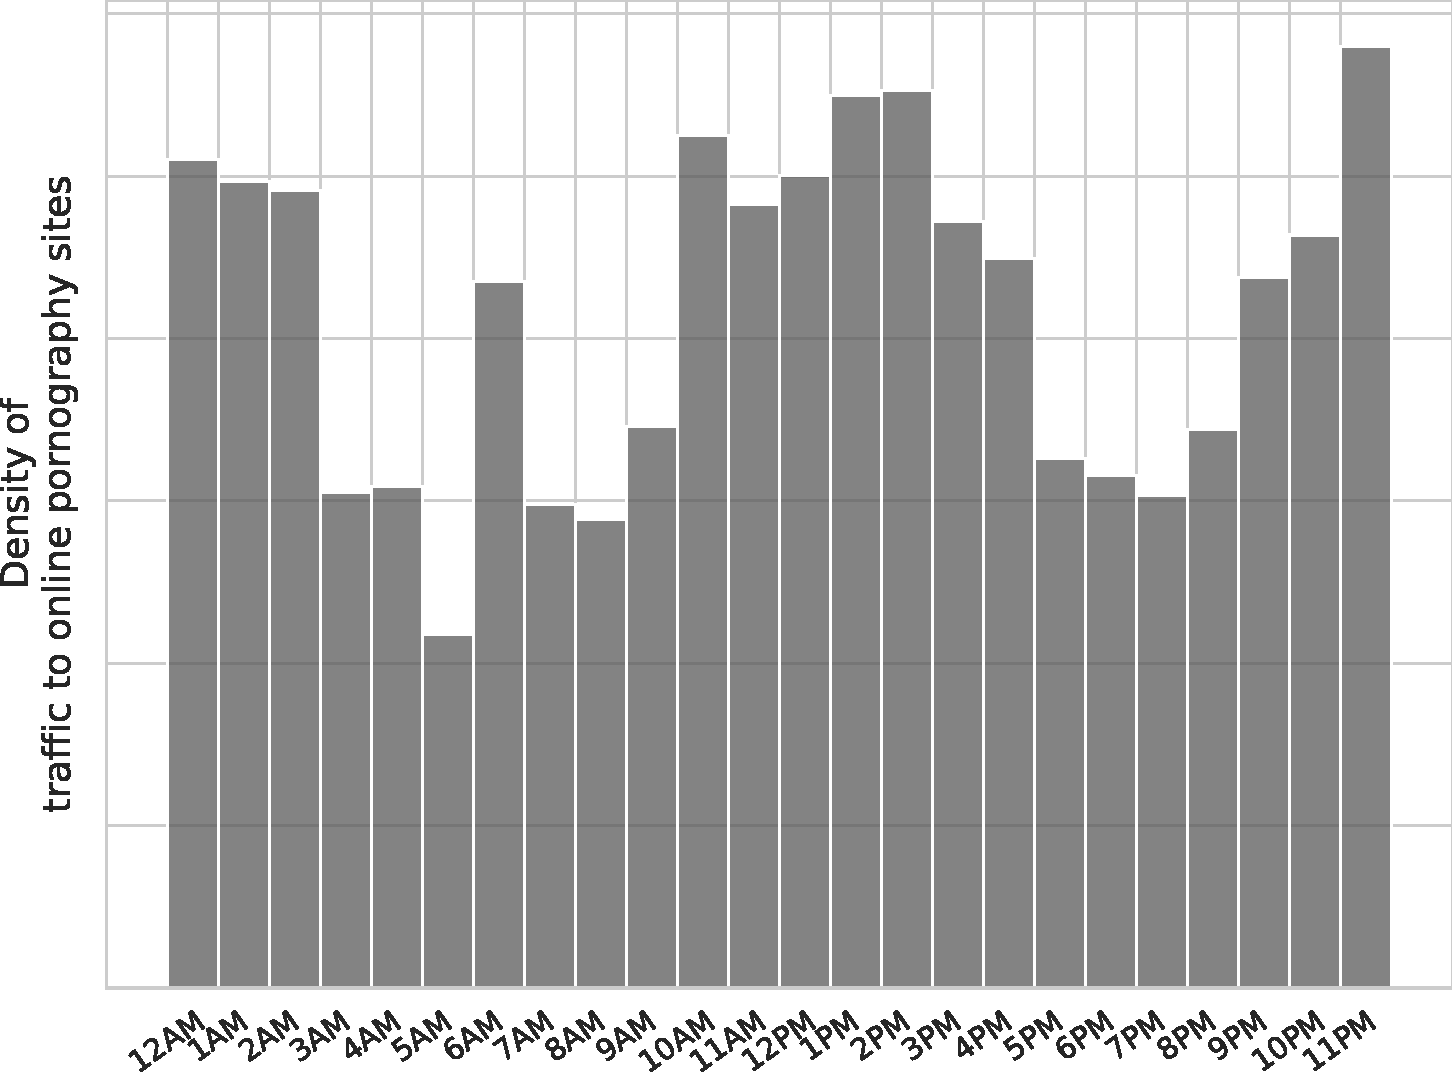
\includegraphics[width=.75\linewidth]{figs/time-of-day-consumption.pdf}
\caption*{\footnotesize \emph{Notes:} 
        Density plot of traffic to online pornography sites.
        Data is at the individual-browsing level with timestamped visits to pornography sites (individual-browsing n = 84,289).
        Each of the 24 bins corresponds to an hour of the day.
	}
    \label{fig:time-of-day-consumption}
\end{figure}

\begin{figure}[ht]
\centering
\caption{Time-of-Day Traffic to Online Pornography Sites by Party}
    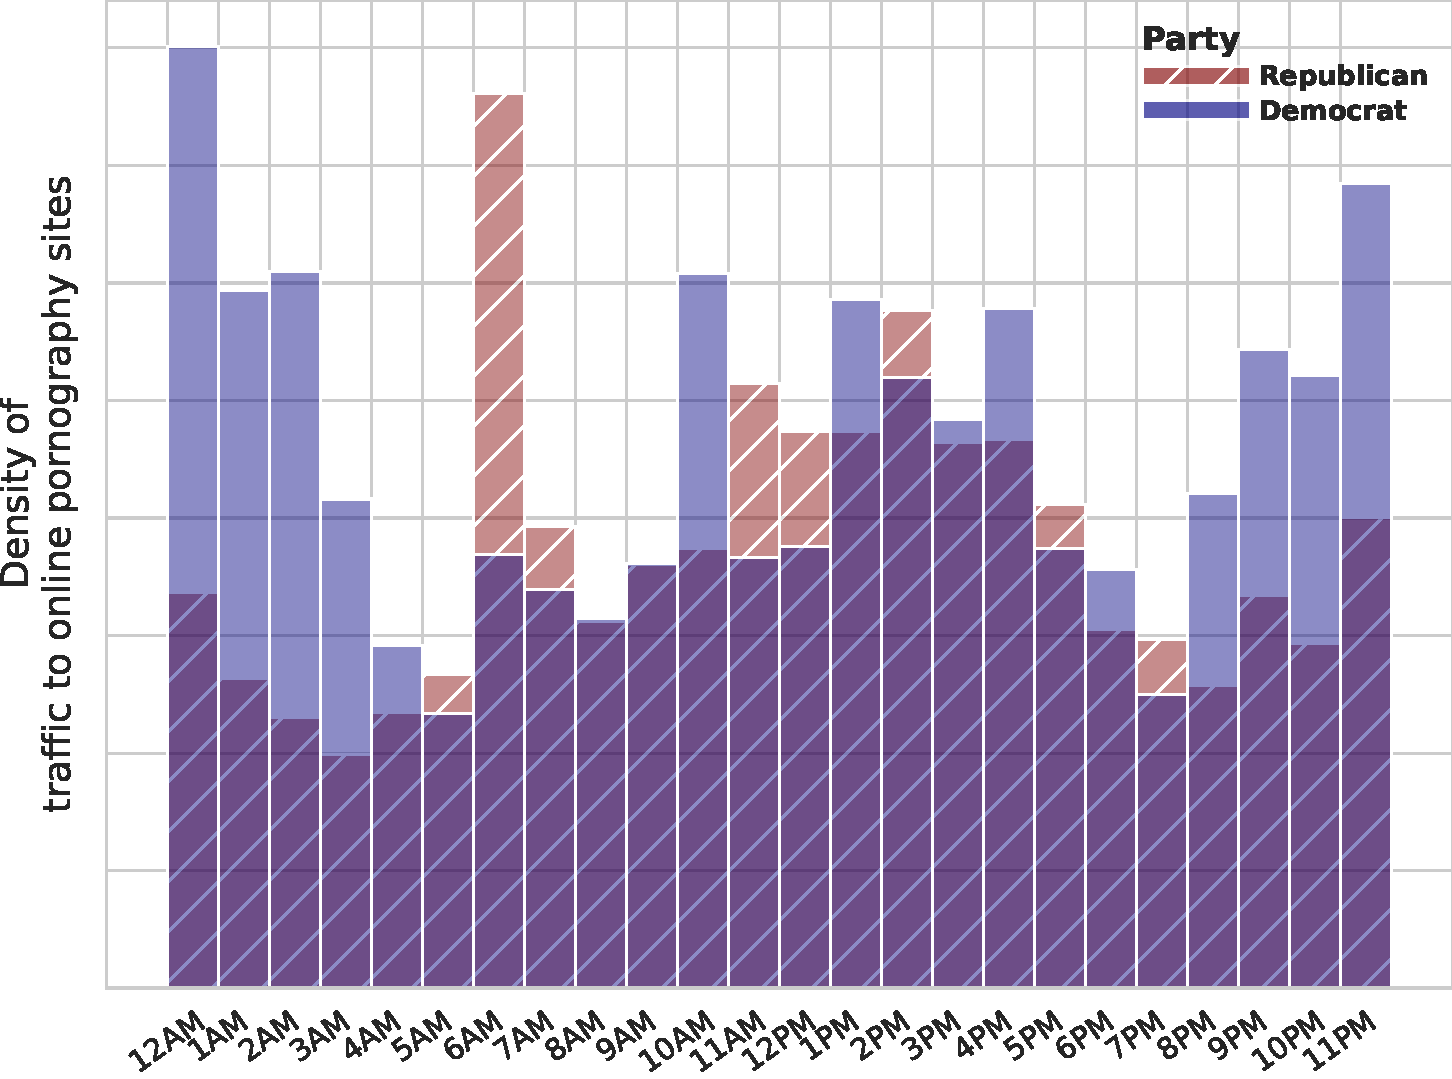
\includegraphics[width=.75\linewidth]{figs/time-of-day-consumption-by-party.pdf}
\caption*{\footnotesize \emph{Notes:} 
        Density plot of traffic to online pornography sites by partisanship (indicated by colors); bars for Republican consumption are also hatched.
        Data is at the individual-browsing level with timestamped visits to pornography sites (individual-browsing n = 59,324).
        Each of the 24 bins corresponds to an hour of the day.
        See \cref{tab:regtab_wls_visit_timing_4hrbins}, which reports formal tests of differences in time-of-day visits by party.
	}
    \label{fig:time-of-day-consumption-by-party}
\end{figure}

\begin{figure}[!ht]
\centering
\caption{Time-of-Day Traffic to Online Pornography Sites by Party}
    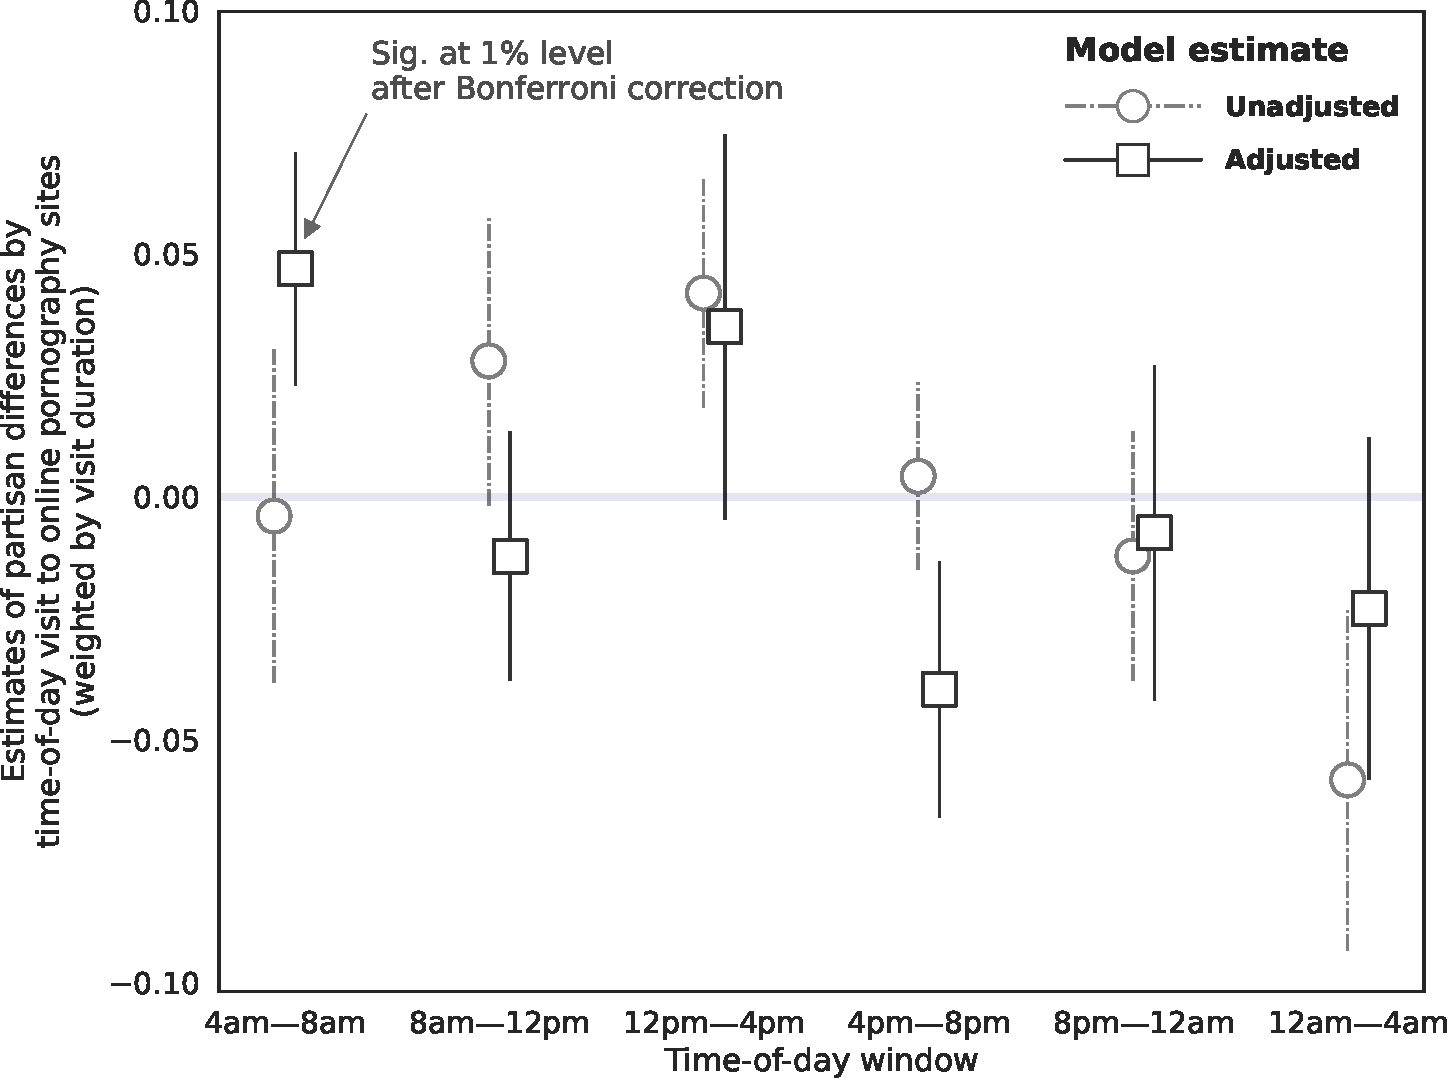
\includegraphics[width=.85\linewidth]{figs/time-of-day-wls-estimates.pdf}
\caption*{\footnotesize \emph{Notes:} 
        Estimates of partisan differences in time-of-day visits to online pornography sites.
        Points represent differences between Republicans relative to Democrats (reference category)---interpreted as proportion differences.
        The adjusted estimate, which is significant at the 1\% level after Bonferroni correction (at 4 am--8 am), is indicated in the figure.
        Vertical lines are 95\% confidence intervals.
        This figure offers an alternative visualization of \cref{tab:regtab_wls_visit_timing_4hrbins}.
	}
    \label{fig:time-of-day-wls-estimates}
\end{figure}

\cref{fig:time-of-day-wls-estimates} reports a summary of this exercise (\cref{tab:regtab_wls_visit_timing_4hrbins} reports the full set of estimates). The unadjusted estimates suggest that Republicans are more likely to consume pornography during midday (the 12 pm--4 pm window), relative to Democrats, which is significant at the 1 percent level after correction. Conversely, Republicans are less likely to consume pornography late at night (12 am--4 am). These unadjusted findings correspond somewhat to our evaluation of densities of visits by partisanship where Democrat visits to online pornography are concentrated around midnight (\cref{fig:time-of-day-consumption-by-party}).

Once we adjust for the individual-level demographics and for day-of-week fixed effects, Republicans are no longer more (or less) likely to consume pornography during the midday (or late at night). However, the adjusted estimates suggest that Republicans are more likely to consume pornography in the early morning (4 am--8 am), specifically five percentage points more likely, which is significant at the 1 percent level even after Bonferroni correction (indicated in \cref{fig:time-of-day-wls-estimates}).


\begin{table}[!ht] \centering \scriptsize \setlength\tabcolsep{9 pt} \setlength{\defaultaddspace}{0pt}
\def\sym#1{\ifmmode^{#1}\else\(^{#1}\)\fi}
\caption{Time-of-Day Traffic to Pornographic by Party}
\label{tab:regtab_wls_visit_timing_4hrbins}
\begin{adjustbox}{max width=\textwidth}
        \begin{tabular}{@{\hspace{0\tabcolsep}}l*{6}{D{.}{.}{-1}}@{\hspace{0\tabcolsep}}}
        \toprule\toprule
        &\multicolumn{1}{c}{(1)}         &\multicolumn{1}{c}{(2)}         &\multicolumn{1}{c}{(3)}         &\multicolumn{1}{c}{(4)}         &\multicolumn{1}{c}{(5)}         &\multicolumn{1}{c}{(6)}\\
        \cmidrule(l){2-7}
        &\multicolumn{6}{c}{\textbf{Panel A. WLS estimates}}\\
        &\multicolumn{6}{c}{Outcome variable is a binary variable based on time-of-day visit:}\\
        &\multicolumn{1}{c}{4am--8am}&\multicolumn{1}{c}{8am--12pm}&\multicolumn{1}{c}{12pm--4pm}&\multicolumn{1}{c}{4pm--8pm}&\multicolumn{1}{c}{8pm--12am}&\multicolumn{1}{c}{12am--4am}\\
        \cmidrule(l){2-7}
         Republican & -0.004 & 0.028 & 0.042\sym{\dagger} & 0.004 & -0.012 & -0.058\sym{\dagger} \\
& (0.017) & (0.015) & (0.012) & (0.010) & (0.013) & (0.018) \\
 Constant & 0.173\sym{\dagger} & 0.145\sym{\dagger} & 0.154\sym{\dagger} & 0.129\sym{\dagger} & 0.173\sym{\dagger} & 0.227\sym{\dagger} \\
& (0.013) & (0.009) & (0.008) & (0.006) & (0.008) & (0.010) \\
        \cmidrule(l){2-7}
        &\multicolumn{6}{c}{\textbf{Panel B. Adjusted WLS estimates}}\\
        &\multicolumn{6}{c}{Outcome variable is a binary variable based on time-of-day visit:}\\
        &\multicolumn{1}{c}{4am--8am}&\multicolumn{1}{c}{8am--12pm}&\multicolumn{1}{c}{12pm--4pm}&\multicolumn{1}{c}{4pm--8pm}&\multicolumn{1}{c}{8pm--12am}&\multicolumn{1}{c}{12am--4am}\\
        \cmidrule(l){2-7}
         Republican & 0.047\sym{\dagger} & -0.012 & 0.035 & -0.040\sym{**} & -0.007 & -0.023 \\
& (0.012) & (0.013) & (0.020) & (0.013) & (0.018) & (0.018) \\
 Female & 0.233\sym{\dagger} & 0.019 & -0.086\sym{\dagger} & -0.077\sym{\dagger} & -0.058\sym{**} & -0.031 \\
& (0.025) & (0.019) & (0.023) & (0.013) & (0.020) & (0.020) \\
 Educ (HS) & 0.064 & 0.045 & 0.040\sym{*} & 0.032 & -0.118\sym{\dagger} & -0.062 \\
& (0.033) & (0.036) & (0.017) & (0.018) & (0.032) & (0.045) \\
 Educ (some coll.) & -0.025 & 0.027 & 0.158\sym{\dagger} & 0.035\sym{*} & -0.095\sym{**} & -0.101\sym{*} \\
& (0.030) & (0.037) & (0.018) & (0.017) & (0.033) & (0.044) \\
 Educ (coll. grad.) & -0.007 & -0.019 & 0.121\sym{\dagger} & 0.040\sym{*} & -0.041 & -0.093\sym{*} \\
& (0.031) & (0.035) & (0.018) & (0.018) & (0.032) & (0.042) \\
 Age & 0.006\sym{*} & 0.011\sym{\dagger} & -0.007\sym{**} & -0.001 & -0.008\sym{\dagger} & -0.001 \\
& (0.002) & (0.003) & (0.002) & (0.002) & (0.002) & (0.003) \\
 Age$^2$ & -0.000 & -0.000\sym{\dagger} & 0.000\sym{\dagger} & 0.000 & 0.000\sym{*} & -0.000 \\
& (0.000) & (0.000) & (0.000) & (0.000) & (0.000) & (0.000) \\
 Race (Black) & 0.144\sym{\dagger} & -0.066\sym{\dagger} & -0.024 & -0.041\sym{**} & -0.071\sym{\dagger} & 0.058\sym{**} \\
& (0.019) & (0.014) & (0.020) & (0.016) & (0.019) & (0.022) \\
 Race (Hispanic) & 0.010 & -0.031 & 0.004 & -0.059\sym{\dagger} & 0.053\sym{*} & 0.022 \\
& (0.023) & (0.021) & (0.023) & (0.016) & (0.023) & (0.022) \\
 Race (Asian) & 0.101\sym{\dagger} & 0.065\sym{**} & -0.086\sym{\dagger} & -0.105\sym{\dagger} & -0.021 & 0.046 \\
& (0.029) & (0.024) & (0.024) & (0.015) & (0.025) & (0.028) \\
 Race (Other) & -0.002 & 0.037 & 0.030 & 0.069\sym{**} & -0.045\sym{*} & -0.089\sym{\dagger} \\
& (0.018) & (0.022) & (0.023) & (0.022) & (0.020) & (0.015) \\
 Region (MW) & -0.051\sym{**} & -0.040 & 0.066\sym{\dagger} & 0.053\sym{\dagger} & 0.113\sym{\dagger} & 0.059\sym{*} \\
& (0.019) & (0.023) & (0.016) & (0.016) & (0.022) & (0.027) \\
 Region (South) & 0.024 & -0.086\sym{\dagger} & 0.002 & 0.010 & 0.096\sym{\dagger} & 0.154\sym{\dagger} \\
& (0.014) & (0.013) & (0.013) & (0.011) & (0.013) & (0.017) \\
 Region (West) & 0.014 & -0.014 & 0.034\sym{*} & 0.052\sym{\dagger} & 0.057\sym{\dagger} & 0.057\sym{**} \\
& (0.016) & (0.015) & (0.015) & (0.011) & (0.014) & (0.019) \\
 Constant & -0.106\sym{*} & -0.130\sym{*} & 0.225\sym{\dagger} & 0.147\sym{\dagger} & 0.371\sym{\dagger} & 0.293\sym{\dagger} \\
& (0.053) & (0.058) & (0.038) & (0.034) & (0.050) & (0.071) \\
    \bottomrule
    \end{tabular}
    \end{adjustbox}
    \caption*{\scriptsize
    The table reports weighted least squares estimates from regressing a binary variable based on time-of-day visits to online pornography on the Republican dummy.
    The unit of observation is at the individual web browsing level for traffic to pornography sites (n = 59,324).
    Each column represents dummy variables for each of the six 4-hour windows.
    Weights are the duration of each visit.
    Models also adjust for day-of-week fixed effects (not reported to conserve space).
    See also \cref{fig:time-of-day-consumption-by-party}, which provides descriptive evidence that the density in time-of-day traffic is different by party.
    Significance levels (uncorrected): $^{*}$ 0.05 $^{**}$0.01.
    P-values are Bonferroni-corrected for six tests---the $^\dagger$ indicates significance at the p = 0.01 level after adjustment.    
    }
\end{table}

\setcounter{table}{0}
\setcounter{figure}{0}
\setcounter{equation}{0}
% =============================================================================
\FloatBarrier
\renewcommand{\thetable}{E\arabic{table}}
\renewcommand{\thefigure}{E\arabic{figure}}
\renewcommand{\theequation}{E\arabic{equation}}
\subsection{E. \smETitle{}}\label{sm:smE}
% =============================================================================
\subsubsection{Piedomains}
%============================
% Figure of top 25 adultsites
%============================
\begin{figure}[ht]
	\centering
	\caption{Top 25 Pornography Sites (Piedomains)}
	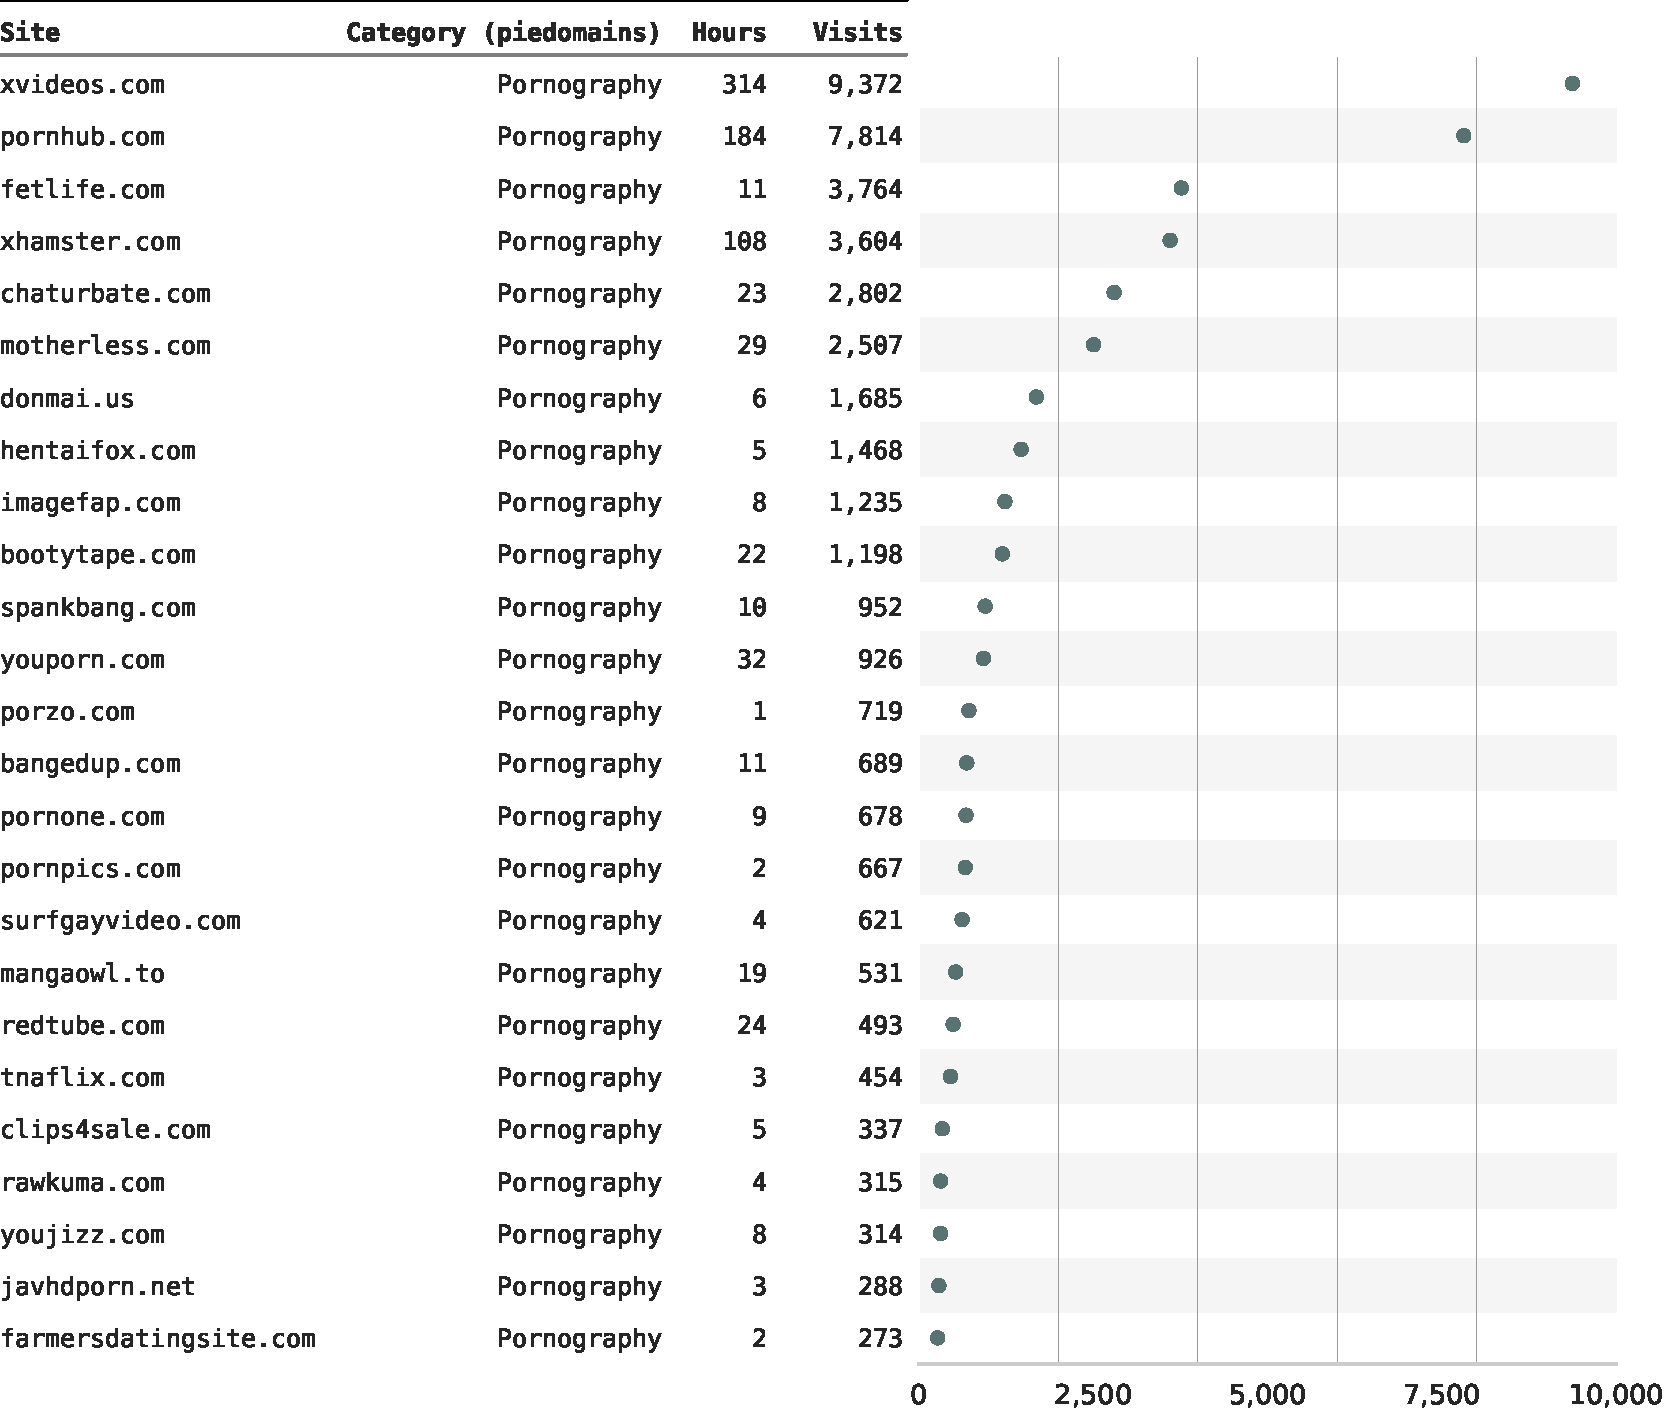
\includegraphics[width=\textwidth]{figs/top_25_adultsites_piedomains.pdf}
	\caption*{\footnotesize \emph{Notes:} 
		The table shows the top 25 pornographic sites that individuals visited in the sample period.
            All numbers are based on online visits during the one-month period.
		Pornography sites are categorized by Piedomains \citep{Chintalapati_piedomains_Predict_the_2022}.
            See \cref{fig:top25_adult} for a comparison with our base classification.
    	The \emph{Hours} column is the total number of hours that individuals in the sample spent on the site. 
    	The \emph{Visits} column is the total number of visits by individuals in the sample to the site.            
	}
	\label{fig:top25_adult_piedomains}
\end{figure}

\begin{figure}[ht]
	\centering
	\caption{Distribution of Partisan Differences in Hours Spent on Pornographic Sites (\texttt{piedomains})}
	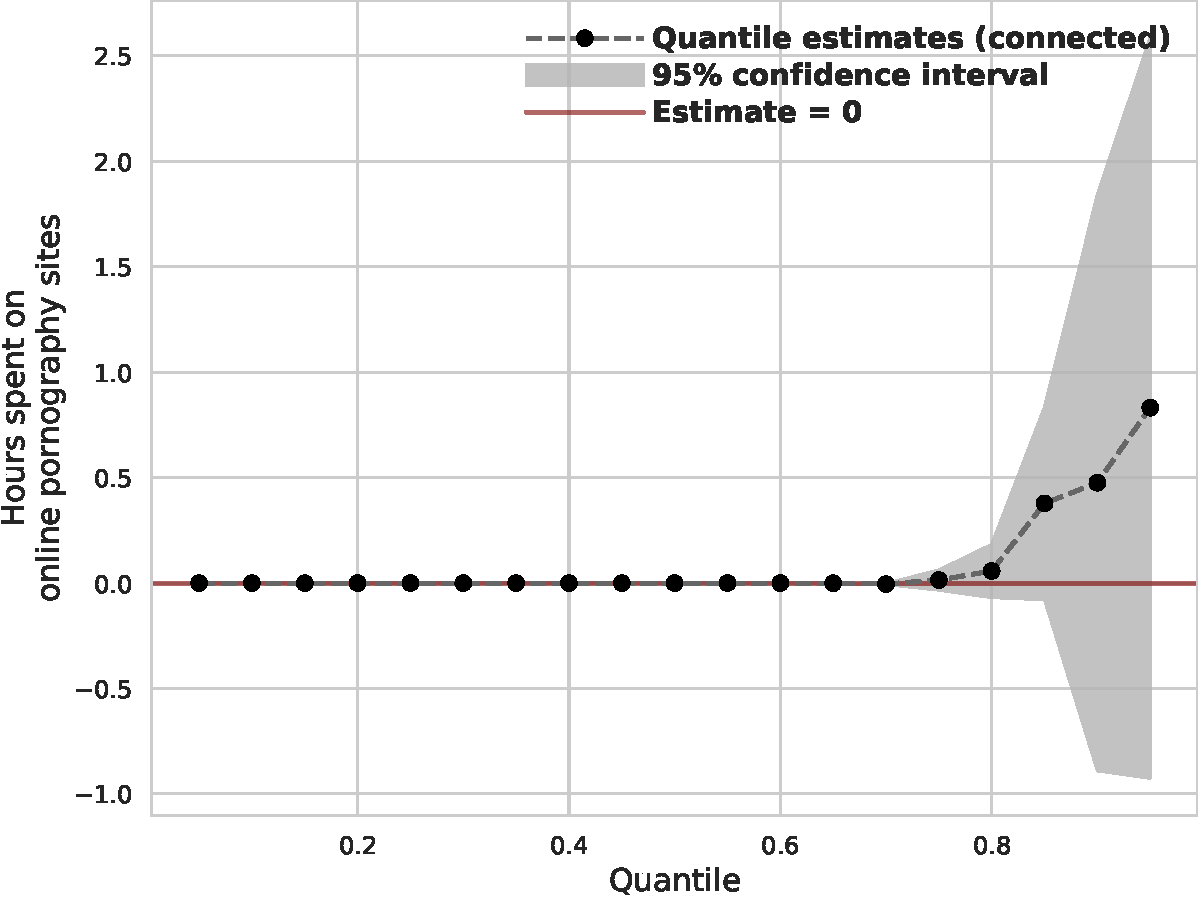
\includegraphics[width=.7\linewidth]{figs/piedomains_quantile_reg_duration_adult.pdf}
	\caption*{\footnotesize \emph{Notes:} 
		The dependent variable is the number of hours people spent on pornographic sites. Each point indicates the difference between Republicans and Democrats and corresponds to a quantile regression at the quantile indicated by the x-axis. 95\% confidence intervals constructed from standard errors. See \cref{fig:piedomains_quantile_regression_duration_covariates} for the same plot controlling for individual characteristics.
	}
	\label{fig:piedomains_quantile_regression_duration}
\end{figure}

%=====================================================
% Fig of quantile regression estimates
% Time Spent on Adult Sites by Party (with covariates) 
%=====================================================
\begin{figure}[ht]
	\centering
	\caption{Quantile Estimates--Hours Spent on Pornographic Sites by Party (with covariates, \texttt{piedomains})}
	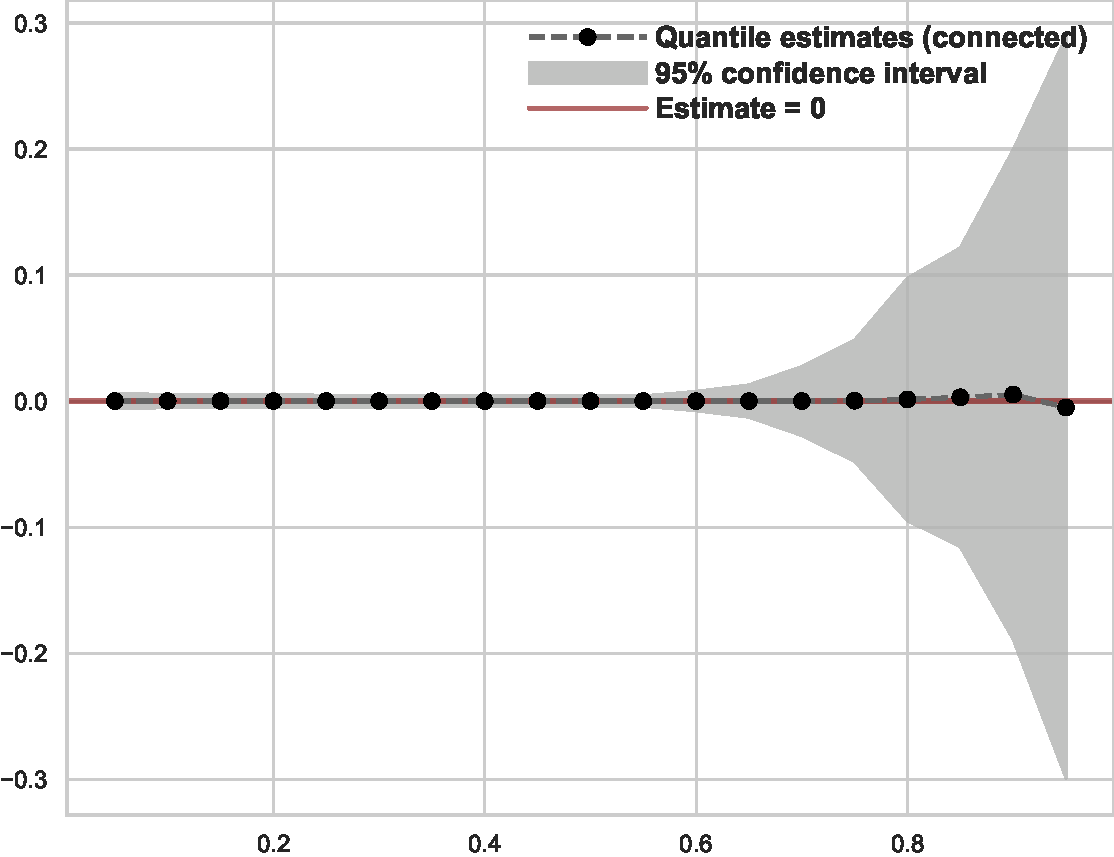
\includegraphics[width=.55\linewidth]{figs/quantile_reg_covariates_duration_adult.pdf}
	\caption*{\footnotesize \emph{Notes:} 
		The dependent variable is the number of hours individuals in our sample spent on pornographic sites.
		Each point indicates the difference between Republicans and Democrats and corresponds to a quantile regression at the quantile indicated by the x-axis.
		Covariates included gender (Female/Male), race (White/Black/Hispanic/Asian/Others), education level (no HS/HS graduate/some college/college graduate), age and its quadratic, and region (NE/MW/S/W).
		95\% confidence intervals constructed from standard errors.
		See \cref{fig:piedomains_quantile_regression_duration_covariates} for the same plot without covariates.
	}
	\label{fig:piedomains_quantile_regression_duration_covariates}
\end{figure}



\FloatBarrier
\clearpage
\subsubsection{Forcepoint ThreatSeeker}
%============================
% Figure of top 25 adultsites
%============================
\begin{figure}[!ht]
	\centering
	\caption{Top 25 Pornography Sites (Forcepoint ThreatSeeker)}
	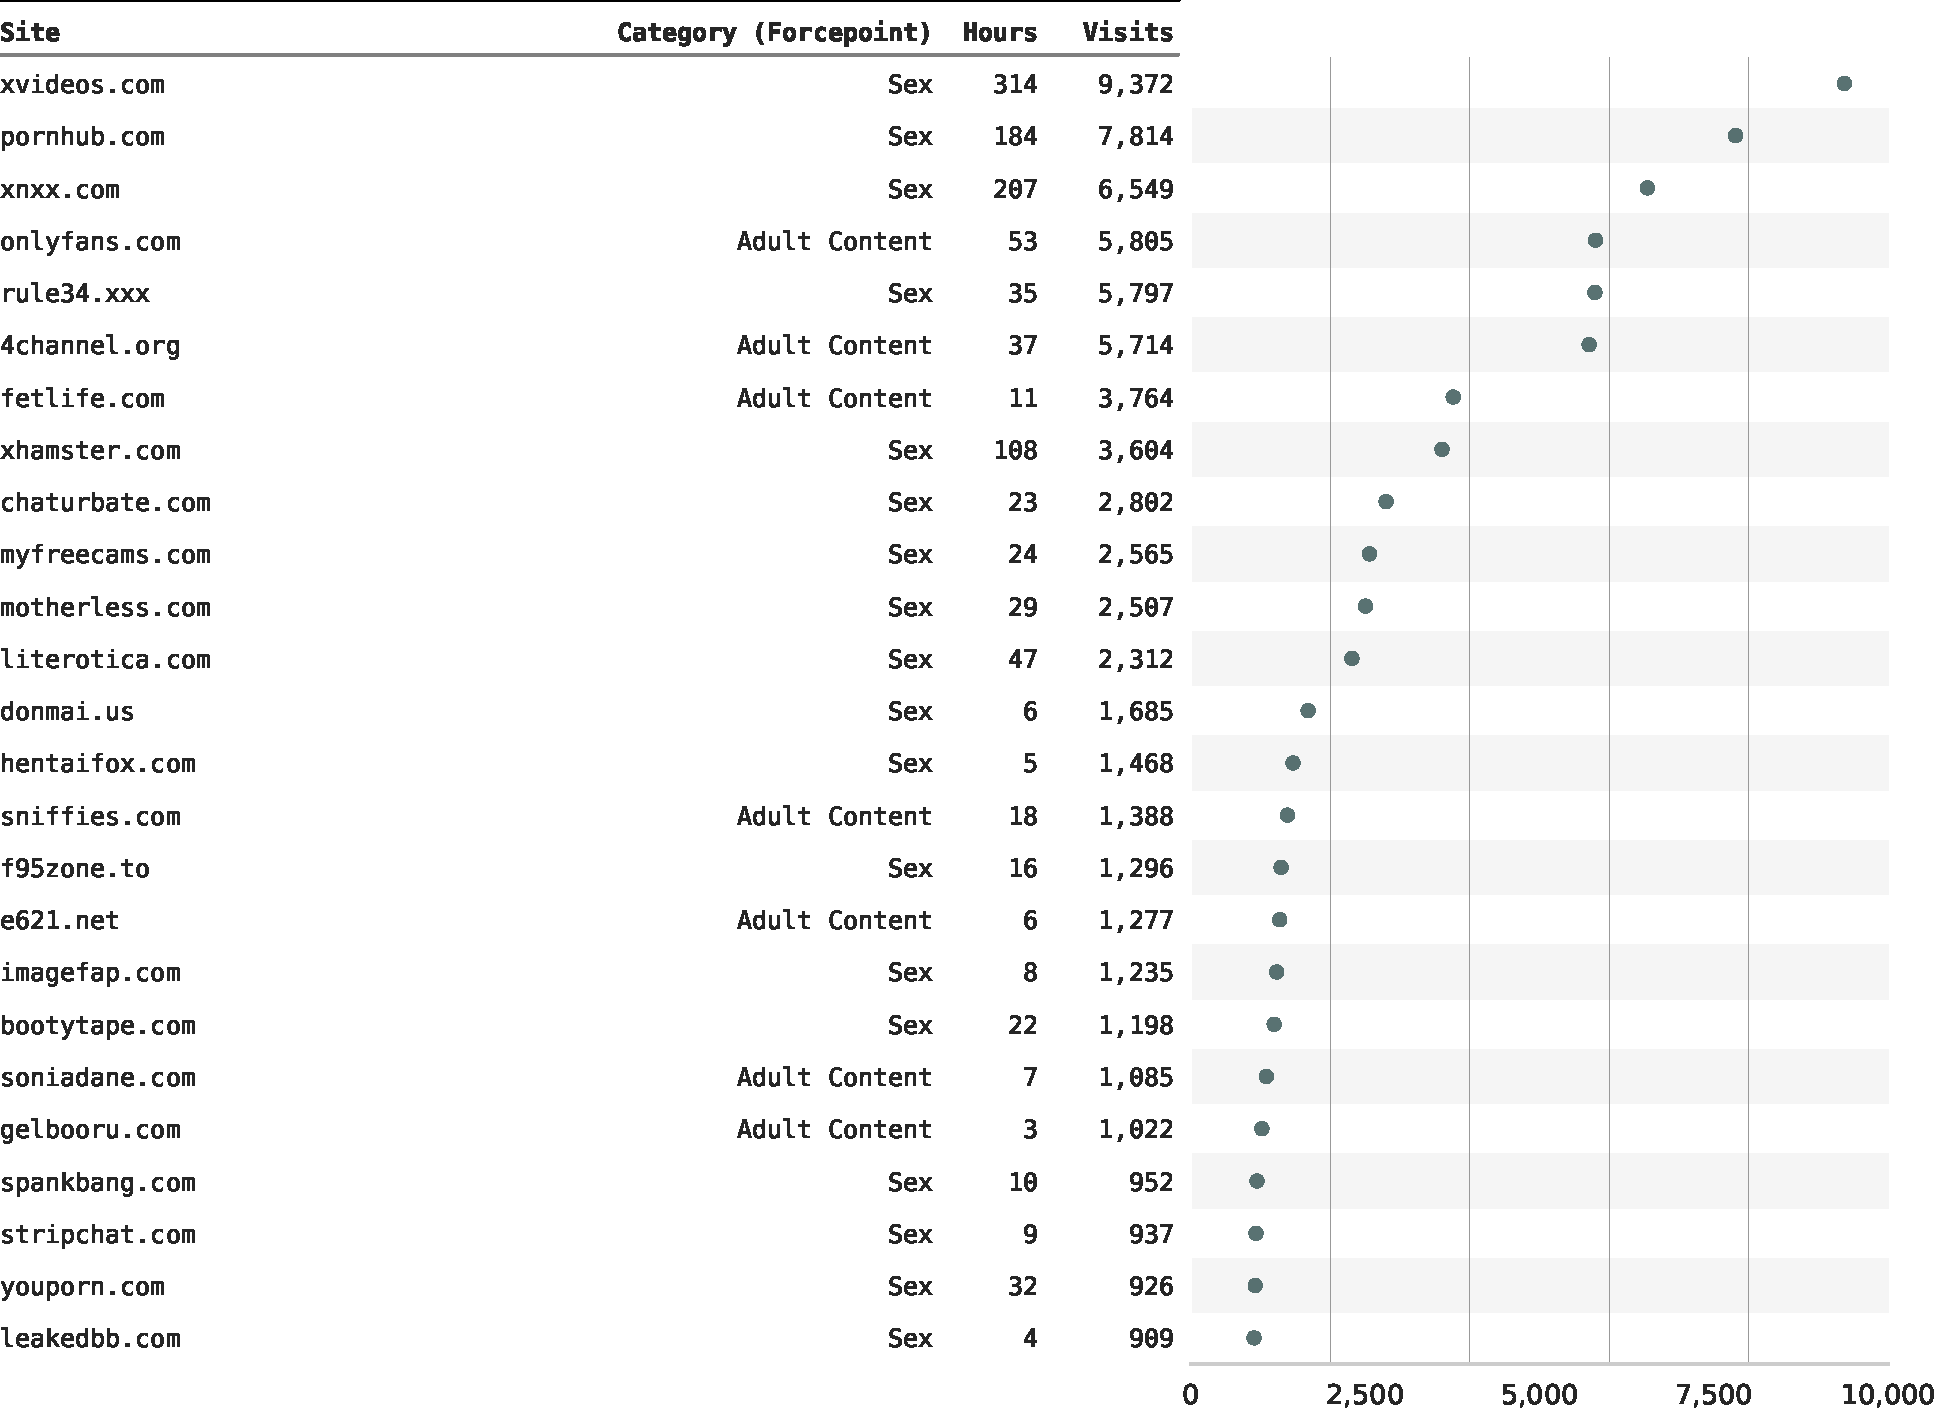
\includegraphics[width=\textwidth]{figs/top_25_adultsites_forcepoint_threatseeker.pdf}
	\caption*{\footnotesize \emph{Notes:} 
		The table shows the top 25 pornographic sites that individuals visited in the sample period.
            All numbers are based on online visits during the one-month period.
		Pornography sites are categorized by Forcepoint ThreatSeeker (``Sex'' or ``Adult Content'').
            See \cref{fig:top25_adult} for a comparison with our base classification.
    	The \emph{Hours} column is the total number of hours individuals in the sample spent on the site. 
    	The \emph{Visits} column is the total number of visits by individuals in the sample to the site.            
	}
	\label{fig:top25_adult_forcepoint}
\end{figure}


%===========================

% Quantile regressions

% Hours spent on adult sites

%===========================

\begin{figure}[t]
	\centering
	\caption{Distribution of Partisan Differences in Hours Spent on Pornographic Sites (Forcepoint ThreatSeeker)}
	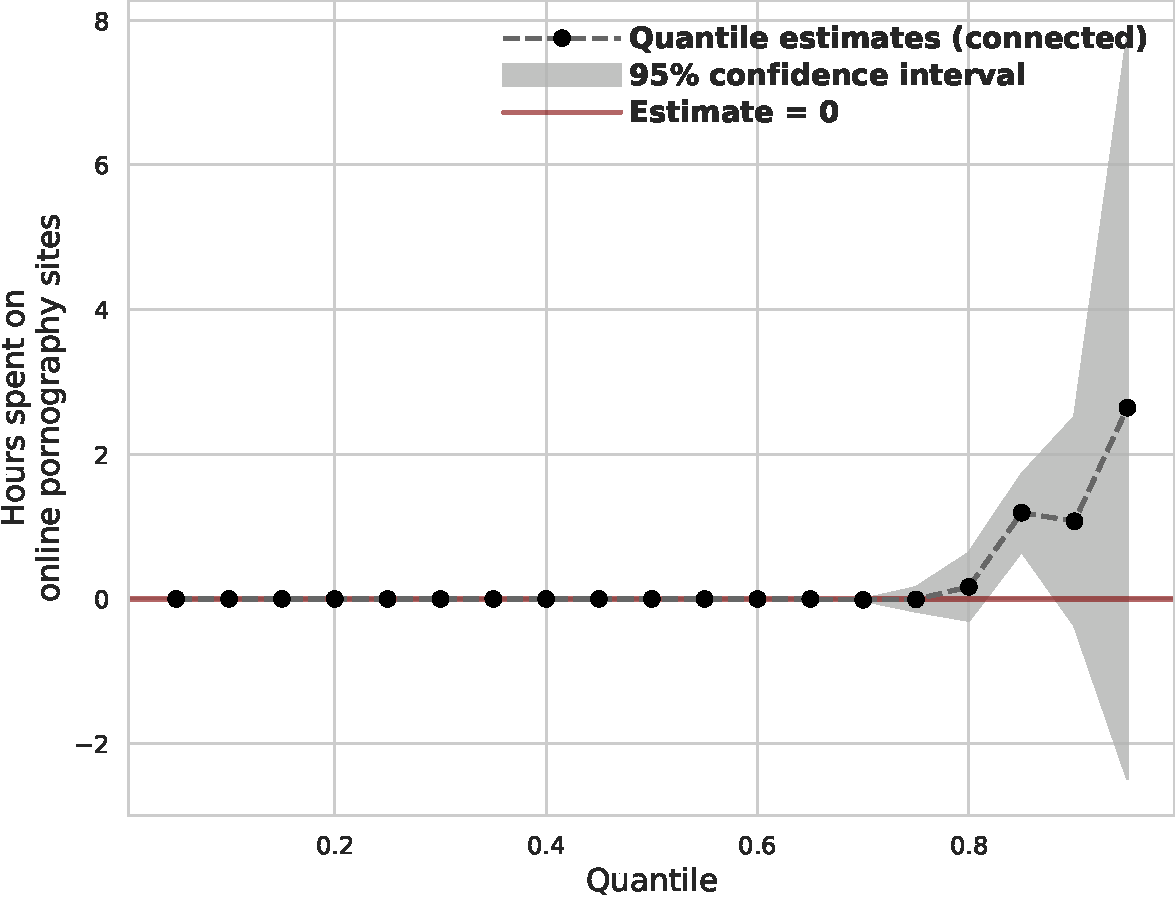
\includegraphics[width=.7\linewidth]{figs/forcepoint_quantile_reg_duration_adult.pdf}
	\caption*{\footnotesize \emph{Notes:} 
		The dependent variable is the number of hours individuals in our sample spent on pornographic sites.
		Each point indicates the difference between Republicans and Democrats and corresponds to a quantile regression at the quantile indicated by the x-axis.
		95\% confidence intervals constructed from standard errors.
		See \cref{fig:forcepoint_quantile_regression_duration_covariates} for the same plot controlling for individual characteristics.
	}
	\label{fig:forcepoint_quantile_regression_duration}
\end{figure}

%=====================================================
% Fig of quantile regression estimates
% Time Spent on Adult Sites by Party (with covariates) 
%=====================================================
\begin{figure}[ht]
	\centering
	\caption{Quantile Estimates--Hours Spent on Pornographic Sites by Party (with covariates, Forcepoint ThreatSeeker)}
	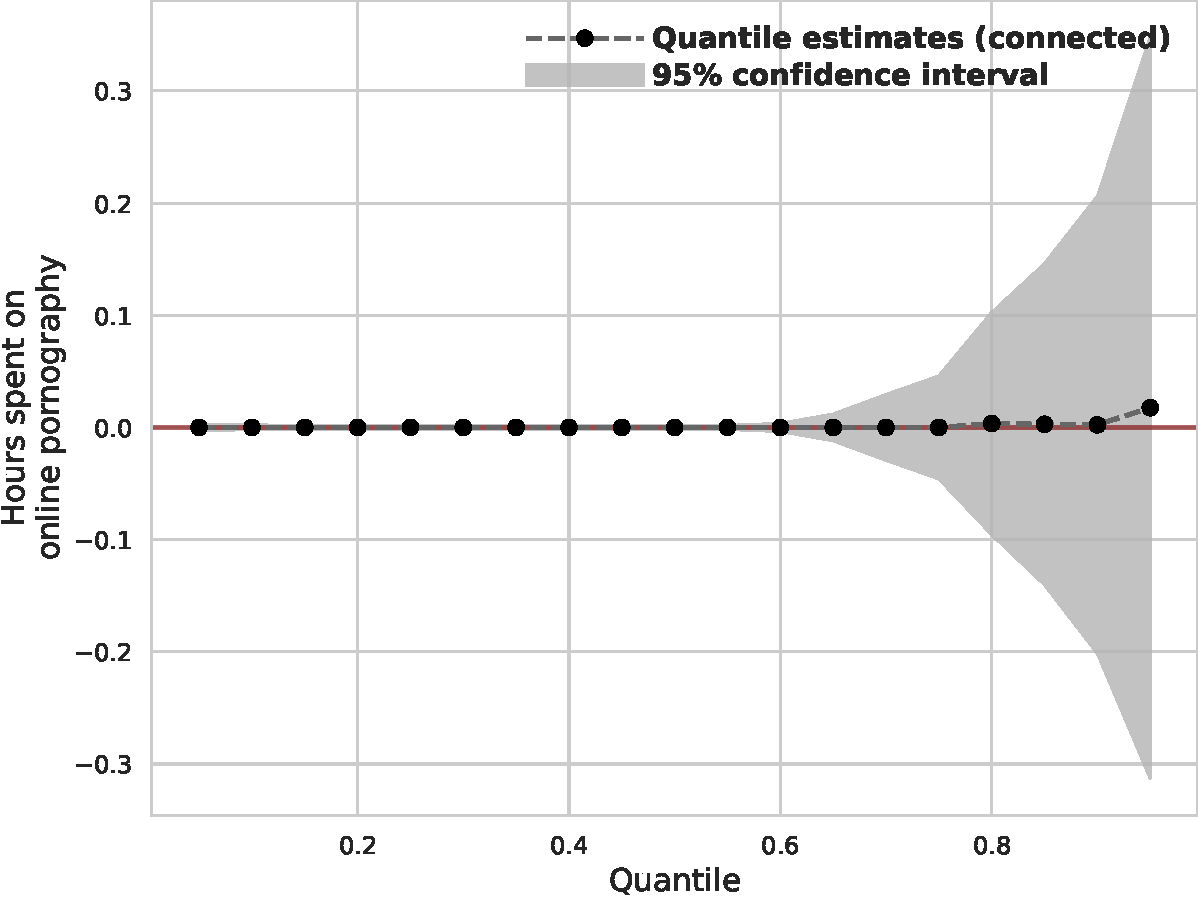
\includegraphics[width=.55\linewidth]{figs/forcepoint_quantile_reg_covariates_duration_adult.pdf}
	\caption*{\footnotesize \emph{Notes:} 
		The dependent variable is the number of hours individuals in our sample spent on pornographic sites.
		Each point indicates the difference between Republicans and Democrats and corresponds to a quantile regression at the quantile indicated by the x-axis.
		Covariates included on the right-hand side are gender (Female/Male), race (White/Black/Hispanic/Asian/Others), education level (no HS/HS graduate/some college/college graduate), age and its quadratic, and region (NE/MW/S/W).
		95\% confidence intervals constructed from standard errors.
		See \cref{fig:forcepoint_quantile_regression_duration_covariates} for the same plot without covariates.
	}
	\label{fig:forcepoint_quantile_regression_duration_covariates}
\end{figure}





\FloatBarrier
\clearpage
\subsubsection{Bitdefender}
%============================
% Figure of top 25 adultsites
%============================
\begin{figure}[ht]
	\centering
	\caption{Top 25 Pornography Sites (Bitdefender)}
	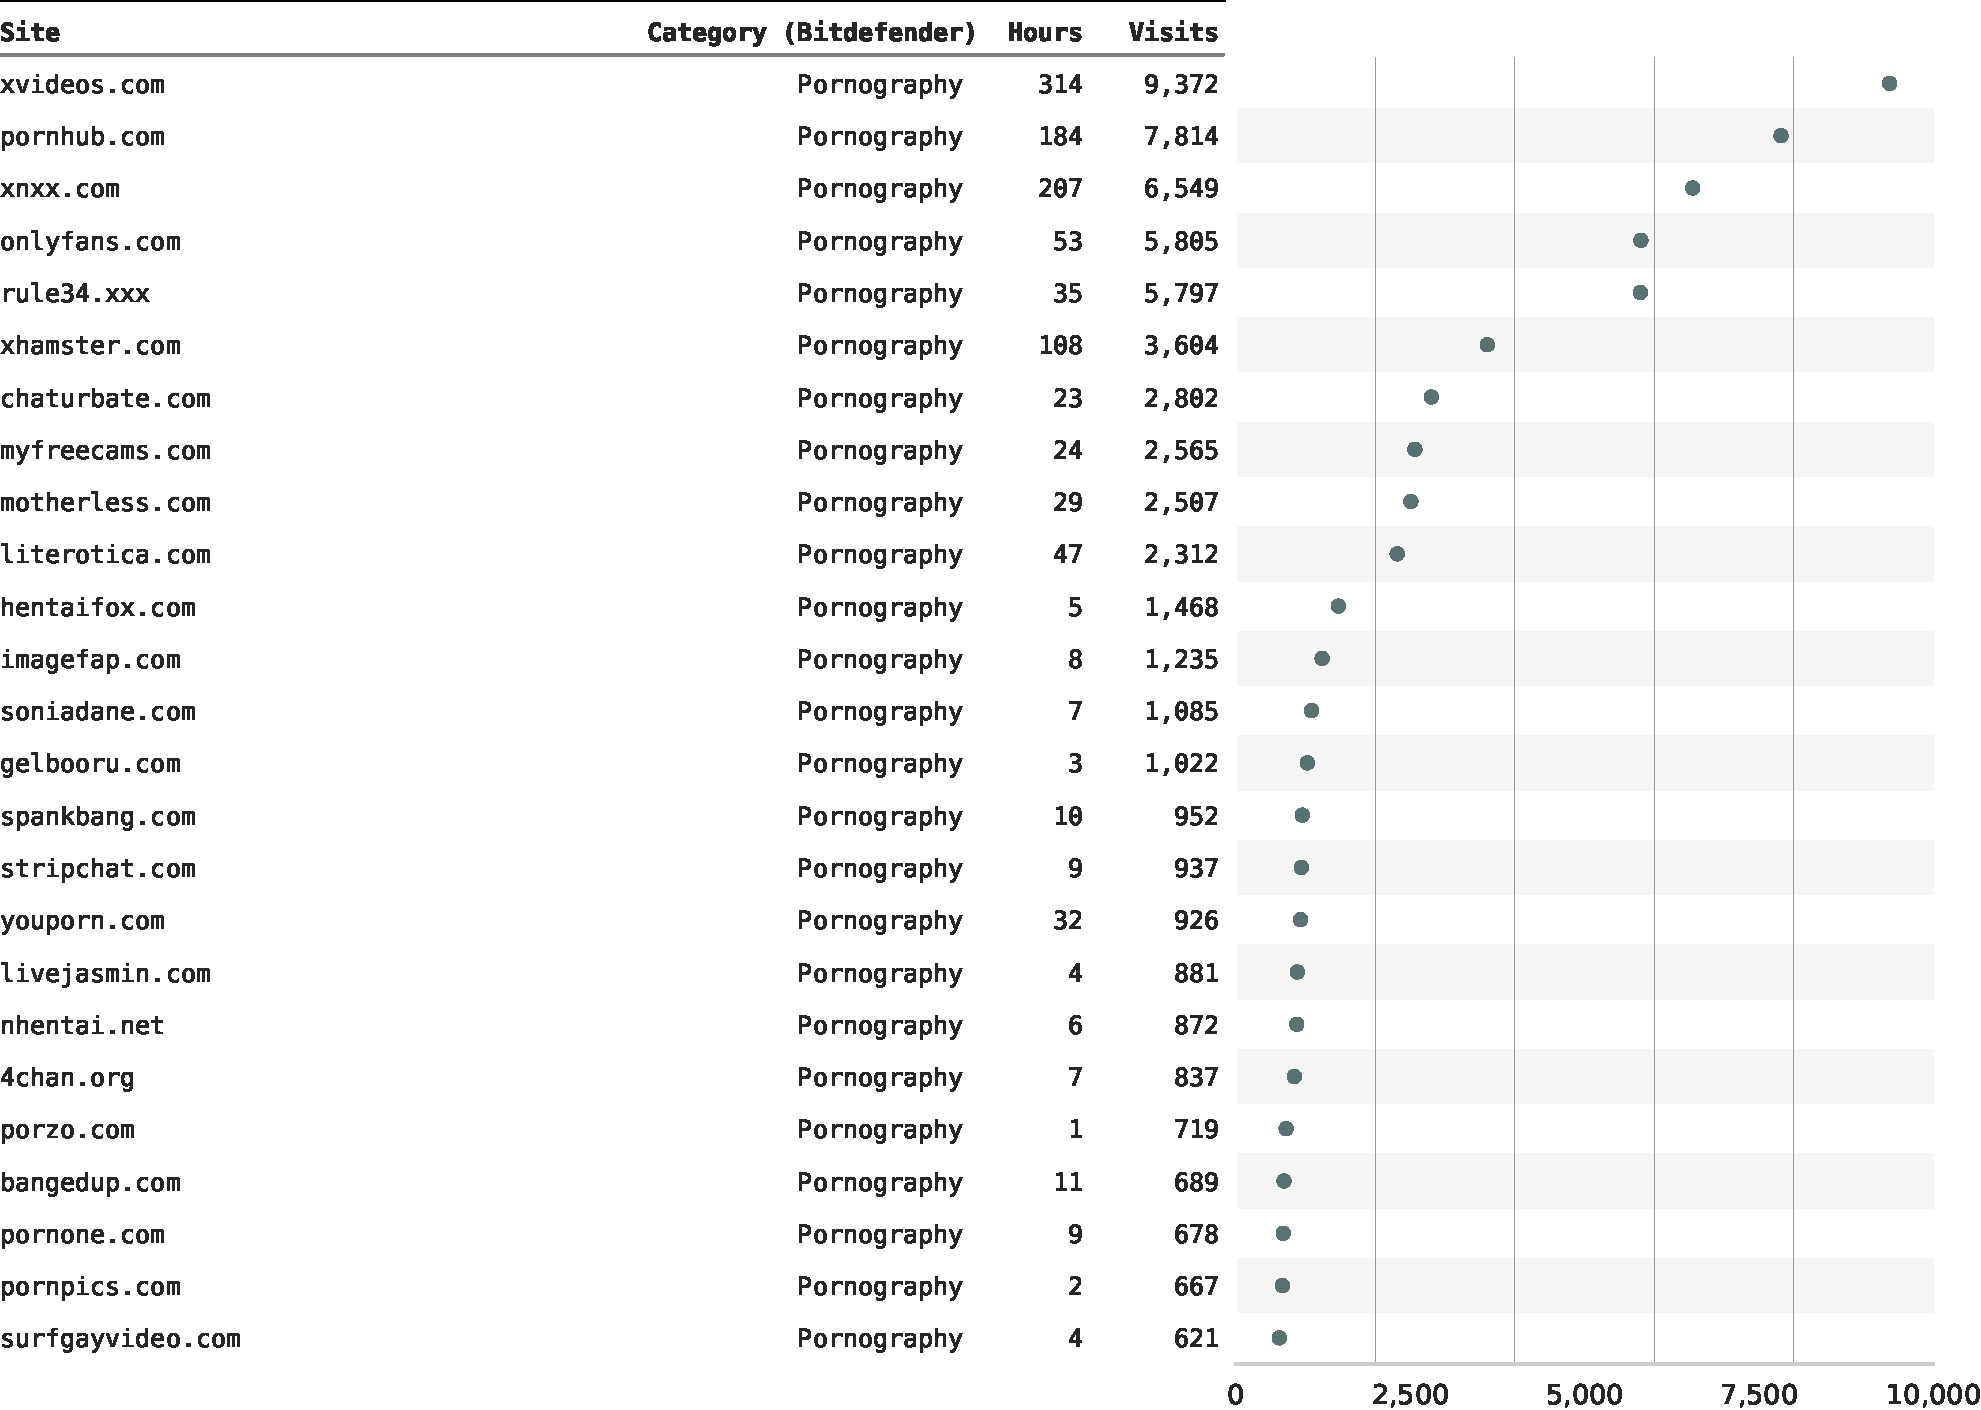
\includegraphics[width=\textwidth]{figs/top_25_adultsites_bitdefender.pdf}
	\caption*{\footnotesize \emph{Notes:} 
		The table shows the top 25 pornographic sites that individuals visited in the sample period.
            All numbers are based on online visits during the one-month period.
		Pornography sites are categorized by Bitdefender.
            See \cref{fig:top25_adult} for a comparison with our base classification.
    	The \emph{Hours} column is the total number of hours that individuals in the sample spent on the site. 
    	The \emph{Visits} column is the total number of visits by individuals in the sample to the site.            
	}
	\label{fig:top25_adult_bitdefender}
\end{figure}


%===========================

% Quantile regressions

% Hours spent on adult sites

%===========================

\begin{figure}[t]
	\centering
	\caption{Distribution of Partisan Differences in Hours Spent on Pornographic Sites (Bitdefender)}
	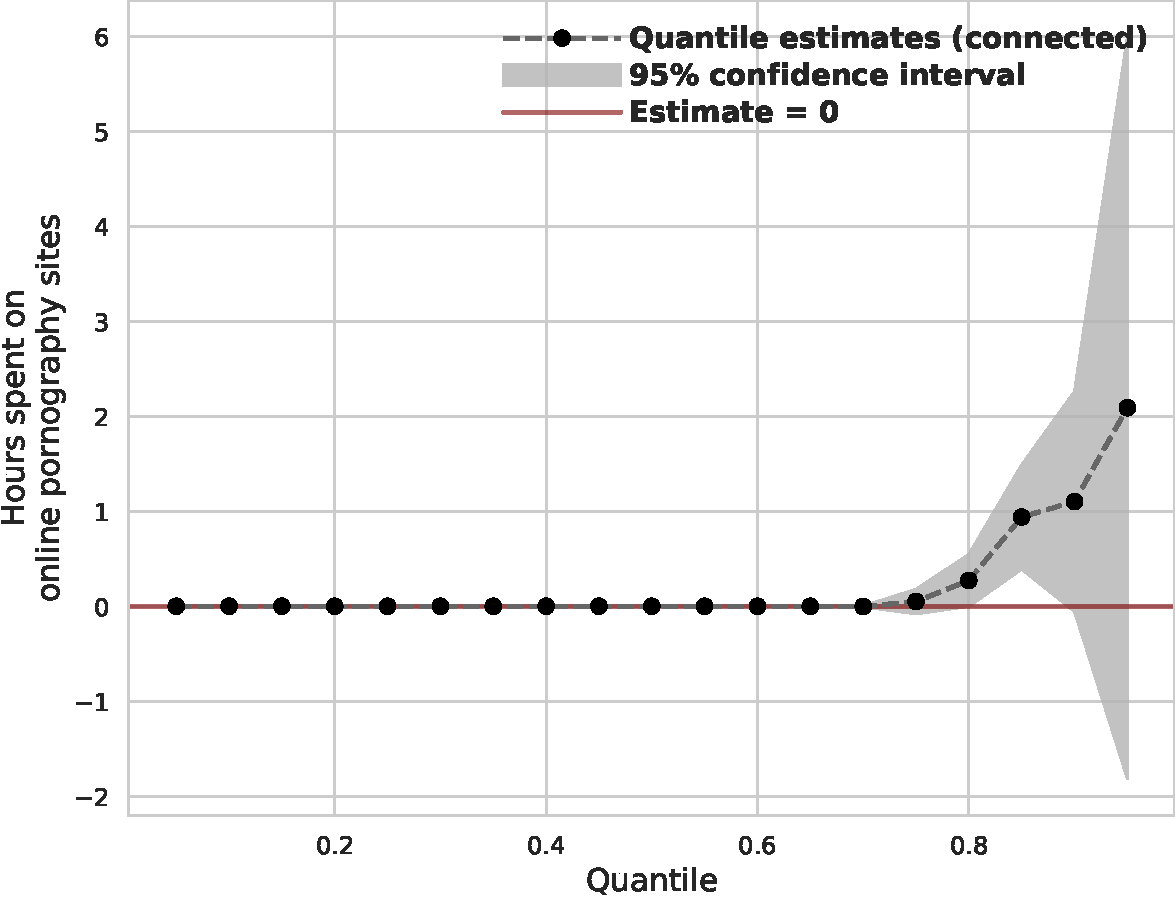
\includegraphics[width=.7\linewidth]{figs/bitdefender_quantile_reg_duration_adult.pdf}
	\caption*{\footnotesize \emph{Notes:} 
		The dependent variable is the number of hours individuals in our sample spent on pornographic sites.
		Each point indicates the difference between Republicans and Democrats and corresponds to a quantile regression at the quantile indicated by the x-axis.
		95\% confidence intervals constructed from standard errors.
		See \cref{fig:bitdefender_quantile_regression_duration_covariates} for the same plot controlling for individual characteristics.
	}
	\label{fig:bitdefender_quantile_regression_duration}
\end{figure}

%=====================================================
% Fig of quantile regression estimates
% Time Spent on Adult Sites by Party (with covariates) 
%=====================================================
\begin{figure}[ht]
	\centering
	\caption{Quantile Estimates--Hours Spent on Pornographic Sites by Party (with covariates, Bitdefender)}
	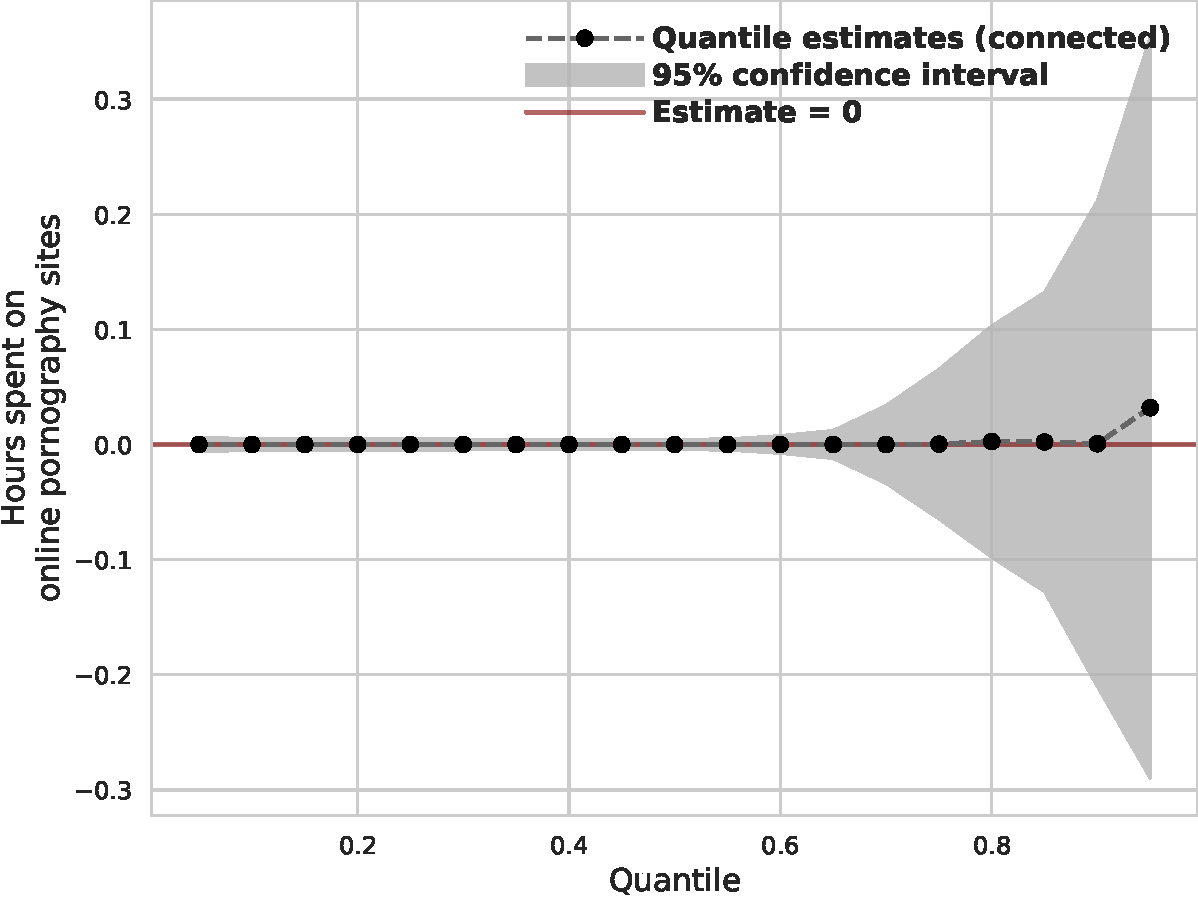
\includegraphics[width=.55\linewidth]{figs/bitdefender_quantile_reg_covariates_duration_adult.pdf}
	\caption*{\footnotesize \emph{Notes:} 
		The dependent variable is the number of hours individuals in our sample spent on pornographic sites.
		Each point indicates the difference between Republicans and Democrats and corresponds to a quantile regression at the quantile indicated by the x-axis.
		Covariates included gender (Female/Male), race (White/Black/Hispanic/Asian/Others), education level (no HS/HS graduate/some college/college graduate), age and its quadratic, and region (NE/MW/S/W).
		95\% confidence intervals constructed from standard errors.
		See \cref{fig:bitdefender_quantile_regression_duration_covariates} for the same plot without covariates.
	}
	\label{fig:bitdefender_quantile_regression_duration_covariates}
\end{figure}


\FloatBarrier
\clearpage
\subsubsection{alphaMountain}
%============================
% Figure of top 25 adultsites
%============================
\begin{figure}[!ht]
	\centering
	\caption{Top 25 Pornography Sites (alphaMountain)}
	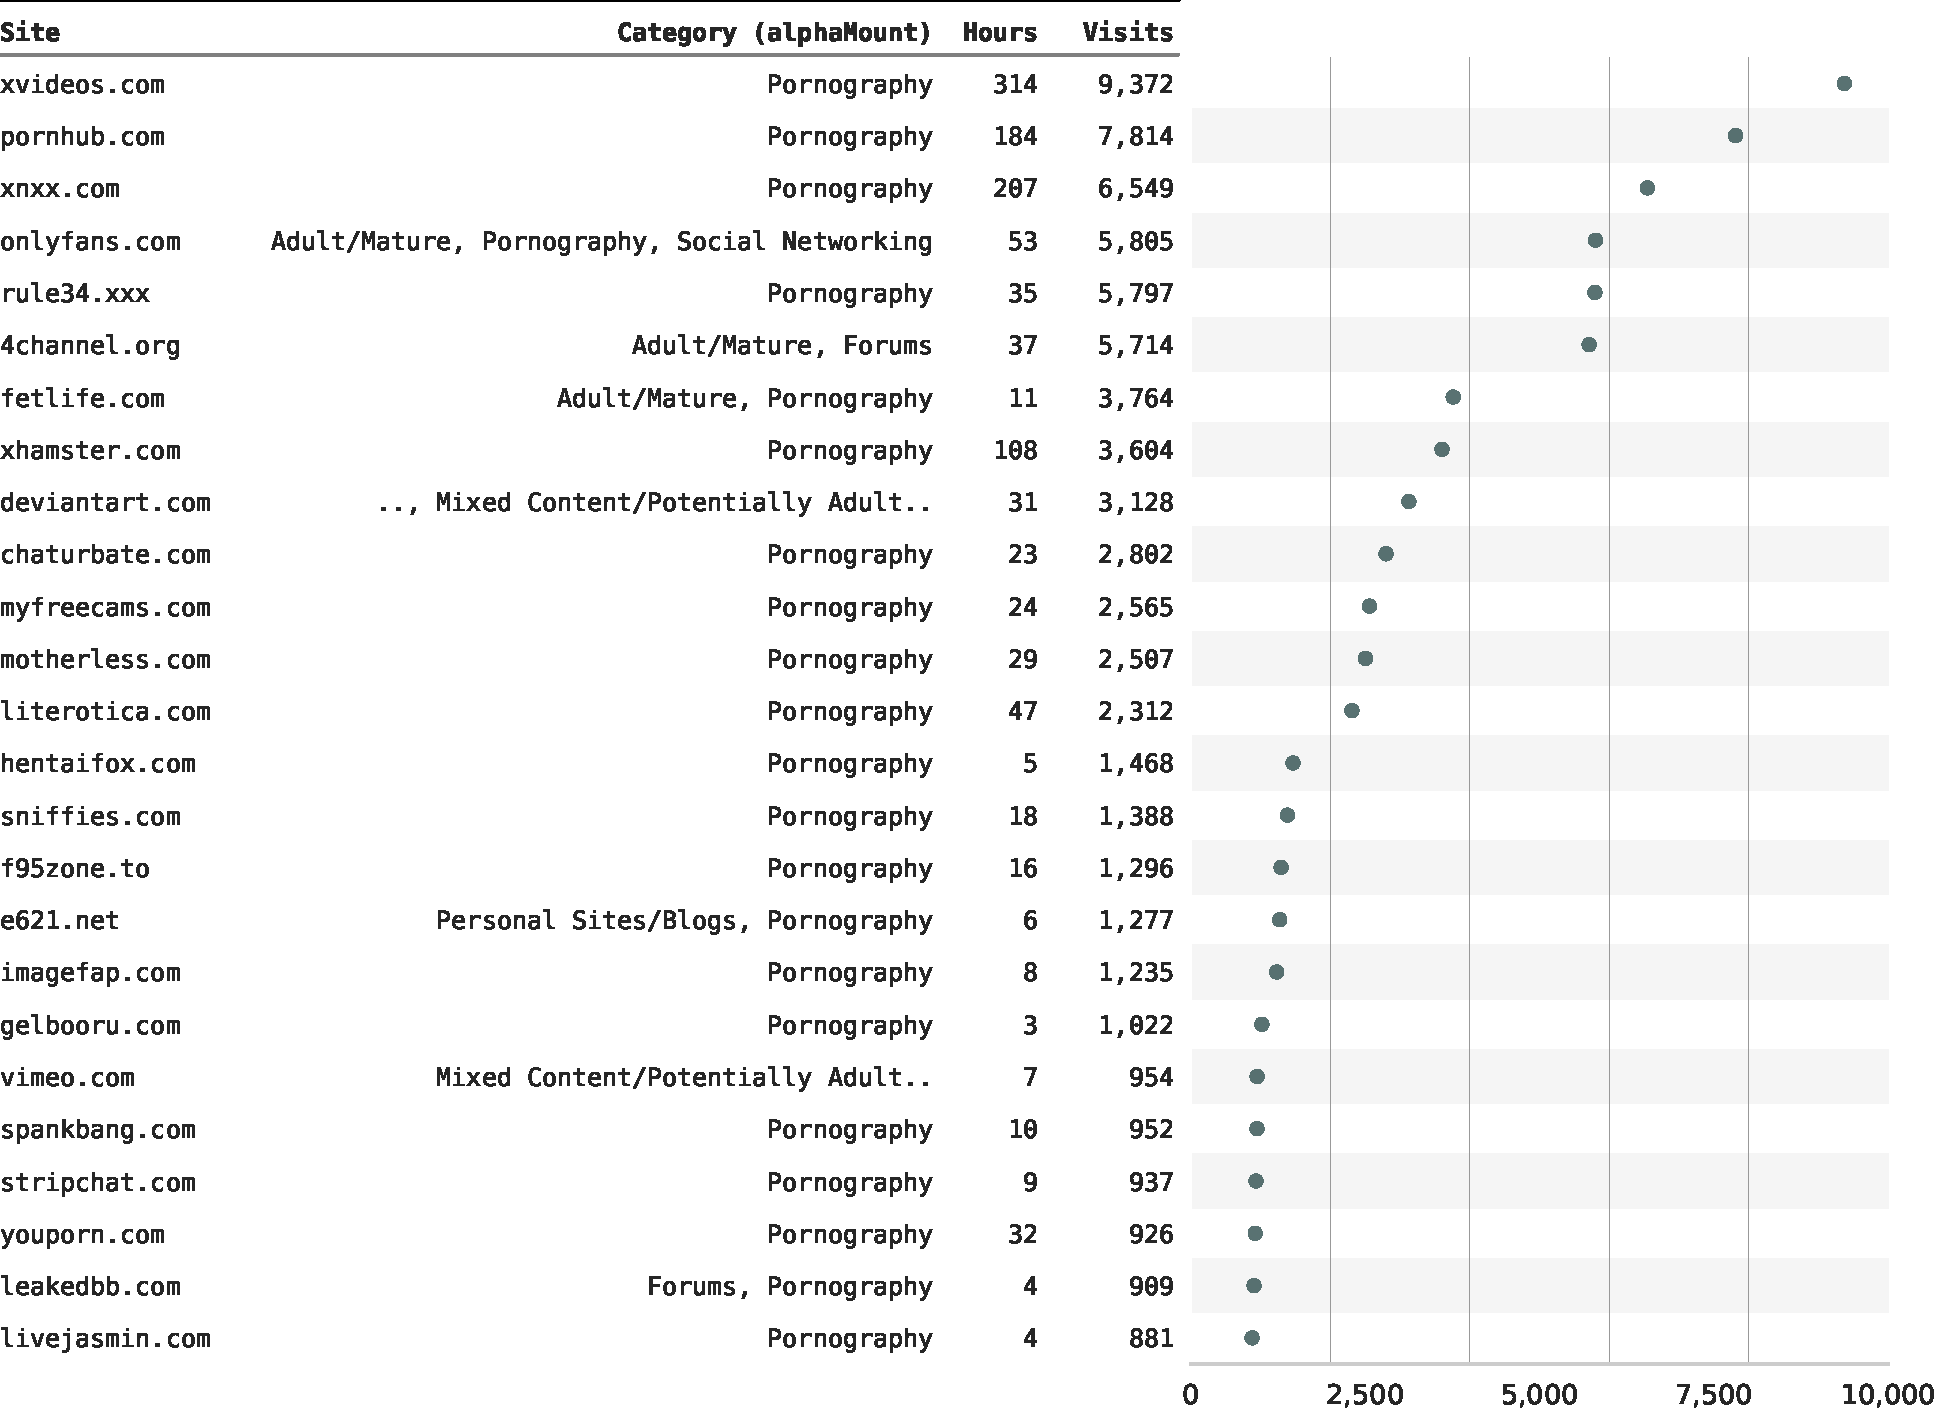
\includegraphics[width=\textwidth]{figs/top_25_adultsites_alphamountain.pdf}
	\caption*{\footnotesize \emph{Notes:} 
		The table shows the top 25 pornographic sites that individuals visited in the sample period.
            All numbers are based on online visits during the one-month period.
		Pornography sites are categorized by alphaMountain (we include any categories mentioning ``porn'', ``adult'' or ``mature'').
            See \cref{fig:top25_adult} for a comparison with our base classification.
    	The \emph{Hours} column is the total number of hours individuals in the sample spent on the site. 
    	The \emph{Visits} column is the total number of visits by individuals in the sample to the site.            
	}
	\label{fig:top25_adult_alphamountain}
\end{figure}

%===========================

% Quantile regressions

% Hours spent on adult sites

%===========================

\begin{figure}[t]
	\centering
	\caption{Distribution of Partisan Differences in Hours Spent on Pornographic Sites (alphaMountain)}
	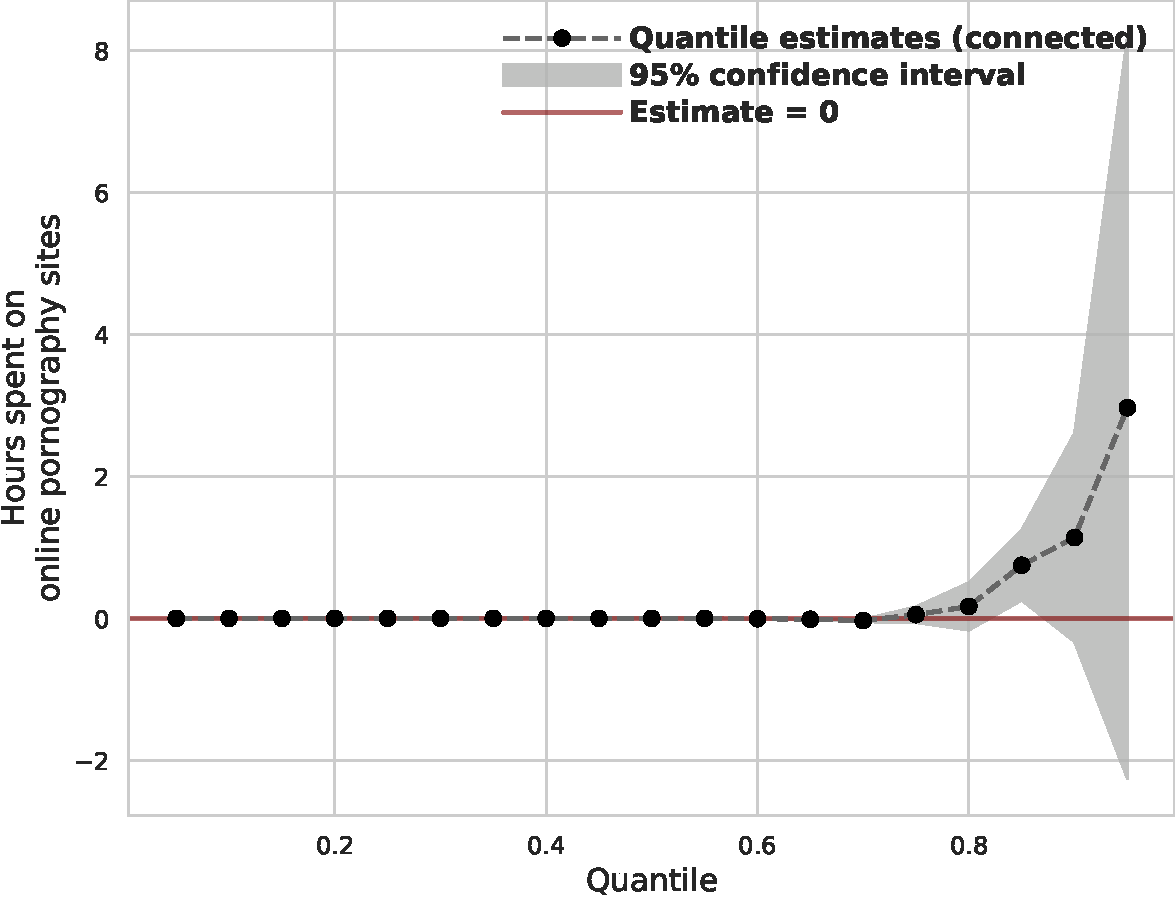
\includegraphics[width=.7\linewidth]{figs/alphamountain_quantile_reg_duration_adult.pdf}
	\caption*{\footnotesize \emph{Notes:} 
		The dependent variable is the number of hours individuals in our sample spent on pornographic sites.
		Each point indicates the difference between Republicans and Democrats and corresponds to a quantile regression at the quantile indicated by the x-axis.
		95\% confidence intervals constructed from standard errors.
		See \cref{fig:alphamountain_quantile_regression_duration_covariates} for the same plot controlling for individual characteristics.
	}
	\label{fig:alphamountain_quantile_regression_duration}
\end{figure}

%=====================================================
% Fig of quantile regression estimates
% Time Spent on Adult Sites by Party (with covariates) 
%=====================================================
\begin{figure}[ht]
	\centering
	\caption{Quantile Estimates--Hours Spent on Pornographic Sites by Party (with covariates, Bitdefender)}
	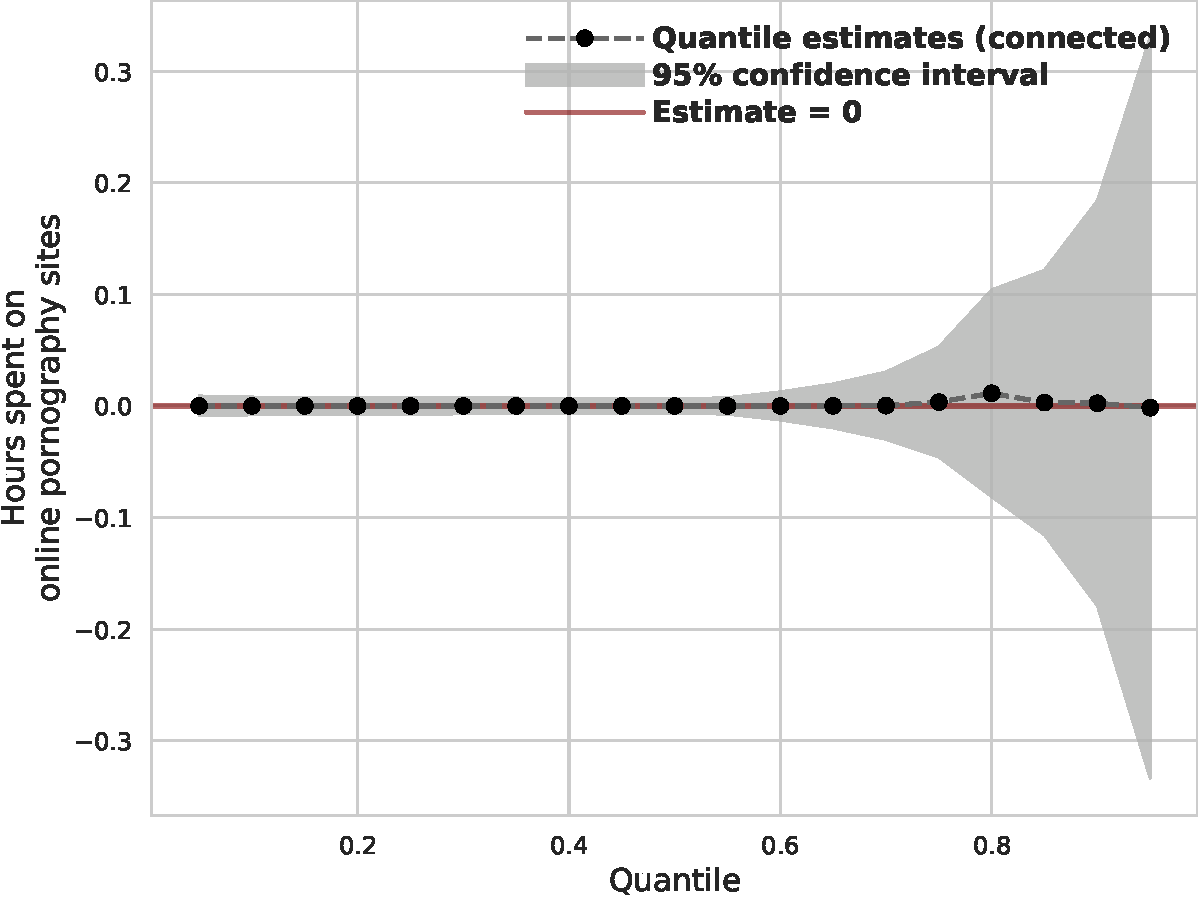
\includegraphics[width=.55\linewidth]{figs/alphamountain_quantile_reg_covariates_duration_adult.pdf}
	\caption*{\footnotesize \emph{Notes:} 
		The dependent variable is the number of hours individuals in our sample spent on pornographic sites. Each point indicates the difference between Republicans and Democrats and corresponds to a quantile regression at the quantile indicated by the x-axis. Covariates included gender (Female/Male), race (White/Black/Hispanic/Asian/Others), education level (no HS/HS graduate/some college/college graduate), age and its quadratic, and region (NE/MW/S/W). 95\% confidence intervals constructed from standard errors. See \cref{fig:alphamountain_quantile_regression_duration_covariates} for the same plot without covariates.
	}
	\label{fig:alphamountain_quantile_regression_duration_covariates}
\end{figure}


\setcounter{table}{0}
\setcounter{figure}{0}
\setcounter{equation}{0}
% =============================================================================
\FloatBarrier
\renewcommand{\thetable}{F\arabic{table}}
\renewcommand{\thefigure}{F\arabic{figure}}
\renewcommand{\theequation}{F\arabic{equation}}
\subsection{F. \smFTitle{}}\label{sm:smF}
% =============================================================================
%===========================================================================
% Tabulated splits by party and by percentiles for hours spent on adultsites
%===========================================================================
\begin{table}[!ht] \centering \small \setlength\tabcolsep{6 pt}
	\caption{Time Spent on Pornographic Sites (including Independents)}
	\label{tab:percentiles_duration_adultsites_by_individuals_independents_partisans}
	\begin{adjustbox}{max width=\textwidth}
		\begin{tabular}{@{\hspace{0\tabcolsep}}lrrrrr@{\hspace{0\tabcolsep}}}
			\toprule		
			&\multicolumn{1}{c}{(1)}&\multicolumn{1}{c}{(2)}&\multicolumn{1}{c}{(3)}&\multicolumn{1}{c}{(4)}&\multicolumn{1}{c}{(5)}\\	
            &\multicolumn{3}{c}{\textbf{Partisans}}&\multicolumn{2}{c}{\textbf{Non-partisans}}\\
            \cmidrule(lr){2-4}\cmidrule(l){5-6}
			\textbf{Percentile}&\multicolumn{1}{c}{\textbf{Republicans}}&\multicolumn{1}{c}{\textbf{Democrats}}&\multicolumn{1}{c}{\textbf{Partisans}}&\multicolumn{1}{c}{\textbf{Independents}}&\textbf{Independents/DK}\\
			\midrule
			0.00 &  0.0 &  0.0 &  0.0 &  0.0 &  0.0 \\
0.10 &  0.1 &  0.0 &  0.0 &  0.0 &  0.0 \\
0.20 &  0.2 &  0.1 &  0.1 &  0.2 &  0.1 \\
0.30 &  0.3 &  0.1 &  0.2 &  0.4 &  0.3 \\
0.40 &  0.7 &  0.2 &  0.3 &  0.7 &  0.6 \\
0.50 &  1.4 &  0.5 &  0.7 &  1.3 &  1.2 \\
0.60 &  2.2 &  0.7 &  1.3 &  2.4 &  2.0 \\
0.70 &  3.0 &  1.5 &  2.2 &  3.1 &  2.8 \\
0.80 &  5.5 &  2.7 &  4.3 &  6.5 &  4.6 \\
0.90 & 11.2 &  7.0 &  9.7 & 14.0 & 12.0 \\
0.95 & 25.4 & 13.8 & 19.1 & 22.7 & 20.6 \\
0.96 & 27.1 & 18.3 & 21.4 & 24.7 & 23.2 \\
0.97 & 27.9 & 19.9 & 26.0 & 26.7 & 26.4 \\
0.98 & 30.0 & 22.0 & 29.4 & 27.4 & 27.6 \\
0.99 & 36.5 & 46.0 & 37.1 & 33.3 & 43.8 \\
1.00 & 37.5 & 90.5 & 90.5 & 44.3 & 94.0 \\
            \midrule
            Observations&\multicolumn{1}{r}{\text{98}}&\multicolumn{1}{r}{\text{158}}&\multicolumn{1}{r}{\text{256}}&\multicolumn{1}{r}{\text{68}}&105\\   
			\bottomrule
		\end{tabular}
	\end{adjustbox}
	\caption*{\footnotesize \emph{Notes:} 
		The table shows splits by partisans and non-partisans, by key percentiles (each of the ten deciles plus quantiles at the right tail) for the duration (hours) spent by individuals who consumed pornography in the sample period. 
	}
\end{table}

\begin{table}[ht] \centering \small \setlength\tabcolsep{6 pt}
	\caption{Percentage of Time Spent on Pornographic Sites  (including Independents)}
	\label{tab:percentiles_prop_duration_adultsites_by_individuals_independents_partisans}
	\begin{adjustbox}{max width=\textwidth}
		\begin{tabular}{@{\hspace{0\tabcolsep}}lrrrrr@{\hspace{0\tabcolsep}}}
			\toprule		
			&\multicolumn{1}{c}{(1)}&\multicolumn{1}{c}{(2)}&\multicolumn{1}{c}{(3)}&\multicolumn{1}{c}{(4)}&\multicolumn{1}{c}{(5)}\\	
            &\multicolumn{3}{c}{\textbf{Partisans}}&\multicolumn{2}{c}{\textbf{Non-partisans}}\\
            \cmidrule(lr){2-4}\cmidrule(l){5-6}
			\textbf{Percentile}&\multicolumn{1}{c}{\textbf{Republicans}}&\multicolumn{1}{c}{\textbf{Democrats}}&\multicolumn{1}{c}{\textbf{Partisans}}&\multicolumn{1}{c}{\textbf{Independents}}&\textbf{Independents/DK}\\
			\midrule
            0.00 &  0.0 &  0.0 &  0.0 &  0.0 &  0.0 \\
0.10 &  0.1 &  0.0 &  0.0 &  0.0 &  0.0 \\
0.20 &  0.2 &  0.1 &  0.1 &  0.4 &  0.3 \\
0.30 &  0.7 &  0.2 &  0.5 &  1.3 &  1.0 \\
0.40 &  1.7 &  0.8 &  1.0 &  2.4 &  2.0 \\
0.50 &  3.6 &  1.3 &  2.1 &  3.4 &  3.4 \\
0.60 &  6.3 &  3.0 &  4.0 &  6.8 &  6.5 \\
0.70 & 10.5 &  5.5 &  7.1 &  9.5 &  9.8 \\
0.80 & 20.5 & 11.7 & 13.5 & 14.3 & 14.2 \\
0.90 & 36.5 & 35.0 & 36.3 & 31.5 & 33.0 \\
0.95 & 45.1 & 52.8 & 52.4 & 66.1 & 63.4 
% 0.96 & 53.7 & 58.0 & 58.3 & 68.5 & 64.0 \\
% 0.97 & 62.7 & 63.9 & 63.9 & 69.8 & 67.4 \\
% 0.98 & 68.5 & 65.0 & 68.0 & 72.2 & 69.7 \\
% 0.99 & 71.4 & 72.7 & 73.0 & 77.8 & 73.3 \\
% 1.00 & 87.5 & 77.4 & 87.5 & 86.5 & 86.5 \\
            \midrule
            Observations&\multicolumn{1}{r}{\text{98}}&\multicolumn{1}{r}{\text{158}}&\multicolumn{1}{r}{\text{256}}&\multicolumn{1}{r}{\text{68}}&105\\
			\bottomrule
		\end{tabular}
	\end{adjustbox}
	\caption*{\footnotesize \emph{Notes:} The table shows splits by partisans and non-partisans, by key percentiles (each of the ten deciles plus quantiles at the right tail) for the percentage of time spent on pornography by individuals who consumed pornography in the sample period. 
	}
\end{table}

\clearpage
\setcounter{table}{0}
\setcounter{figure}{0}
\setcounter{equation}{0}
% =============================================================================
\FloatBarrier
\renewcommand{\thetable}{G\arabic{table}}
\renewcommand{\thefigure}{G\arabic{figure}}
\renewcommand{\theequation}{G\arabic{equation}}
\subsection{G. \smGTitle{}}\label{sm:smG}
% =============================================================================
\subsubsection{Proportion of the Group That Consumed Any Pornography}
%============================================================================
% Figure of porn consumption by party
% Y-axis = proportion of individuals that ever consumed porn in sample period
%============================================================================
\begin{figure}[ht]
	\centering
	\caption{Pornography Consumption by Party}
	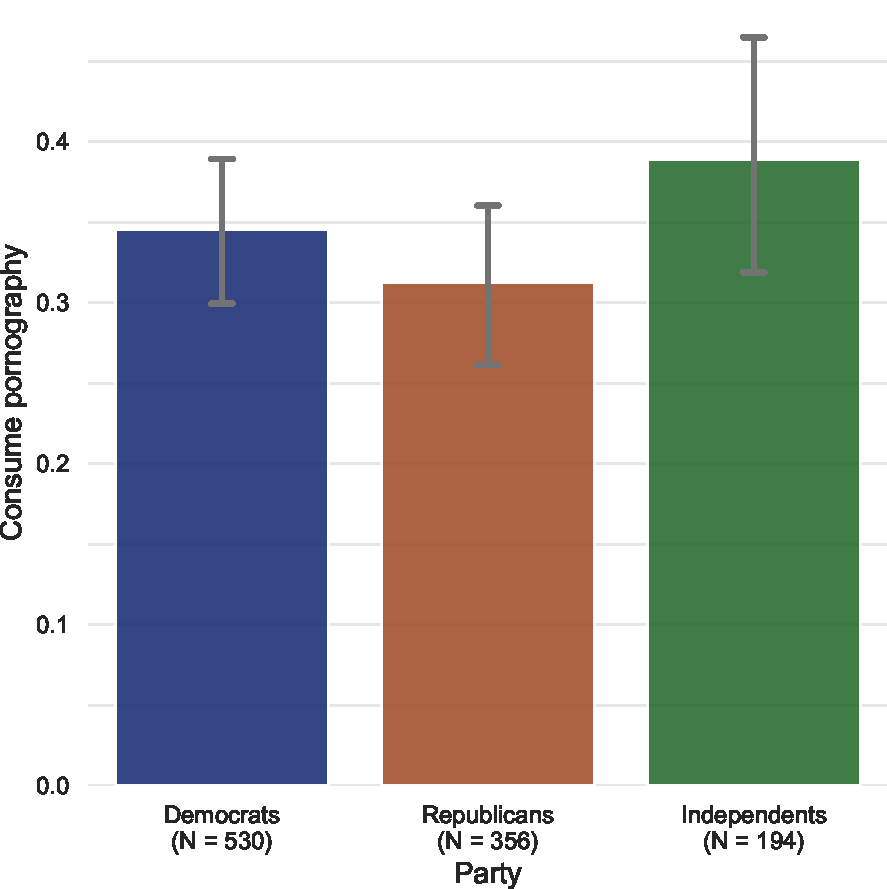
\includegraphics[width=.5\textwidth]{figs/consume_porn_yes_no.pdf}
	\caption*{\footnotesize \emph{Notes:} 
		The figure shows the proportion of individuals in the sample who consumed pornography in the sample period by party.
		Capped vertical bars are 95\% confidence intervals from bootstrapped standard errors (n = 1,000).
	}
	\label{fig:consume_porn_yes_no}
\end{figure}
\clearpage

\FloatBarrier
%===============================================================================
%===============================================================================
% Analogous results for visits to adult sites
%===============================================================================
%===============================================================================
\subsubsection{Analyses of Visits}
\label{si:visits}
%=================================================
% Figure for Distribution of visits to adult sites
%=================================================
\begin{figure}[ht]
	\centering
	\caption{Distribution of Traffic to Pornography Online}
	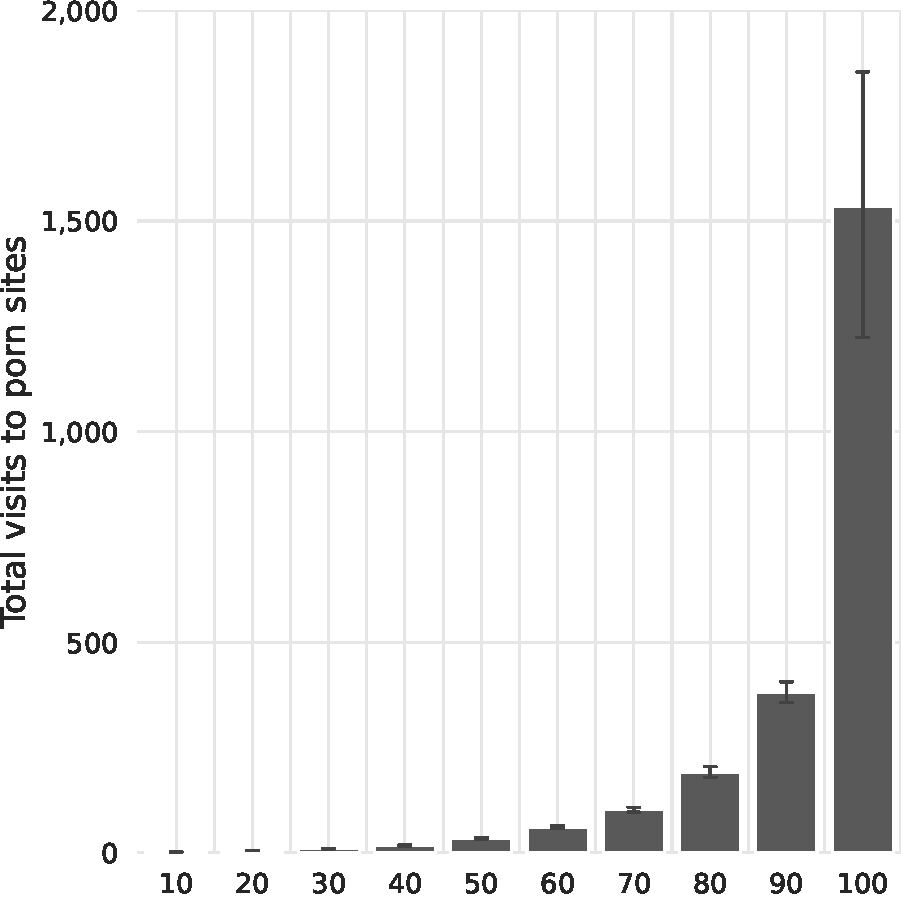
\includegraphics[width=.5\linewidth]{figs/distribution_visits_to_adultsites.pdf}
	\caption*{\footnotesize \emph{Notes:} 
		The figure shows the number of visits to pornography sites by individuals who consumed pornography in the sample period.
		Individuals are split into deciles, with each bin containing approximately the same number of individuals.
		The height of the bars indicates the mean of each bin.
		Capped vertical bars are 95\% confidence intervals.
		%See \cref{tab:distribution_visits} for the more tabulated values.
	}
	\label{fig:distribution_visits}
\end{figure}




%===============================================================
% Figure for Distribution of proportion of visits to adult sites
%===============================================================
\begin{figure}
	\centering
	\caption{Percentage of Traffic to Pornography Online}
	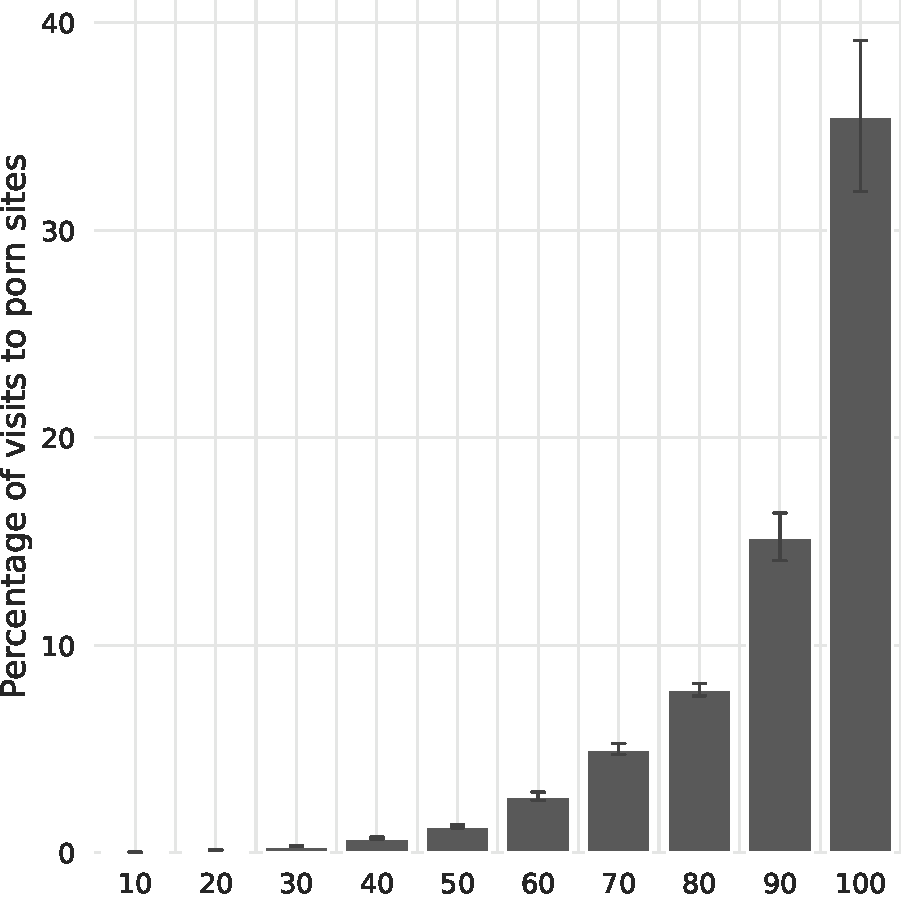
\includegraphics[width=.5\linewidth]{figs/distribution_proportion_visits_to_adultsites.pdf}
	\caption*{\footnotesize \emph{Notes:} 
		The figure shows the proportion of visits to pornography sites by individuals who consumed pornography in the sample period.
		Individuals are split into deciles, with each bin containing approximately the same number of individuals.
		The height of the bars indicates the mean of each bin.
		Capped vertical bars are 95\% confidence intervals.
		%See \cref{tab:distribution_prop_visits} for the more tabulated values.
	}
	\label{fig:distribution_prop_visits}
\end{figure}


\begin{table}[ht] \centering \small \setlength\tabcolsep{10 pt}
	\caption{Distribution of Consumption of Pornography Online by Party}
	\label{tab:distribution_visits_party}
	\begin{adjustbox}{max width=\textwidth}
		\begin{tabular}{crr}
			\toprule
			\multicolumn{1}{l}{\textbf{}}&\multicolumn{2}{c}{\textbf{Traffic}}\\
			\cmidrule(l){2-3}
			\multicolumn{1}{l}{\textbf{Percentile}}&\multicolumn{1}{c}{\textbf{Republicans}}&\multicolumn{1}{c}{\textbf{Democrats}}\\
			\midrule
		%percentiles_duration_adultsites_by_individuals_by_party
            0.00 &     1 &     1 \\
0.10 &     4 &     2 \\
0.20 &     9 &     5 \\
0.30 &    15 &     9 \\
0.40 &    48 &    14 \\
0.50 &    82 &    25 \\
0.60 &   125 &    39 \\
0.70 &   210 &    82 \\
0.80 &   310 &   157 \\
0.90 &   566 &   452 \\
0.95 &   863 & 1,246 \\
0.96 & 1,235 & 1,425 \\
0.97 & 1,539 & 1,503 \\
0.98 & 2,348 & 1,875 \\
0.99 & 2,414 & 2,465 \\
1.00 & 2,560 & 3,980 \\
			\bottomrule
		\end{tabular}
	\end{adjustbox}
	\caption*{\footnotesize \emph{Notes:} 
		The table shows splits by party and key percentiles (each of the ten deciles plus quantiles at the right tail) for the visits to pornographic sites.
		See \cref{tab:distribution_duration_party} for the distribution in terms of time spent. 
		See \cref{fig:distribution_visits} for the plot.
	}
\end{table}


\begin{table}[ht] \centering \small \setlength\tabcolsep{10 pt}
	\caption{Distribution of Consumption of Pornography Online by Party}
	\label{tab:distribution_prop_visits_party}
	\begin{adjustbox}{max width=\textwidth}
		\begin{tabular}{crr}
			\toprule
			\multicolumn{1}{l}{\textbf{}}&\multicolumn{2}{c}{\textbf{\% Traffic}}\\
			\cmidrule(l){2-3}
			\multicolumn{1}{l}{\textbf{Percentile}}&\multicolumn{1}{c}{\textbf{Republicans}}&\multicolumn{1}{c}{\textbf{Democrats}}\\
			\midrule
		%percentiles_duration_adultsites_by_individuals_by_party
            0.00 &  0.0 &  0.0 \\
0.10 &  0.1 &  0.1 \\
0.20 &  0.4 &  0.1 \\
0.30 &  0.8 &  0.3 \\
0.40 &  1.4 &  0.5 \\
0.50 &  2.8 &  1.0 \\
0.60 &  4.3 &  1.9 \\
0.70 &  7.7 &  4.6 \\
0.80 & 16.0 &  7.0 \\
0.90 & 21.1 & 18.8 \\
0.95 & 30.5 & 27.4 
% 0.96 & 32.7 & 29.9 \\
% 0.97 & 42.6 & 33.6 \\
% 0.98 & 46.5 & 38.6 \\
% 0.99 & 52.8 & 42.4 \\
% 1.00 & 53.5 & 59.9 \\
			\bottomrule
		\end{tabular}
	\end{adjustbox}
	\caption*{\footnotesize \emph{Notes:} 
		The table shows splits by party and by key percentiles (each of the ten deciles plus quantiles at the right tail) for the duration (hours) spent by individuals who consumed pornography in the sample period. 
		See \cref{tab:distribution_prop_duration_party} for the distribution in terms of percentage of time. 
		See \cref{fig:distribution_prop_visits} for the plot.
	}
\end{table}

\FloatBarrier
%=======================
% Quantile regressions
% Traffic to adult sites
%=======================
\begin{figure}
	\centering
	\caption{Quantile Estimates--Traffic to Pornography Sites by Party}
	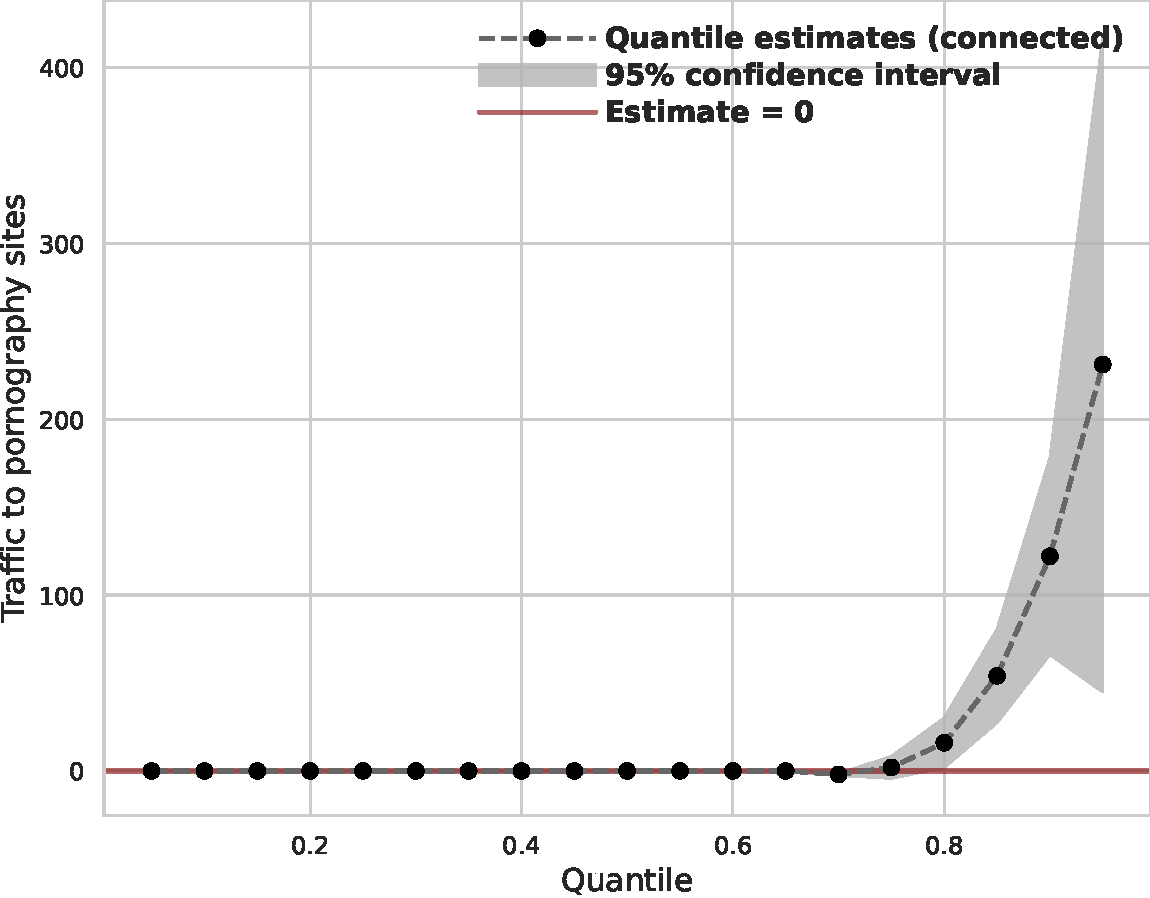
\includegraphics[width=.55\linewidth]{figs/quantile_reg_visits_adult.pdf}
	\caption*{\footnotesize \emph{Notes:} 
		The dependent variable is the number of visits to pornographic sites by individuals in our sample.
		Each point indicates the difference between Republicans and Democrats and corresponds to a quantile regression at the quantile indicated by the x-axis.
		95\% confidence intervals constructed from standard errors.
		See \cref{fig:quantile_regression_visits_covariates} for the same plot controlling for individual characteristics.
            \cref{tab:quantile-estimates-traffic} tabulates the estimates.
	}
	\label{fig:quantile_regression_visits}
\end{figure}

%==================================================
% Fig of quantile regression estimates
% Traffic to Adult Sites by Party (with covariates) 
%==================================================
\begin{figure}
	\centering
	\caption{Quantile Estimates--Traffic to Pornographic Sites by Party (with covariates)}
	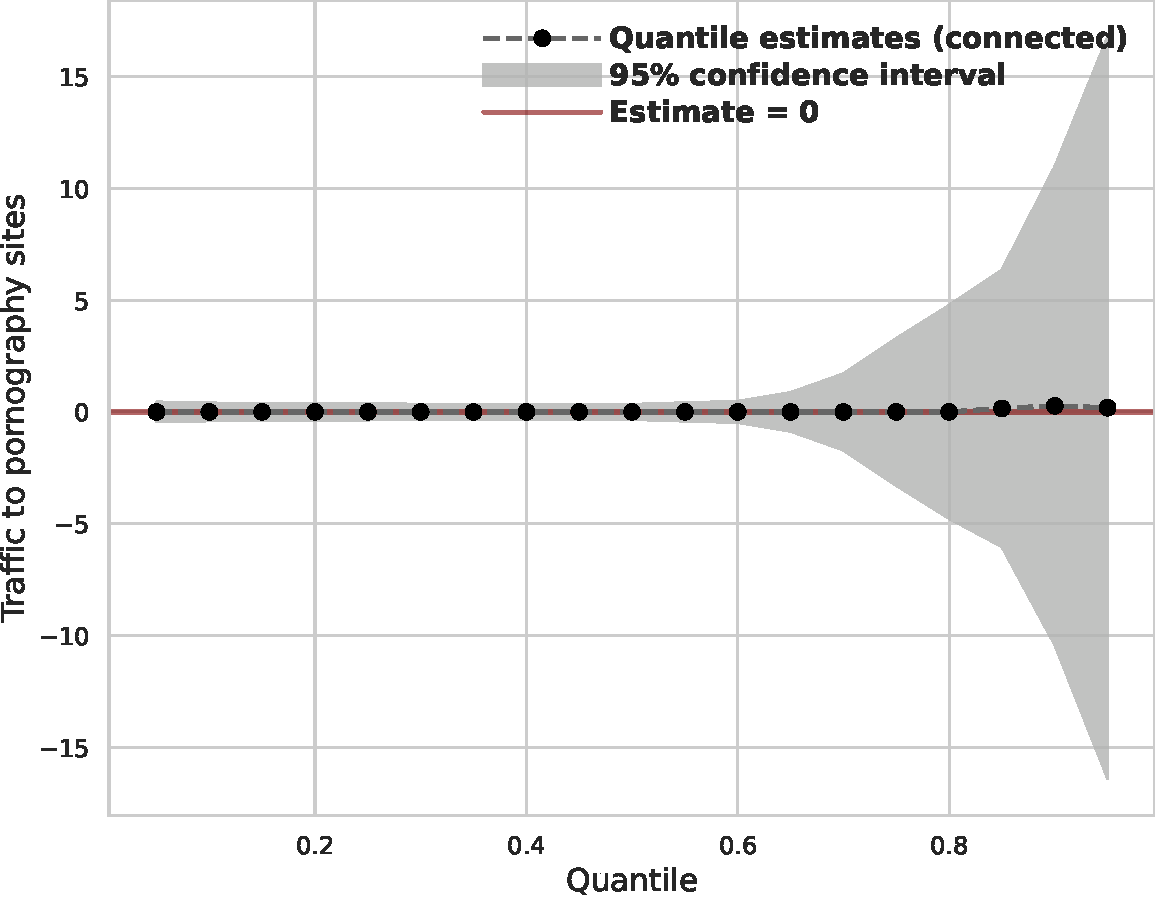
\includegraphics[width=.55\linewidth]{figs/quantile_reg_covariates_visits_adult.pdf}
	\caption*{\footnotesize \emph{Notes:} 
		The dependent variable is the number of visits to pornographic sites by individuals in our sample.
		Each point indicates the difference between Republicans and Democrats and corresponds to a quantile regression at the quantile indicated by the x-axis.
		Covariates included on the right-hand side are gender (Female/Male), race (White/Black/Hispanic/Asian/Others), education level (no HS/HS graduate/some college/college graduate), age and its quadratic, and region (NE/MW/S/W).
		95\% confidence intervals constructed from standard errors.
		See \cref{fig:quantile_regression_visits} for the same plot without covariates.
            \cref{tab:quantile-estimates-traffic} tabulates the estimates.
	}
	\label{fig:quantile_regression_visits_covariates}
\end{figure}

%=====================================
% Quantile regressions
% Proportion of traffic to adult sites
%=====================================
\begin{figure}
	\centering
	\caption{Quantile Estimates--Percentage of Traffic to Pornographic Sites by Party}
	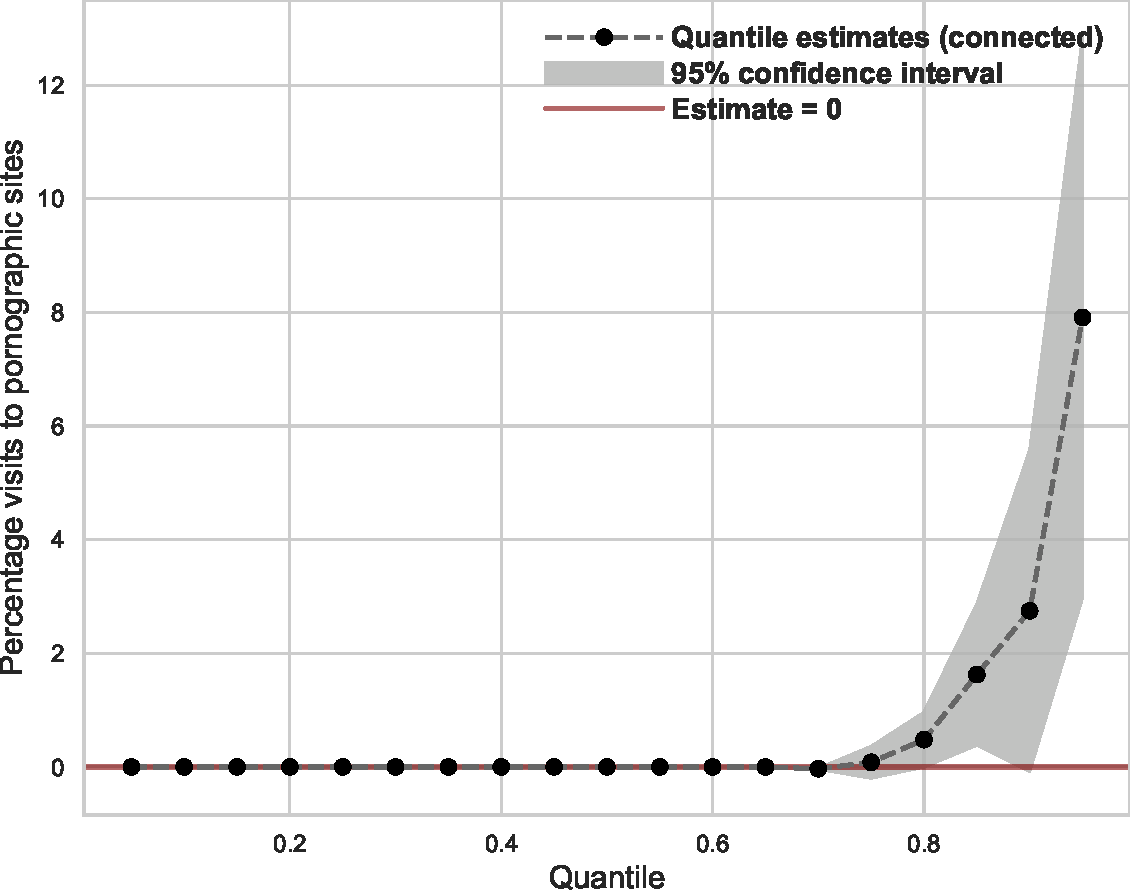
\includegraphics[width=.55\linewidth]{figs/quantile_reg_proportion_visits_adult.pdf}
	\caption*{\footnotesize \emph{Notes:} 
		The dependent variable is the percentage of traffic to pornographic sites by individuals in our sample.
		Each point indicates the difference between Republicans and Democrats and corresponds to a quantile regression at the quantile indicated by the x-axis.
		95\% confidence intervals constructed from standard errors.
		See \cref{fig:quantile_regression_prop_visits_covariates} for the same plot controlling for individual characteristics.
            \cref{tab:quantile-estimates-prop-traffic} tabulates the estimates.
	}
	\label{fig:quantile_regression_prop_visits}
\end{figure}

%=============================================================
% Fig of quantile regression estimates
% Percentage Traffic to Adult Sites by Party (with covariates) 
%=============================================================
\begin{figure}
	\centering
	\caption{Quantile Estimates--Percentage of Traffic to Pornographic Sites by Party (with covariates)}
	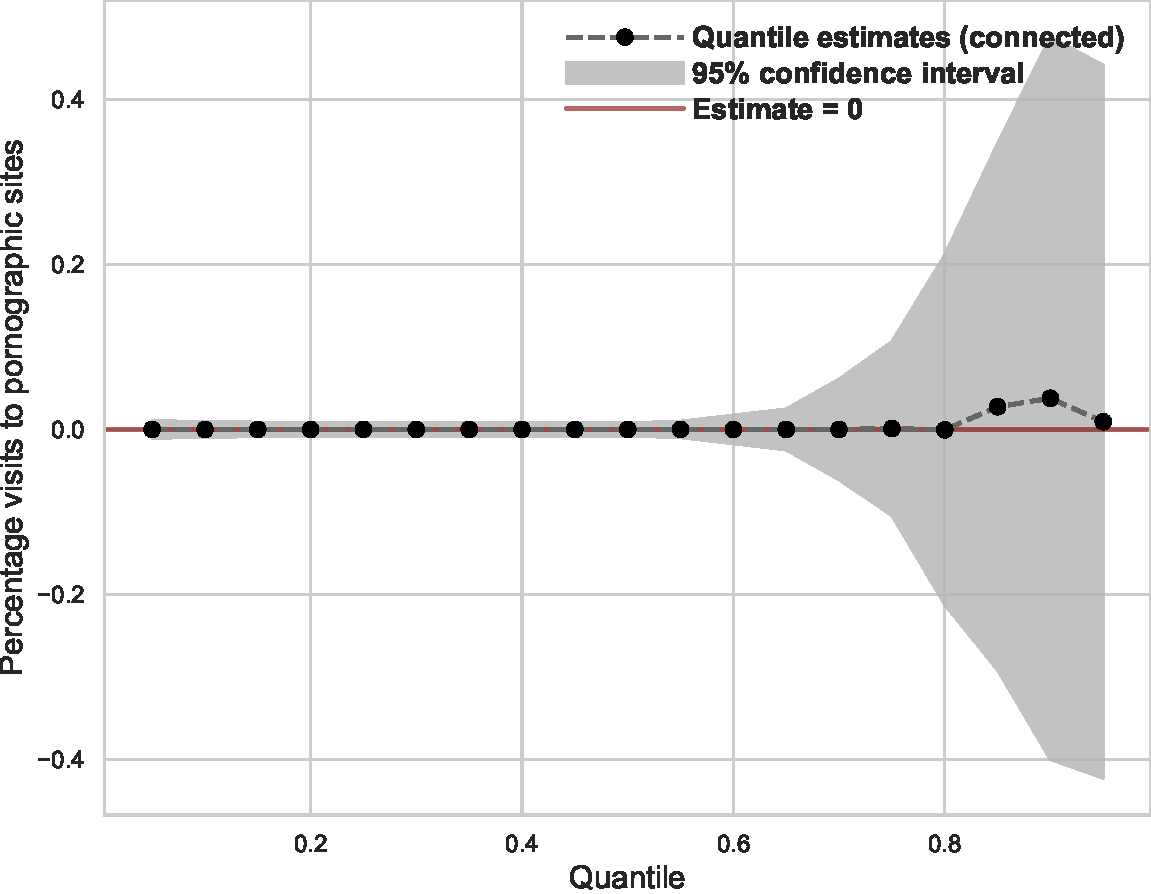
\includegraphics[width=.55\linewidth]{figs/quantile_reg_covariates_proportion_visits_adult.pdf}
	\caption*{\footnotesize \emph{Notes:} 
		The dependent variable is the percentage of traffic to pornographic sites by individuals in our sample.
		Each point indicates the difference between Republicans and Democrats and corresponds to a quantile regression at the quantile indicated by the x-axis.
		Covariates included on the right-hand side are gender (Female/Male), race (White/Black/Hispanic/Asian/Others), education level (no HS/HS graduate/some college/college graduate), age and its quadratic, and region (NE/MW/S/W).
		95\% confidence intervals constructed from standard errors.
		See \cref{fig:quantile_regression_prop_visits} for the same plot without covariates.
            \cref{tab:quantile-estimates-prop-traffic} tabulates the estimates.
	}
	\label{fig:quantile_regression_prop_visits_covariates}
\end{figure}


\begin{landscape}% Landscape page
    \begin{table}[ht] \centering \ssmall \setlength\tabcolsep{0 pt} \setlength{\defaultaddspace}{0pt}
    \def\sym#1{\ifmmode^{#1}\else\(^{#1}\)\fi}
    \caption{Quantile Estimates--Traffic to Pornographic Sites by Party }
    \label{tab:quantile-estimates-traffic}
	\begin{adjustbox}{max width=1.325\textwidth}
            \begin{tabular}{l*{20}{D{.}{.}{-1}}}
            \toprule\toprule
            &\multicolumn{1}{c}{(1)}         &\multicolumn{1}{c}{(2)}         &\multicolumn{1}{c}{(3)}         &\multicolumn{1}{c}{(4)}         &\multicolumn{1}{c}{(5)}         &\multicolumn{1}{c}{(6)}         &\multicolumn{1}{c}{(7)}         &\multicolumn{1}{c}{(8)}         &\multicolumn{1}{c}{(9)}         &\multicolumn{1}{c}{(10)}&\multicolumn{1}{c}{(11)}         &\multicolumn{1}{c}{(12)}         &\multicolumn{1}{c}{(13)}         &\multicolumn{1}{c}{(14)}         &\multicolumn{1}{c}{(15)}         &\multicolumn{1}{c}{(16)}         &\multicolumn{1}{c}{(17)}         &\multicolumn{1}{c}{(18)}         &\multicolumn{1}{c}{(19)}         &\multicolumn{1}{c}{(20)}         \\
            \cmidrule(l){2-21}
            % ===================================================================
            % Panel A
            &\multicolumn{20}{c}{\textbf{Panel A. Unconditional quantile estimates}}\\
            &\multicolumn{1}{c}{p5}         &\multicolumn{1}{c}{p10}         &\multicolumn{1}{c}{p15}         &\multicolumn{1}{c}{p20}         &\multicolumn{1}{c}{p25}         &\multicolumn{1}{c}{p30}         &\multicolumn{1}{c}{p35}         &\multicolumn{1}{c}{p40}         &\multicolumn{1}{c}{p45}         &\multicolumn{1}{c}{p50}&\multicolumn{1}{c}{p55}         &\multicolumn{1}{c}{p60}         &\multicolumn{1}{c}{p65}         &\multicolumn{1}{c}{p70}         &\multicolumn{1}{c}{p75}         &\multicolumn{1}{c}{p80}         &\multicolumn{1}{c}{p85}         &\multicolumn{1}{c}{p90}         &\multicolumn{1}{c}{p95}         &\multicolumn{1}{c}{p100}         \\
            \cmidrule(l){2-21}
             Republican & 13.83 & -0.00 & -0.00 & -0.00 & -0.00 & -0.00 & -0.00 & -0.00 & -0.00 & -0.00 & -0.00 & -0.00 & -0.00 & -0.00 & -2.00\sym{a} & 2.00 & 16.00\sym{b} & 54.00\sym{a} & 122.00\sym{a} & 231.00\sym{b} \\
& (20.00) & (0.22) & (0.20) & (0.19) & (0.18) & (0.18) & (0.17) & (0.17) & (0.17) & (0.16) & (0.16) & (0.15) & (0.14) & (0.14) & (0.26) & (3.16) & (7.16) & (13.49) & (28.45) & (94.81) \\
 Constant & 59.87\sym{a} & 0.00 & 0.00 & 0.00 & 0.00 & 0.00 & 0.00 & 0.00 & 0.00 & 0.00 & 0.00 & 0.00 & 0.00 & 0.00 & 2.00\sym{a} & 6.00\sym{a} & 12.00\sym{a} & 28.00\sym{a} & 60.00\sym{a} & 222.00\sym{a} \\
& (13.37) & (0.14) & (0.12) & (0.12) & (0.11) & (0.11) & (0.11) & (0.11) & (0.11) & (0.10) & (0.10) & (0.10) & (0.09) & (0.09) & (0.17) & (2.00) & (4.52) & (8.52) & (17.86) & (60.19) \\
            \cmidrule(l){2-21}
            % ===================================================================
            % Panel B            
            &\multicolumn{20}{c}{\textbf{Panel B. Adjusted quantile estimates}}\\
            &\multicolumn{1}{c}{p5}         &\multicolumn{1}{c}{p10}         &\multicolumn{1}{c}{p15}         &\multicolumn{1}{c}{p20}         &\multicolumn{1}{c}{p25}         &\multicolumn{1}{c}{p30}         &\multicolumn{1}{c}{p35}         &\multicolumn{1}{c}{p40}         &\multicolumn{1}{c}{p45}         &\multicolumn{1}{c}{p50}&\multicolumn{1}{c}{p55}         &\multicolumn{1}{c}{p60}         &\multicolumn{1}{c}{p65}         &\multicolumn{1}{c}{p70}         &\multicolumn{1}{c}{p75}         &\multicolumn{1}{c}{p80}         &\multicolumn{1}{c}{p85}         &\multicolumn{1}{c}{p90}         &\multicolumn{1}{c}{p95}         &\multicolumn{1}{c}{p100}         \\  
            \cmidrule(l){2-21}
              Republican & 5.10 & -0.00 & -0.00 & -0.00 & -0.00 & -0.00 & -0.00 & -0.00 & -0.00 & -0.00 & -0.00 & -0.00 & -0.00 & 0.00 & 0.00 & 0.00 & 0.00 & 0.16 & 0.27 & 0.19 \\
& (20.28) & (0.23) & (0.20) & (0.19) & (0.19) & (0.18) & (0.18) & (0.18) & (0.18) & (0.17) & (0.17) & (0.21) & (0.24) & (0.44) & (0.87) & (1.67) & (2.42) & (3.15) & (5.44) & (8.44) \\
 Female & -105.18\sym{a} & -0.00 & -0.00 & -0.00 & -0.00 & -0.00 & -0.00 & -0.00 & -0.00 & -0.00 & -0.00 & -3.00\sym{a} & -7.00\sym{a} & -13.00\sym{a} & -29.00\sym{a} & -54.00\sym{a} & -88.00\sym{a} & -127.89\sym{a} & -269.04\sym{a} & -532.08\sym{a} \\
& (21.43) & (0.20) & (0.18) & (0.17) & (0.17) & (0.16) & (0.16) & (0.16) & (0.16) & (0.16) & (0.16) & (0.19) & (0.22) & (0.40) & (0.80) & (1.52) & (2.21) & (2.90) & (5.02) & (7.51) \\
 Educ (HS) & 33.55 & 0.00 & 0.00 & 0.00 & 0.00 & 0.00 & 0.00 & 0.00 & 0.00 & 0.00 & 0.00 & 0.00 & 0.00 & 0.00 & 0.00 & 0.00 & 0.00 & 0.08 & 0.01 & 0.42 \\
& (26.53) & (0.51) & (0.46) & (0.43) & (0.42) & (0.41) & (0.41) & (0.40) & (0.40) & (0.39) & (0.39) & (0.48) & (0.55) & (1.02) & (1.99) & (3.92) & (5.94) & (7.78) & (13.76) & (19.51) \\
 Educ (some coll.) & 67.73\sym{c} & 0.00 & 0.00 & 0.00 & 0.00 & 0.00 & 0.00 & 0.00 & 0.00 & 0.00 & 0.00 & 0.00 & 0.00 & 0.00 & 0.00 & 4.00 & 10.00\sym{c} & 12.40 & 21.76 & 62.17\sym{a} \\
& (39.41) & (0.52) & (0.47) & (0.44) & (0.43) & (0.42) & (0.42) & (0.41) & (0.41) & (0.40) & (0.40) & (0.49) & (0.56) & (1.04) & (2.04) & (4.00) & (6.04) & (7.95) & (13.96) & (19.76) \\
 Educ (coll. grad.) & 17.42 & -0.00 & -0.00 & -0.00 & -0.00 & -0.00 & 0.00 & 0.00 & 0.00 & 0.00 & 0.00 & 0.00 & 0.00 & 0.00 & 0.00 & 0.00 & 0.00 & -0.05 & 0.12 & 0.40 \\
& (23.59) & (0.50) & (0.44) & (0.42) & (0.41) & (0.40) & (0.40) & (0.39) & (0.39) & (0.38) & (0.38) & (0.47) & (0.54) & (1.00) & (1.95) & (3.83) & (5.82) & (7.59) & (13.41) & (19.24) \\
 Age & 0.20 & -0.00 & -0.00 & -0.00 & -0.00 & -0.00 & -0.00 & -0.00 & -0.00 & -0.00 & -0.00 & -0.00 & -0.00 & -0.00 & -0.00 & -0.00 & -0.00 & -1.13\sym{b} & -1.86\sym{b} & -3.30\sym{a} \\
& (3.10) & (0.03) & (0.03) & (0.03) & (0.03) & (0.03) & (0.03) & (0.03) & (0.03) & (0.03) & (0.03) & (0.03) & (0.04) & (0.07) & (0.13) & (0.25) & (0.36) & (0.45) & (0.77) & (1.07) \\
 Age$^2$ & -0.01 & -0.00 & -0.00 & -0.00 & -0.00 & -0.00 & -0.00 & -0.00 & -0.00 & -0.00 & -0.00 & 0.00 & 0.00 & 0.00 & 0.00 & 0.00 & 0.00 & 0.01\sym{c} & 0.01\sym{c} & 0.02\sym{b} \\
& (0.03) & (0.00) & (0.00) & (0.00) & (0.00) & (0.00) & (0.00) & (0.00) & (0.00) & (0.00) & (0.00) & (0.00) & (0.00) & (0.00) & (0.00) & (0.00) & (0.00) & (0.00) & (0.01) & (0.01) \\
 Race (Black) & 13.40 & 0.00 & 0.00 & 0.00 & 0.00 & 0.00 & 0.00 & 0.00 & 0.00 & 0.00 & 0.00 & 0.00 & 0.00 & 0.00 & 1.00 & 2.00 & 2.00 & 0.19 & 21.80\sym{a} & 203.77\sym{a} \\
& (32.40) & (0.35) & (0.31) & (0.30) & (0.29) & (0.28) & (0.28) & (0.27) & (0.27) & (0.27) & (0.26) & (0.32) & (0.36) & (0.66) & (1.34) & (2.55) & (3.65) & (4.95) & (8.29) & (11.77) \\
 Race (Hispanic) & -19.01 & 0.00 & 0.00 & 0.00 & 0.00 & 0.00 & 0.00 & 0.00 & 0.00 & 0.00 & 0.00 & -0.00 & -0.00 & -0.00 & -0.00 & -0.00 & 0.00 & 0.11 & -0.25 & 7.57 \\
& (26.79) & (0.32) & (0.29) & (0.27) & (0.26) & (0.26) & (0.25) & (0.25) & (0.25) & (0.24) & (0.24) & (0.29) & (0.34) & (0.61) & (1.20) & (2.31) & (3.33) & (4.41) & (7.87) & (9.78) \\
 Race (Asian) & -11.17 & -0.00 & -0.00 & -0.00 & -0.00 & -0.00 & -0.00 & -0.00 & -0.00 & -0.00 & -0.00 & -0.00 & -0.00 & -0.00 & -0.00 & -0.00 & -0.00 & 0.16 & 19.36 & 58.78\sym{a} \\
& (44.78) & (0.45) & (0.40) & (0.38) & (0.38) & (0.38) & (0.38) & (0.39) & (0.39) & (0.40) & (0.41) & (0.52) & (0.61) & (1.13) & (2.15) & (4.09) & (6.17) & (7.53) & (13.94) & (18.88) \\
 Race (Other) & 96.68 & 0.00 & 0.00 & 0.00 & 0.00 & 0.00 & 0.00 & 0.00 & 0.00 & 0.00 & 0.00 & 0.00 & 0.00 & 2.17\sym{b} & 4.00\sym{b} & 54.00\sym{a} & 154.00\sym{a} & 219.16\sym{a} & 113.14\sym{a} & 0.32 \\
& (80.50) & (0.52) & (0.46) & (0.44) & (0.43) & (0.42) & (0.42) & (0.41) & (0.41) & (0.41) & (0.40) & (0.49) & (0.56) & (1.03) & (2.02) & (3.93) & (5.69) & (7.39) & (13.65) & (17.72) \\
 Region (MW) & 107.04\sym{a} & 0.00 & 0.00 & 0.00 & 0.00 & 0.00 & 0.00 & 0.00 & 0.00 & 0.00 & 0.00 & 3.00\sym{a} & 7.00\sym{a} & 2.17 & 5.80 & 54.00\sym{a} & 88.00\sym{a} & 31.90\sym{c} & 2.81 & -0.04 \\
& (35.34) & (0.69) & (0.83) & (0.80) & (0.79) & (0.92) & (0.92) & (0.92) & (0.93) & (0.93) & (0.93) & (1.15) & (1.28) & (2.38) & (4.88) & (9.91) & (12.31) & (18.26) & (37.24) & (69.65) \\
 Region (South) & 89.06\sym{b} & 0.00 & 0.00 & 0.00 & 0.00 & 0.00 & 0.00 & 0.00 & 0.00 & 0.00 & 0.00 & 3.00\sym{a} & 7.00\sym{a} & 2.17 & 5.80 & 54.00\sym{a} & 88.00\sym{a} & 31.93\sym{c} & 0.00 & -0.16 \\
& (37.02) & (0.68) & (0.82) & (0.79) & (0.78) & (0.92) & (0.91) & (0.92) & (0.92) & (0.93) & (0.93) & (1.15) & (1.27) & (2.37) & (4.86) & (9.87) & (12.24) & (18.18) & (37.10) & (69.65) \\
 Region (West) & 131.65\sym{a} & 0.00 & 0.00 & 0.00 & 0.00 & 0.00 & 0.00 & 0.00 & 0.00 & 0.00 & 0.00 & 3.00\sym{a} & 7.00\sym{a} & 2.17 & 5.80 & 54.00\sym{a} & 88.00\sym{a} & 40.85\sym{b} & 7.18 & 7.06 \\
& (43.29) & (0.69) & (0.83) & (0.80) & (0.79) & (0.92) & (0.92) & (0.92) & (0.93) & (0.93) & (0.93) & (1.16) & (1.28) & (2.38) & (4.88) & (9.91) & (12.29) & (18.28) & (37.21) & (69.54) \\
 Constant & -1.29 & 0.00 & 0.00 & 0.00 & 0.00 & 0.00 & 0.00 & 0.00 & 0.00 & 0.00 & 0.00 & 0.00 & 0.00 & 10.83\sym{a} & 23.20\sym{a} & 0.00 & 0.00 & 136.37\sym{a} & 335.39\sym{a} & 653.56\sym{a} \\
& (82.63) & (1.10) & (1.17) & (1.11) & (1.08) & (1.16) & (1.15) & (1.15) & (1.14) & (1.14) & (1.13) & (1.39) & (1.55) & (2.86) & (5.78) & (11.48) & (15.00) & (21.22) & (40.63) & (72.97) \\          
            \bottomrule
        \end{tabular}
        \end{adjustbox}
        \caption*{\scriptsize
        The outcome variable is the traffic (count) to online pornography sites.
        Panel A corresponds to \cref{fig:quantile_regression_visits}.
        Panel B corresponds to \cref{fig:quantile_regression_visits_covariates}.
        For the adjusted estimates, see \cref{fig:quantile_regression_visits_covariates} for notes on the included covariates.
        The relevant base/reference categories in Panel B are: Democrats, male, Educ (no HS), Race (White), Region (NE).
        Sample size: N = 834.
        Significance levels: $^c$ 0.1 $^b$ 0.05 $^a$0.01.
        }
    \end{table}
\end{landscape}


\begin{landscape}% Landscape page
    \begin{table}[ht] \centering \ssmall \setlength\tabcolsep{0 pt} \setlength{\defaultaddspace}{0pt}
    \def\sym#1{\ifmmode^{#1}\else\(^{#1}\)\fi}
    \caption{Quantile Estimates--Percentage of Traffic to Pornographic Sites by Party }
    \label{tab:quantile-estimates-prop-traffic}
	\begin{adjustbox}{max width=1.325\textwidth}
            \begin{tabular}{l*{20}{D{.}{.}{-1}}}
            \toprule\toprule
            &\multicolumn{1}{c}{(1)}         &\multicolumn{1}{c}{(2)}         &\multicolumn{1}{c}{(3)}         &\multicolumn{1}{c}{(4)}         &\multicolumn{1}{c}{(5)}         &\multicolumn{1}{c}{(6)}         &\multicolumn{1}{c}{(7)}         &\multicolumn{1}{c}{(8)}         &\multicolumn{1}{c}{(9)}         &\multicolumn{1}{c}{(10)}&\multicolumn{1}{c}{(11)}         &\multicolumn{1}{c}{(12)}         &\multicolumn{1}{c}{(13)}         &\multicolumn{1}{c}{(14)}         &\multicolumn{1}{c}{(15)}         &\multicolumn{1}{c}{(16)}         &\multicolumn{1}{c}{(17)}         &\multicolumn{1}{c}{(18)}         &\multicolumn{1}{c}{(19)}         &\multicolumn{1}{c}{(20)}         \\
            \cmidrule(l){2-21}
            % ===================================================================
            % Panel A
            &\multicolumn{20}{c}{\textbf{Panel A. Unconditional quantile estimates}}\\
            &\multicolumn{1}{c}{p5}         &\multicolumn{1}{c}{p10}         &\multicolumn{1}{c}{p15}         &\multicolumn{1}{c}{p20}         &\multicolumn{1}{c}{p25}         &\multicolumn{1}{c}{p30}         &\multicolumn{1}{c}{p35}         &\multicolumn{1}{c}{p40}         &\multicolumn{1}{c}{p45}         &\multicolumn{1}{c}{p50}&\multicolumn{1}{c}{p55}         &\multicolumn{1}{c}{p60}         &\multicolumn{1}{c}{p65}         &\multicolumn{1}{c}{p70}         &\multicolumn{1}{c}{p75}         &\multicolumn{1}{c}{p80}         &\multicolumn{1}{c}{p85}         &\multicolumn{1}{c}{p90}         &\multicolumn{1}{c}{p95}         &\multicolumn{1}{c}{p100}         \\
            \cmidrule(l){2-21}
             Republican & 0.56 & -0.00 & -0.00 & -0.00 & -0.00 & -0.00 & -0.00 & -0.00 & -0.00 & -0.00 & -0.00 & -0.00 & -0.00 & -0.00 & -0.03\sym{a} & 0.08 & 0.48\sym{c} & 1.62\sym{b} & 2.75\sym{c} & 7.91\sym{a} \\
& (0.48) & (0.01) & (0.00) & (0.00) & (0.00) & (0.00) & (0.00) & (0.00) & (0.00) & (0.00) & (0.00) & (0.00) & (0.00) & (0.00) & (0.00) & (0.14) & (0.25) & (0.63) & (1.44) & (2.52) \\
 Constant & 1.71\sym{a} & 0.00 & 0.00 & 0.00 & 0.00 & 0.00 & 0.00 & 0.00 & 0.00 & 0.00 & 0.00 & 0.00 & 0.00 & 0.00 & 0.03\sym{a} & 0.14 & 0.37\sym{b} & 1.18\sym{a} & 4.37\sym{a} & 9.09\sym{a} \\
& (0.27) & (0.00) & (0.00) & (0.00) & (0.00) & (0.00) & (0.00) & (0.00) & (0.00) & (0.00) & (0.00) & (0.00) & (0.00) & (0.00) & (0.00) & (0.09) & (0.15) & (0.40) & (0.90) & (1.60) \\
            \cmidrule(l){2-21}
            % ===================================================================
            % Panel B            
            &\multicolumn{20}{c}{\textbf{Panel B. Adjusted quantile estimates}}\\
            &\multicolumn{1}{c}{p5}         &\multicolumn{1}{c}{p10}         &\multicolumn{1}{c}{p15}         &\multicolumn{1}{c}{p20}         &\multicolumn{1}{c}{p25}         &\multicolumn{1}{c}{p30}         &\multicolumn{1}{c}{p35}         &\multicolumn{1}{c}{p40}         &\multicolumn{1}{c}{p45}         &\multicolumn{1}{c}{p50}&\multicolumn{1}{c}{p55}         &\multicolumn{1}{c}{p60}         &\multicolumn{1}{c}{p65}         &\multicolumn{1}{c}{p70}         &\multicolumn{1}{c}{p75}         &\multicolumn{1}{c}{p80}         &\multicolumn{1}{c}{p85}         &\multicolumn{1}{c}{p90}         &\multicolumn{1}{c}{p95}         &\multicolumn{1}{c}{p100}         \\  
            \cmidrule(l){2-21}
              Republican & 0.49 & -0.00 & -0.00 & -0.00 & -0.00 & -0.00 & -0.00 & -0.00 & -0.00 & -0.00 & -0.00 & -0.00 & 0.00 & 0.00 & 0.00 & 0.00 & -0.00 & 0.03 & 0.04 & 0.01 \\
& (0.43) & (0.01) & (0.00) & (0.00) & (0.00) & (0.00) & (0.00) & (0.00) & (0.00) & (0.00) & (0.00) & (0.01) & (0.01) & (0.01) & (0.03) & (0.05) & (0.11) & (0.16) & (0.22) & (0.22) \\
 Female & -2.96\sym{a} & -0.00 & -0.00 & -0.00 & -0.00 & -0.00 & -0.00 & -0.00 & -0.00 & -0.00 & -0.00 & -0.05\sym{a} & -0.19\sym{a} & -0.37\sym{a} & -0.94\sym{a} & -1.73\sym{a} & -4.10\sym{a} & -6.48\sym{a} & -9.20\sym{a} & -19.79\sym{a} \\
& (0.47) & (0.00) & (0.00) & (0.00) & (0.00) & (0.00) & (0.00) & (0.00) & (0.00) & (0.00) & (0.00) & (0.00) & (0.01) & (0.01) & (0.03) & (0.05) & (0.10) & (0.15) & (0.20) & (0.22) \\
 Educ (HS) & 2.17\sym{a} & 0.00 & 0.00 & 0.00 & 0.00 & 0.00 & 0.00 & 0.00 & 0.00 & 0.00 & 0.00 & 0.00 & 0.00 & 0.00 & 0.00 & 0.02 & 0.02 & 0.09 & 0.13 & 0.76 \\
& (0.56) & (0.01) & (0.01) & (0.01) & (0.01) & (0.01) & (0.01) & (0.01) & (0.01) & (0.01) & (0.01) & (0.01) & (0.02) & (0.03) & (0.07) & (0.12) & (0.25) & (0.37) & (0.55) & (0.60) \\
 Educ (some coll.) & 2.31\sym{a} & 0.00 & 0.00 & 0.00 & 0.00 & 0.00 & 0.00 & 0.00 & 0.00 & 0.00 & 0.00 & 0.00 & 0.00 & 0.00 & 0.02 & 0.07 & 0.09 & 1.02\sym{a} & 2.00\sym{a} & 3.55\sym{a} \\
& (0.66) & (0.01) & (0.01) & (0.01) & (0.01) & (0.01) & (0.01) & (0.01) & (0.01) & (0.01) & (0.01) & (0.01) & (0.02) & (0.03) & (0.07) & (0.13) & (0.25) & (0.38) & (0.56) & (0.61) \\
 Educ (coll. grad.) & 0.84\sym{b} & -0.00 & -0.00 & -0.00 & -0.00 & -0.00 & -0.00 & 0.00 & 0.00 & 0.00 & 0.00 & 0.00 & 0.00 & 0.00 & 0.00 & 0.01 & 0.00 & 0.03 & 0.04 & 0.16 \\
& (0.34) & (0.01) & (0.01) & (0.01) & (0.01) & (0.01) & (0.01) & (0.01) & (0.01) & (0.01) & (0.01) & (0.01) & (0.02) & (0.03) & (0.07) & (0.12) & (0.24) & (0.36) & (0.54) & (0.59) \\
 Age & 0.07 & -0.00 & -0.00 & -0.00 & -0.00 & -0.00 & -0.00 & -0.00 & -0.00 & -0.00 & -0.00 & -0.00 & -0.00 & -0.00 & -0.00 & -0.00 & -0.02 & -0.02 & -0.03 & -0.02 \\
& (0.07) & (0.00) & (0.00) & (0.00) & (0.00) & (0.00) & (0.00) & (0.00) & (0.00) & (0.00) & (0.00) & (0.00) & (0.00) & (0.00) & (0.00) & (0.01) & (0.02) & (0.02) & (0.03) & (0.04) \\
 Age$^2$ & -0.00 & -0.00 & -0.00 & -0.00 & -0.00 & -0.00 & -0.00 & -0.00 & -0.00 & -0.00 & -0.00 & 0.00 & 0.00 & 0.00 & 0.00 & 0.00 & 0.00 & 0.00 & 0.00 & 0.00 \\
& (0.00) & (0.00) & (0.00) & (0.00) & (0.00) & (0.00) & (0.00) & (0.00) & (0.00) & (0.00) & (0.00) & (0.00) & (0.00) & (0.00) & (0.00) & (0.00) & (0.00) & (0.00) & (0.00) & (0.00) \\
 Race (Black) & 1.15 & 0.00 & 0.00 & 0.00 & 0.00 & 0.00 & 0.00 & 0.00 & 0.00 & 0.00 & 0.00 & 0.00 & 0.00 & 0.00 & 0.02 & 0.12 & 0.17 & 0.79\sym{a} & 1.44\sym{a} & 7.06\sym{a} \\
& (1.00) & (0.01) & (0.01) & (0.01) & (0.01) & (0.01) & (0.01) & (0.01) & (0.01) & (0.01) & (0.01) & (0.01) & (0.01) & (0.02) & (0.05) & (0.08) & (0.17) & (0.24) & (0.33) & (0.34) \\
 Race (Hispanic) & 0.60 & 0.00 & 0.00 & 0.00 & 0.00 & 0.00 & 0.00 & 0.00 & 0.00 & 0.00 & 0.00 & -0.00 & -0.00 & -0.00 & 0.00 & 0.03 & 0.12 & 0.90\sym{a} & 4.26\sym{a} & 3.70\sym{a} \\
& (0.74) & (0.01) & (0.01) & (0.01) & (0.01) & (0.01) & (0.01) & (0.01) & (0.01) & (0.01) & (0.01) & (0.01) & (0.01) & (0.02) & (0.04) & (0.07) & (0.15) & (0.22) & (0.30) & (0.30) \\
 Race (Asian) & -0.74 & -0.00 & -0.00 & -0.00 & -0.00 & -0.00 & -0.00 & -0.00 & -0.00 & -0.00 & -0.00 & -0.00 & -0.00 & -0.00 & -0.00 & -0.02 & -0.02 & -0.02 & -0.04 & -0.35 \\
& (0.87) & (0.01) & (0.01) & (0.01) & (0.01) & (0.01) & (0.01) & (0.01) & (0.01) & (0.01) & (0.01) & (0.01) & (0.02) & (0.03) & (0.08) & (0.13) & (0.27) & (0.42) & (0.59) & (0.58) \\
 Race (Other) & 0.50 & 0.00 & 0.00 & 0.00 & 0.00 & 0.00 & 0.00 & 0.00 & 0.00 & 0.00 & 0.00 & 0.00 & 0.11\sym{a} & 0.25\sym{a} & 0.25\sym{a} & 0.67\sym{a} & 0.01 & 0.03 & 0.06 & -0.02 \\
& (0.77) & (0.01) & (0.01) & (0.01) & (0.01) & (0.01) & (0.01) & (0.01) & (0.01) & (0.01) & (0.01) & (0.01) & (0.02) & (0.03) & (0.07) & (0.13) & (0.27) & (0.37) & (0.55) & (0.73) \\
 Region (MW) & 1.79\sym{c} & 0.00 & 0.00 & 0.00 & 0.00 & 0.00 & 0.00 & 0.00 & 0.00 & 0.00 & 0.00 & 0.05\sym{c} & 0.19\sym{a} & 0.37\sym{a} & 0.25 & 0.70\sym{b} & 0.19 & 0.04 & 0.06 & 0.74 \\
& (0.95) & (0.02) & (0.02) & (0.02) & (0.02) & (0.02) & (0.02) & (0.02) & (0.02) & (0.02) & (0.02) & (0.03) & (0.05) & (0.07) & (0.17) & (0.32) & (0.71) & (0.91) & (1.50) & (2.96) \\
 Region (South) & 2.13\sym{b} & 0.00 & 0.00 & 0.00 & 0.00 & 0.00 & 0.00 & 0.00 & 0.00 & 0.00 & 0.00 & 0.05\sym{c} & 0.19\sym{a} & 0.37\sym{a} & 0.25 & 0.70\sym{b} & 0.20 & 0.06 & 0.09 & 0.71 \\
& (0.92) & (0.02) & (0.02) & (0.02) & (0.02) & (0.02) & (0.02) & (0.02) & (0.02) & (0.02) & (0.02) & (0.03) & (0.05) & (0.07) & (0.17) & (0.32) & (0.71) & (0.91) & (1.49) & (2.96) \\
 Region (West) & 2.31\sym{b} & 0.00 & 0.00 & 0.00 & 0.00 & 0.00 & 0.00 & 0.00 & 0.00 & 0.00 & 0.00 & 0.05\sym{c} & 0.19\sym{a} & 0.37\sym{a} & 0.25 & 0.71\sym{b} & 0.20 & 0.06 & 0.06 & 0.74 \\
& (0.93) & (0.02) & (0.02) & (0.02) & (0.02) & (0.02) & (0.02) & (0.02) & (0.02) & (0.02) & (0.02) & (0.03) & (0.05) & (0.07) & (0.17) & (0.32) & (0.71) & (0.91) & (1.49) & (2.96) \\
 Constant & -1.26 & 0.00 & 0.00 & 0.00 & 0.00 & 0.00 & 0.00 & 0.00 & 0.00 & 0.00 & 0.00 & 0.00 & 0.00 & 0.00 & 0.69\sym{a} & 1.13\sym{a} & 4.54\sym{a} & 7.11\sym{a} & 10.28\sym{a} & 20.31\sym{a} \\
& (1.75) & (0.03) & (0.03) & (0.03) & (0.03) & (0.03) & (0.03) & (0.03) & (0.03) & (0.03) & (0.03) & (0.03) & (0.06) & (0.08) & (0.20) & (0.37) & (0.79) & (1.05) & (1.65) & (3.00) \\          
            \bottomrule
        \end{tabular}
        \end{adjustbox}
        \caption*{\scriptsize
        The outcome variable is the percentage of traffic to online pornography sites.
        Panel A corresponds to \cref{fig:quantile_regression_prop_visits}.
        Panel B corresponds to \cref{fig:quantile_regression_prop_visits_covariates}.
        For the adjusted estimates, see \cref{fig:quantile_regression_prop_visits_covariates} for notes on the included covariates.
        The relevant base/reference categories in Panel B are: Democrats, male, Educ (no HS), Race (White), Region (NE).
        Sample size: N = 834.
        Significance levels: $^c$ 0.1 $^b$ 0.05 $^a$0.01.
        }
    \end{table}
\end{landscape}


\clearpage
\setcounter{table}{0}
\setcounter{figure}{0}
\setcounter{equation}{0}
% =============================================================================
\FloatBarrier
\renewcommand{\thetable}{H\arabic{table}}
\renewcommand{\thefigure}{H\arabic{figure}}
\renewcommand{\theequation}{H\arabic{equation}}
\subsection{H. \smHTitle{}}\label{sm:smH}
% =============================================================================
\begin{figure}[!ht]
\caption{Hours Spent on Online Pornography and All Other Online Content}
\label{fig:distribution_duration_on_adultsites_fullsample_mar}
     \centering
     \begin{subfigure}[b]{0.495\textwidth}
         \centering
         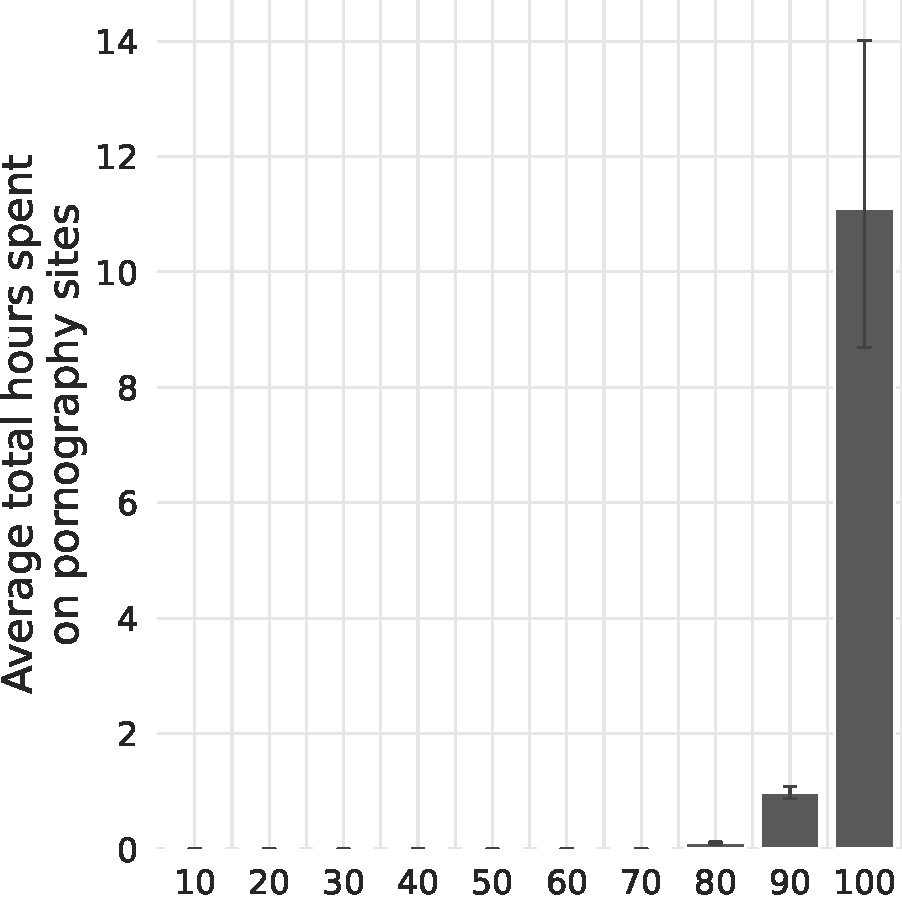
\includegraphics[width=\textwidth]{figs/mar/distribution_duration_on_adultsites_fullsample.pdf}
         \caption{Online pornography}
     \end{subfigure}
     \hfill
     \begin{subfigure}[b]{0.495\textwidth}
         \centering
         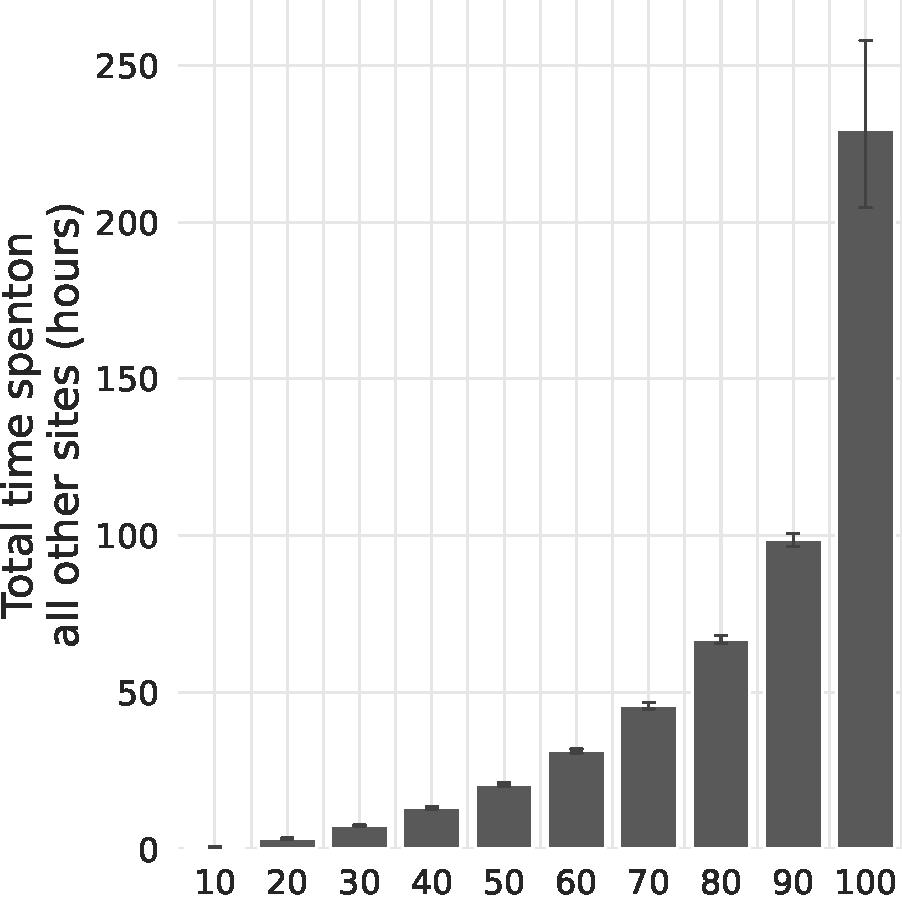
\includegraphics[width=\textwidth]{figs/mar/distribution_duration_on_nonadultsites_fullsample.pdf}
         \caption{Other online content}
     \end{subfigure}
\caption*{\footnotesize \emph{Notes:} 
    Each panel shows the total number of hours for the sample period.
    Individuals (n = 1135) are split into deciles, with each bin containing approximately the same number of individuals.
    The height of the bars indicates the mean of each bin. 
    Capped vertical bars are bootstrapped 95\% confidence intervals (n = 10,000).
    \cref{fig:distribution_duration_on_adultsites_fullsample} in main body.
    
}
\end{figure}


%========================================
% Quantile regressions
% Proportion of time spent on adult sites
%========================================
\begin{figure}[t]
	\centering
	\caption{Distribution of Partisan Differences in the Percentage of Time Spent on Pornographic Sites}
	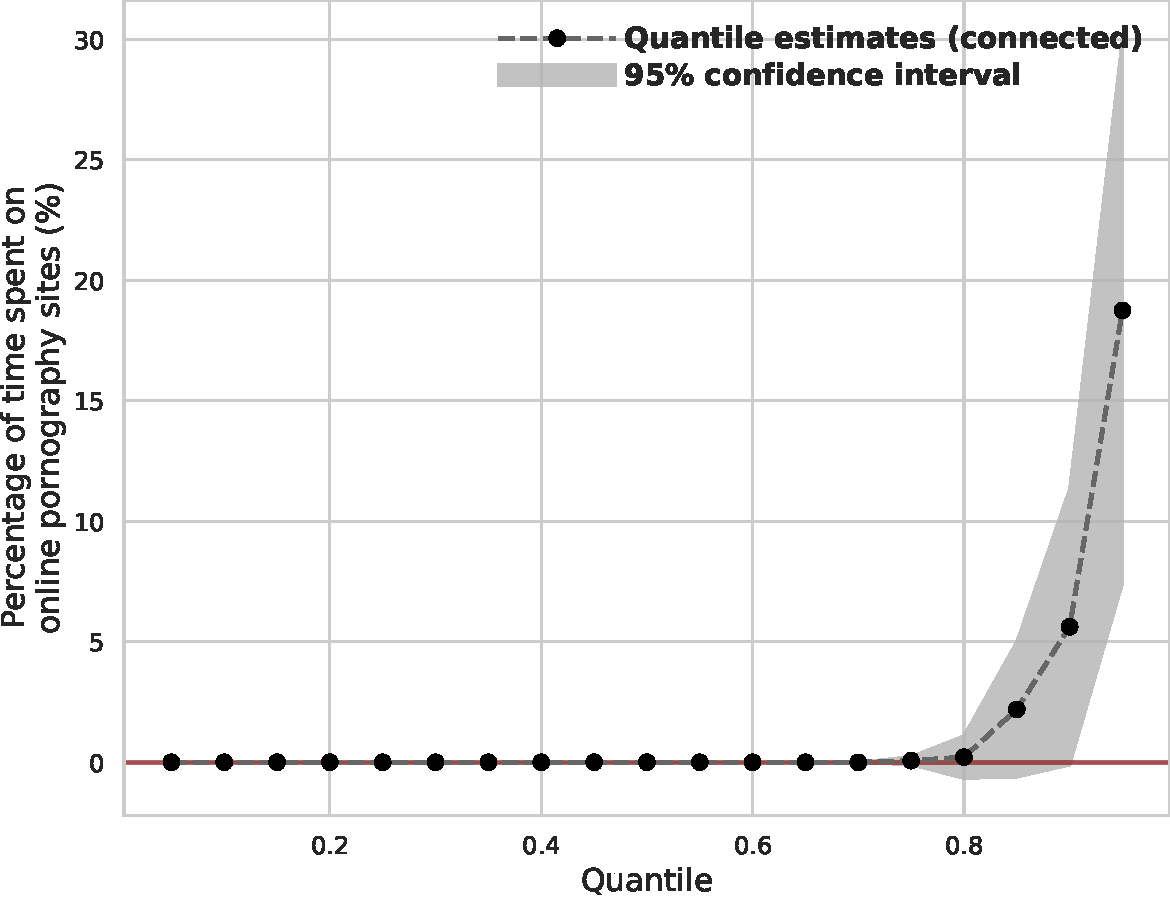
\includegraphics[width=.7\linewidth]{figs/mar/quantile_reg_proportion_duration_adult.pdf}
	\caption*{\footnotesize \emph{Notes:} 
		The dependent variable is the percentage of time individuals in our sample spent on pornographic sites.
		Each point indicates the difference between Republicans and Democrats and corresponds to a quantile regression at the quantile indicated by the x-axis.
		95\% confidence intervals constructed from standard errors.
		See \cref{fig:quantile_regression_prop_duration_covariates_mar} for the same plot controlling for individual characteristics.
            \cref{fig:quantile_regression_prop_duration} in main body.
	}
	\label{fig:quantile_regression_prop_duration_mar}
\end{figure}

%================================================================
% Fig of quantile regression estimates
% Percentage Time Spent on Adult Sites by Party (with covariates) 
%================================================================
\begin{figure}[!ht]
	\centering
	\caption{Quantile Estimates--Percentage of Time Spent on Pornographic Sites by Party (with covariates)}
	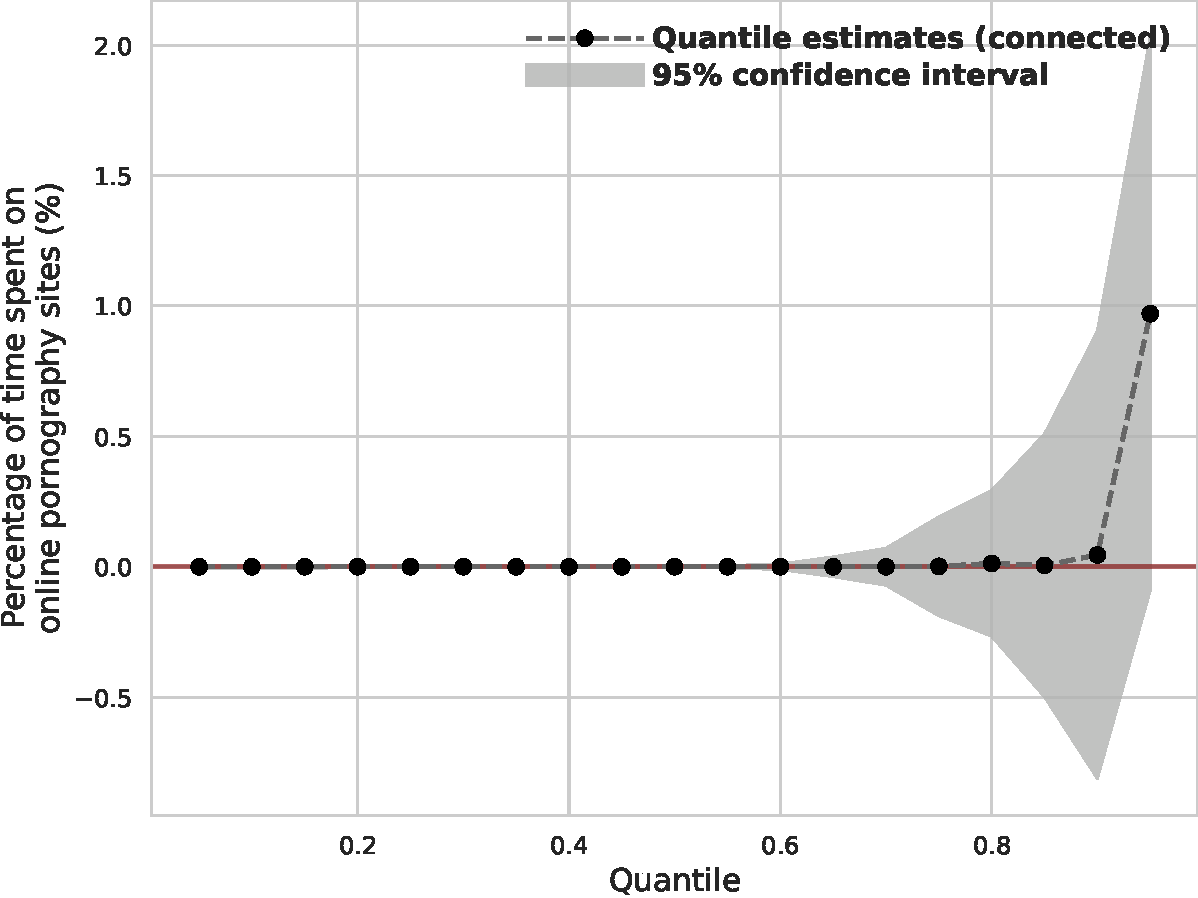
\includegraphics[width=.7\linewidth]{figs/mar/quantile_reg_covariates_proportion_duration_adult.pdf}
	\caption*{\footnotesize \emph{Notes:} 
		The dependent variable is the percentage of time individuals in our sample spent on pornographic sites.
		Each point indicates the difference between Republicans and Democrats and corresponds to a quantile regression at the quantile indicated by the x-axis.
		Covariates included on the right-hand side are: gender (Female/Male), race (White/Black/Hispanic/Asian/Others), education level (no HS/HS graduate/some college/college graduate), age and its quadratic, and region (NE/MW/S/W).
		95\% confidence intervals constructed from standard errors.
		See \cref{fig:quantile_regression_prop_duration_mar} for the same plot without covariates.
            \cref{fig:quantile_regression_prop_duration_covariates} in main body.
	}
	\label{fig:quantile_regression_prop_duration_covariates_mar}
\end{figure}



%=====================================================================
% Tabulated percentiles of the proportion of duration spent on adult sites
%=====================================================================
\begin{table}[ht] \centering \small \setlength\tabcolsep{10 pt}
	\caption{Percentage of Time Spent on Pornographic Sites (Conditional on having consumed pornography)}
	\label{tab:distribution_prop_duration_mar}
	\begin{adjustbox}{max width=\textwidth}
		\begin{tabular}{cr}
			\toprule
			\multicolumn{1}{c}{\textbf{Percentile}}&\multicolumn{1}{c}{\textbf{\% time}}\\
			\midrule
			0.00 &  0.0 \\
0.10 &  0.0 \\
0.20 &  0.2 \\
0.30 &  0.8 \\
0.40 &  1.5 \\
0.50 &  3.5 \\
0.60 &  5.8 \\
0.70 &  9.9 \\
0.80 & 17.1 \\
0.90 & 39.8 \\
0.95 & 61.2 \\
0.96 & 65.5 \\
0.97 & 70.7 \\
0.98 & 73.9 \\
0.99 & 81.9 \\
1.00 & 93.0 \\
			\bottomrule
		\end{tabular}
	\end{adjustbox}
	\caption*{\footnotesize \emph{Notes:} The table shows key percentiles (each of the ten deciles plus quantiles at the right tail) and their corresponding values for the percentage of time on pornography sites spent by individuals who consumed pornography in the sample period. The base number is the individual's own total time spent on the web. See \cref{tab:distribution_duration} for the distribution of total time spent on pornographic websites.
    See also \cref{tab:distribution_prop_duration}.
 }
\end{table}

%===============================================================================
% Tabulated splits by party and by percentiles for the proportion of time spent on adultsites
%===============================================================================
\begin{table}[ht] \centering \small \setlength\tabcolsep{10 pt}
	\caption{Percentage of Time Spent on Pornographic Sites by Party (Conditional on having consumed pornography)}
	\label{tab:distribution_prop_duration_party_mar}
	\begin{adjustbox}{max width=\textwidth}
		\begin{tabular}{crr}
			\toprule
			\multicolumn{1}{l}{\textbf{}}&\multicolumn{2}{c}{\textbf{\% time}}\\
			\cmidrule(l){2-3}
			\multicolumn{1}{l}{\textbf{Percentile}}&\multicolumn{1}{c}{\textbf{Republicans}}&\multicolumn{1}{c}{\textbf{Democrats}}\\
			\midrule
			0.00 &  0.0 &  0.0 \\
0.10 &  0.1 &  0.0 \\
0.20 &  0.5 &  0.1 \\
0.30 &  1.1 &  0.3 \\
0.40 &  2.5 &  1.0 \\
0.50 &  4.2 &  1.5 \\
0.60 &  7.8 &  3.8 \\
0.70 & 14.6 &  6.6 \\
0.80 & 25.1 & 13.4 \\
0.90 & 39.6 & 39.3 \\
0.95 & 52.8 & 57.3 
% 0.96 & 62.0 & 60.8 \\
% 0.97 & 65.7 & 66.5 \\
% 0.98 & 74.2 & 70.5 \\
% 0.99 & 85.6 & 74.6 \\
% 1.00 & 88.0 & 81.9 \\
			\bottomrule
		\end{tabular}
	\end{adjustbox}
	\caption*{\footnotesize \emph{Notes:} 
		The table shows splits by party and by key percentiles (each of the ten deciles plus quantiles at the right tail) for the percentage of time spent on pornography by individuals who consumed pornography in the sample period. 
        The base number is the individual's own total time spent on the web.
		See \cref{tab:distribution_duration_party} for the distribution in terms of percentage of time.
          See also \cref{tab:distribution_prop_duration_party}.
	}
\end{table}

\end{document}
